\documentclass[10pt]{article}

\usepackage{graphicx}
\usepackage{xcolor}
\usepackage{geometry}
\usepackage{amsmath}
\usepackage{amssymb}
\usepackage{amsthm}
\usepackage{booktabs}
\usepackage{array}
\usepackage{enumitem}
\usepackage{float}
\usepackage{placeins}
\usepackage[most]{tcolorbox}
\usepackage{caption}
\usepackage{xurl}
\captionsetup{font=small,labelfont=bf}
\captionsetup[figure]{name=Fig.}
\geometry{a4paper, top=2.4cm, bottom=2.6cm, left=2.6cm, right=2.6cm}
\setlist[itemize]{itemsep=0.25em, leftmargin=1.6em}


\usepackage[colorlinks=true, linkcolor=blue, citecolor=darkgray, urlcolor=blue,
  bookmarks=true, bookmarksnumbered=true, unicode=true]{hyperref}
\hypersetup{
  pdftitle={Real-time tunneling in light Lennard-Jones clusters: resource bounds, and why the classical-quantum window is not established},
  pdfauthor={Ammar Daskin},
  pdfkeywords={quantum simulation, tunneling, Lennard-Jones clusters, tensor networks, qubitization, resource bounds, negative result}}

\newcolumntype{L}[1]{>{\raggedright\arraybackslash}p{#1}}
\newcolumntype{C}[1]{>{\centering\arraybackslash}p{#1}}

% ---- numbers: every value that comes from a computation is a macro written by the data pipeline
\newcommand{\defnum}[2]{\expandafter\gdef\csname num@#1\endcsname{#2}}
\newcommand{\num}[1]{\ifcsname num@#1\endcsname\csname num@#1\endcsname\else{\bfseries\color{red}??#1}\fi}
\newcommand{\pending}[1]{{\color{red}\fbox{\footnotesize pending: #1}}}
% GENERATED by scripts/make_numbers.py -- do not edit.
\defnum{A}{8}%  config
\defnum{Asw}{200}%  config
\defnum{Bflop_txt}{\ensuremath{10^{20}}}%  config
\defnum{Bmem_txt}{\ensuremath{10^{12}}}%  config
\defnum{C_sel}{5019}%  quantum.npz
\defnum{Czero}{0.15}%  config
\defnum{ED_amp_N4}{\ensuremath{2.1\times10^{12}}}%  
\defnum{ED_grid}{4}%  larger_N.npz
\defnum{ED_grid_boson}{4}%  larger_N.npz
\defnum{ED_grid_last}{3}%  larger_N.npz
\defnum{ED_mem_N24}{\ensuremath{1\times10^{76}}}%  
\defnum{ED_mem_N4}{\ensuremath{3.3\times10^{14}}}%  
\defnum{ED_mode20}{8}%  larger_N.npz
\defnum{ED_mode20_boson}{17}%  larger_N.npz
\defnum{ED_ratio_N24}{\ensuremath{1\times10^{64}}}%  
\defnum{Ginf128}{210.5}%  mc_gamma_ledger.txt
\defnum{Ginf2D}{292.6}%  formula (Prop. 3) on the production grid
\defnum{Lx}{2.5}%  config
\defnum{Ly}{3.0}%  config
\defnum{MC_exp_N24}{\ensuremath{2.3\times10^{5}}}%  
\defnum{M_grid}{1200}%  config
\defnum{NQ}{88}%  quantum.npz
\defnum{Nhi_12}{88}%  quantum.npz
\defnum{Nhi_12_full}{88}%  quantum.npz
\defnum{Nhi_15}{53}%  quantum.npz
\defnum{Nhi_15_full}{37}%  quantum.npz
\defnum{Nhi_18}{19}%  quantum.npz
\defnum{Nhi_18_full}{11}%  quantum.npz
\defnum{Nmax_measured}{6}%  larger_N.npz
\defnum{Omax_N2}{1.00}%  uniform run N2_k12_int_c0.700_T200_dt1.npz
\defnum{Omax_N3}{1.00}%  uniform run N3_k12_int_c1.460_T200_dt1.npz
\defnum{Omax_N4}{1.00}%  uniform run N4_k12_int_c2.260_T200_dt1.npz
\defnum{Omax_N5}{1.00}%  uniform run N5_k12_int_c2.920_T200_dt1.npz
\defnum{Omax_N6}{0.99}%  uniform run N6_k12_int_c3.660_T200_dt1.npz
\defnum{Omin_N2}{0.10}%  uniform run N2_k12_int_c0.700_T200_dt1.npz
\defnum{Omin_N3}{0.15}%  uniform run N3_k12_int_c1.460_T200_dt1.npz
\defnum{Omin_N4}{0.25}%  uniform run N4_k12_int_c2.260_T200_dt1.npz
\defnum{Omin_N5}{0.27}%  uniform run N5_k12_int_c2.920_T200_dt1.npz
\defnum{Omin_N6}{0.37}%  uniform run N6_k12_int_c3.660_T200_dt1.npz
\defnum{Orev_N2}{1.00}%  uniform run N2_k12_int_c0.700_T200_dt1.npz (largest <O> after it first falls below 1/2)
\defnum{Orev_N3}{0.97}%  uniform run N3_k12_int_c1.460_T200_dt1.npz (largest <O> after it first falls below 1/2)
\defnum{Orev_N4}{0.81}%  uniform run N4_k12_int_c2.260_T200_dt1.npz (largest <O> after it first falls below 1/2)
\defnum{Orev_N5}{0.92}%  uniform run N5_k12_int_c2.920_T200_dt1.npz (largest <O> after it first falls below 1/2)
\defnum{Orev_N6}{0.90}%  uniform run N6_k12_int_c3.660_T200_dt1.npz (largest <O> after it first falls below 1/2)
\defnum{Qb_N10}{140}%  quantum.npz
\defnum{Qb_N16}{206}%  quantum.npz
\defnum{Qb_N24}{294}%  quantum.npz
\defnum{Qb_N4}{74}%  quantum.npz
\defnum{Qb_N40}{470}%  quantum.npz
\defnum{Qb_N8}{118}%  quantum.npz
\defnum{Qb_N88}{998}%  quantum.npz
\defnum{Qcap_txt}{1000}%  config
\defnum{S1_N2}{0.90}%  uniform run N2_k12_int_c0.700_T200_dt1.npz
\defnum{S1_N3}{1.32}%  uniform run N3_k12_int_c1.460_T200_dt1.npz
\defnum{S1_N4}{1.75}%  uniform run N4_k12_int_c2.260_T200_dt1.npz
\defnum{S1_N5}{1.88}%  uniform run N5_k12_int_c2.920_T200_dt1.npz
\defnum{S1_N5_k12}{1.88}%  ledger: k=12
\defnum{S1_N5_k16}{1.81}%  ledger: k=16
\defnum{S1_N5_k20}{1.80}%  ledger: k=20
\defnum{S1_N6}{1.93}%  uniform run N6_k12_int_c3.660_T200_dt1.npz
\defnum{S1_last}{1.93}%  larger_N.npz
\defnum{S24_opt}{12.1}%  larger_N.npz
\defnum{S24_pess}{22.2}%  larger_N.npz
\defnum{S24_sat}{13.3}%  larger_N.npz
\defnum{S2_N2}{0.53}%  ledger
\defnum{S2_N3}{0.88}%  ledger
\defnum{S2_N4}{1.67}%  ledger
\defnum{S2_N5}{1.85}%  ledger
\defnum{S2_N6}{2.05}%  ledger
\defnum{S2_cen}{0.90}%  uniform run N2_k12_int_c0.700_T200_dt1.npz
\defnum{S3_cen}{1.30}%  uniform run N3_k12_int_c1.460_T200_dt1.npz
\defnum{S4_cen}{2.33}%  uniform run N4_k12_int_c2.260_T200_dt1.npz
\defnum{S5_cen}{2.72}%  uniform run N5_k12_int_c2.920_T200_dt1.npz
\defnum{S6_cen}{3.26}%  uniform run N6_k12_int_c3.660_T200_dt1.npz
\defnum{S_N2_k12}{0.90}%  ledger
\defnum{S_N2_k16}{0.87}%  ledger
\defnum{S_N2_k20}{0.87}%  ledger
\defnum{S_N3_k12}{1.30}%  ledger
\defnum{S_N3_k16}{1.27}%  ledger
\defnum{S_N3_k20}{1.27}%  ledger
\defnum{S_N4_k12}{2.33}%  ledger
\defnum{S_N4_k16}{2.11}%  ledger
\defnum{S_N4_k20}{1.92}%  ledger
\defnum{S_N5_k12}{2.72}%  ledger
\defnum{S_N5_k16}{2.59}%  ledger
\defnum{S_N5_k20}{2.61}%  ledger
\defnum{S_N6_k12}{3.26}%  ledger
\defnum{Sbud_grid_N16}{8.0}%  
\defnum{Sbud_grid_N24}{7.8}%  
\defnum{Sbud_grid_N8}{8.4}%  
\defnum{Sbud_mode_N16}{13.8}%  
\defnum{Sbud_mode_N24}{13.5}%  
\defnum{Sbud_mode_N8}{14.3}%  
\defnum{Scen_corr_N4}{2.33}%  ledger: correlated start, k=12
\defnum{Scen_prod_N4}{4.81}%  ledger: product start, k=12
\defnum{Smax_N2}{0.90}%  uniform run N2_k12_int_c0.700_T200_dt1.npz
\defnum{Smax_N3}{1.37}%  uniform run N3_k12_int_c1.460_T200_dt1.npz
\defnum{Smax_N4}{2.54}%  uniform run N4_k12_int_c2.260_T200_dt1.npz
\defnum{Smax_N5}{2.93}%  uniform run N5_k12_int_c2.920_T200_dt1.npz
\defnum{Smax_N6}{3.70}%  uniform run N6_k12_int_c3.660_T200_dt1.npz
\defnum{Snat_N2}{0.90}%  uniform run N2_k12_int_c0.700_T200_dt1.npz
\defnum{Snat_N3}{1.30}%  uniform run N3_k12_int_c1.460_T200_dt1.npz
\defnum{Snat_N4}{2.33}%  uniform run N4_k12_int_c2.260_T200_dt1.npz
\defnum{Snat_N5}{2.72}%  uniform run N5_k12_int_c2.920_T200_dt1.npz
\defnum{Snat_N6}{3.26}%  uniform run N6_k12_int_c3.660_T200_dt1.npz
\defnum{Sperp_N2}{0.90}%  uniform run N2_k12_int_c0.700_T200_dt1.npz
\defnum{Sperp_N3}{1.29}%  uniform run N3_k12_int_c1.460_T200_dt1.npz
\defnum{Sperp_N4}{2.33}%  uniform run N4_k12_int_c2.260_T200_dt1.npz
\defnum{Sperp_N5}{2.62}%  uniform run N5_k12_int_c2.920_T200_dt1.npz
\defnum{Sperp_N6}{2.88}%  uniform run N6_k12_int_c3.660_T200_dt1.npz
\defnum{Szero}{5.33}%  quantum.npz
\defnum{TNflop_N24_opt}{\ensuremath{6.6\times10^{3}}}%  cost model / budget (grid)
\defnum{TNflop_N24_pess}{\ensuremath{9.9\times10^{12}}}%  cost model / budget (grid)
\defnum{TNflop_N24_sat}{\ensuremath{8.4\times10^{4}}}%  cost model / budget (grid)
\defnum{TNmem_N24_opt}{8.5}%  cost model / budget (grid)
\defnum{TNmem_N24_pess}{\ensuremath{1.1\times10^{7}}}%  cost model / budget (grid)
\defnum{TNmem_N24_sat}{46}%  cost model / budget (grid)
\defnum{T_N2}{200}%  ledger
\defnum{T_N3}{200}%  ledger
\defnum{T_N4}{200}%  ledger
\defnum{T_N5}{200}%  ledger
\defnum{T_N6}{200}%  ledger
\defnum{Tcap_txt}{\ensuremath{10^{12}}}%  config
\defnum{Tprot}{200}%  config [protocol]
\defnum{Tqub_N10}{\ensuremath{5.6\times10^{8}}}%  quantum.npz
\defnum{Tqub_N16}{\ensuremath{1.3\times10^{9}}}%  quantum.npz
\defnum{Tqub_N24}{\ensuremath{2.7\times10^{9}}}%  quantum.npz
\defnum{Tqub_N4}{\ensuremath{1.3\times10^{8}}}%  quantum.npz
\defnum{Tqub_N40}{\ensuremath{7.2\times10^{9}}}%  quantum.npz
\defnum{Tqub_N8}{\ensuremath{3.8\times10^{8}}}%  quantum.npz
\defnum{Tqub_N88}{\ensuremath{3.3\times10^{10}}}%  quantum.npz
\defnum{Ttrot_N10}{\ensuremath{3.2\times10^{13}}}%  quantum.npz
\defnum{Ttrot_N16}{\ensuremath{1.4\times10^{14}}}%  quantum.npz
\defnum{Ttrot_N24}{\ensuremath{4.9\times10^{14}}}%  quantum.npz
\defnum{Ttrot_N4}{\ensuremath{1.6\times10^{12}}}%  quantum.npz
\defnum{Ttrot_N40}{\ensuremath{2.3\times10^{15}}}%  quantum.npz
\defnum{Ttrot_N8}{\ensuremath{1.6\times10^{13}}}%  quantum.npz
\defnum{Ttrot_N88}{\ensuremath{2.5\times10^{16}}}%  quantum.npz
\defnum{Tw_hi}{200}%  config [studies]
\defnum{Tw_lo}{60}%  config [studies]
\defnum{Tw_mid}{120}%  config [studies]
\defnum{Vcap}{100}%  config
\defnum{Wg_N2}{0.90}%  uniform run N2_k12_int_c0.700_T200_dt1.npz
\defnum{Wg_N3}{1.42}%  uniform run N3_k12_int_c1.460_T200_dt1.npz
\defnum{Wg_N4}{2.44}%  uniform run N4_k12_int_c2.260_T200_dt1.npz
\defnum{Wg_N5}{2.88}%  uniform run N5_k12_int_c2.920_T200_dt1.npz
\defnum{Wg_N6}{3.72}%  uniform run N6_k12_int_c3.660_T200_dt1.npz
\defnum{Wpen}{30}%  config
\defnum{Wu_N2}{0.90}%  uniform run N2_k12_int_c0.700_T200_dt1.npz
\defnum{Wu_N3}{1.32}%  uniform run N3_k12_int_c1.460_T200_dt1.npz
\defnum{Wu_N4}{2.33}%  uniform run N4_k12_int_c2.260_T200_dt1.npz
\defnum{Wu_N5}{2.82}%  uniform run N5_k12_int_c2.920_T200_dt1.npz
\defnum{Wu_N6}{3.47}%  uniform run N6_k12_int_c3.660_T200_dt1.npz
\defnum{Wu_over_N5}{0.10}%  graph records
\defnum{Wu_over_N6}{0.21}%  graph records
\defnum{b_aux}{30}%  quantum.npz
\defnum{b_fix}{24}%  config
\defnum{bracket_N2}{0.00}%  uniform run N2_k12_int_c0.700_T200_dt1.npz
\defnum{bracket_N3}{0.08}%  uniform run N3_k12_int_c1.460_T200_dt1.npz
\defnum{bracket_N4}{0.21}%  uniform run N4_k12_int_c2.260_T200_dt1.npz
\defnum{bracket_N5}{0.31}%  uniform run N5_k12_int_c2.920_T200_dt1.npz
\defnum{bracket_N6}{0.82}%  uniform run N6_k12_int_c3.660_T200_dt1.npz
\defnum{c_prod}{0.45}%  fullgrid_resonance.npz / fullgrid_N2.npz
\defnum{c_res}{0.463}%  fullgrid_resonance.npz / fullgrid_N2.npz
\defnum{ch_A10_cap}{0.16}%  parameter_choice.npz <- data/studies/parameter_map/tier1_parameter_map.txt
\defnum{ch_A12_cap}{0.41}%  parameter_choice.npz <- data/studies/parameter_map/tier1_parameter_map.txt
\defnum{ch_A4_ov}{0.871}%  parameter_choice.npz <- data/studies/parameter_map/tier1_parameter_map.txt
\defnum{ch_A6_cap}{0.07}%  parameter_choice.npz <- data/studies/parameter_map/tier1_parameter_map.txt
\defnum{ch_A6_ov}{0.941}%  parameter_choice.npz <- data/studies/parameter_map/tier1_parameter_map.txt
\defnum{ch_A8_dE1}{0.1913}%  parameter_choice.npz <- data/studies/parameter_map/tier1_parameter_map.txt
\defnum{ch_A8_t1}{16.4}%  parameter_choice.npz <- data/studies/parameter_map/tier1_parameter_map.txt
\defnum{ch_A_deep}{8}%  parameter_choice.npz <- data/studies/parameter_map/tier1_parameter_map.txt
\defnum{ch_C0_05_cap}{0.19}%  parameter_choice.npz <- data/studies/parameter_map/tier1_parameter_map.txt
\defnum{ch_C0_05_ov}{0.88}%  parameter_choice.npz <- data/studies/parameter_map/tier1_parameter_map.txt
\defnum{ch_C0_0_cap}{0.26}%  parameter_choice.npz <- data/studies/parameter_map/tier1_parameter_map.txt
\defnum{ch_C0_0_ov}{0.74}%  parameter_choice.npz <- data/studies/parameter_map/tier1_parameter_map.txt
\defnum{ch_cap25_cap}{0.095}%  parameter_choice.npz <- data/studies/parameter_map/tier1_parameter_map.txt
\defnum{ch_cap_max}{0.1}%  parameter_choice.npz <- data/studies/parameter_map/tier1_parameter_map.txt
\defnum{ch_eps_c_hi}{0.41}%  parameter_choice.npz <- data/studies/parameter_map/tier1_parameter_map.txt
\defnum{ch_eps_c_lo}{0.39}%  parameter_choice.npz <- data/studies/parameter_map/tier1_parameter_map.txt
\defnum{ch_eps_dE_hi}{0.1904}%  parameter_choice.npz <- data/studies/parameter_map/tier1_parameter_map.txt
\defnum{ch_eps_dE_lo}{0.1901}%  parameter_choice.npz <- data/studies/parameter_map/tier1_parameter_map.txt
\defnum{ch_eps_n}{5}%  parameter_choice.npz <- data/studies/parameter_map/tier1_parameter_map.txt
\defnum{ch_eps_ov_hi}{0.979}%  parameter_choice.npz <- data/studies/parameter_map/tier1_parameter_map.txt
\defnum{ch_eps_ov_lo}{0.979}%  parameter_choice.npz <- data/studies/parameter_map/tier1_parameter_map.txt
\defnum{ch_eps_ov_rng}{0.979}%  parameter_choice.npz <- data/studies/parameter_map/tier1_parameter_map.txt
\defnum{ch_grid_gap}{1.3}%  parameter_choice.npz <- data/studies/parameter_map/tier1_parameter_map.txt
\defnum{ch_ov_min}{0.9}%  parameter_choice.npz <- data/studies/parameter_map/tier1_parameter_map.txt
\defnum{ch_prod_cap}{0.007}%  parameter_choice.npz <- data/studies/parameter_map/tier1_parameter_map.txt
\defnum{ch_prod_dE}{0.1901}%  parameter_choice.npz <- data/studies/parameter_map/tier1_parameter_map.txt
\defnum{ch_prod_ov}{0.979}%  parameter_choice.npz <- data/studies/parameter_map/tier1_parameter_map.txt
\defnum{ch_sig05_ov}{0.46}%  parameter_choice.npz <- data/studies/parameter_map/tier1_parameter_map.txt
\defnum{ch_t_A10}{25}%  parameter_choice.npz <- data/studies/parameter_map/tier1_parameter_map.txt
\defnum{ch_t_A12}{38}%  parameter_choice.npz <- data/studies/parameter_map/tier1_parameter_map.txt
\defnum{ch_t_A16}{81}%  parameter_choice.npz <- data/studies/parameter_map/tier1_parameter_map.txt
\defnum{chi2_N2}{4}%  ledger
\defnum{chi2_N3}{5}%  ledger
\defnum{chi2_N4}{19}%  ledger
\defnum{chi2_N5}{33}%  ledger
\defnum{chi2_N6}{113}%  ledger
\defnum{chi3_N2}{7}%  ledger
\defnum{chi3_N3}{10}%  ledger
\defnum{chi3_N4}{38}%  ledger
\defnum{chi3_N5}{74}%  ledger
\defnum{chi3_N5_k16}{105}%  uniform
\defnum{chi3_N5_k20}{118}%  uniform
\defnum{chi3_N6}{325}%  ledger
\defnum{chi6_N2}{11}%  ledger
\defnum{chi6_N3}{12}%  ledger
\defnum{chi6_N4}{118}%  ledger
\defnum{chi6_N5}{143}%  ledger
\defnum{chi6_N6}{1222}%  ledger
\defnum{chi_ratio_N5}{11.3}%  
\defnum{chi_shift}{5.1}%  larger_N.npz: log2 of chi(1e-3)/2^S at the largest simulated N
\defnum{chiratio_N2}{3.7}%  ledger
\defnum{chiratio_N3}{4.1}%  ledger
\defnum{chiratio_N4}{7.5}%  ledger
\defnum{chiratio_N5}{11.3}%  ledger
\defnum{chiratio_N6}{34.0}%  ledger
\defnum{chs_N3_A10_c}{1.48}%  parameter_scan_N*.npz (static scan: resonance found again for each A, k=12, correlated start)
\defnum{chs_N3_A10_dE}{0.125}%  parameter_scan_N*.npz (static scan: resonance found again for each A, k=12, correlated start)
\defnum{chs_N3_A10_ov}{0.96}%  parameter_scan_N*.npz (static scan: resonance found again for each A, k=12, correlated start)
\defnum{chs_N3_A12_c}{1.47}%  parameter_scan_N*.npz (static scan: resonance found again for each A, k=12, correlated start)
\defnum{chs_N3_A12_dE}{0.083}%  parameter_scan_N*.npz (static scan: resonance found again for each A, k=12, correlated start)
\defnum{chs_N3_A12_ov}{0.96}%  parameter_scan_N*.npz (static scan: resonance found again for each A, k=12, correlated start)
\defnum{chs_N3_A4_c}{1.24}%  parameter_scan_N*.npz (static scan: resonance found again for each A, k=12, correlated start)
\defnum{chs_N3_A4_dE}{0.314}%  parameter_scan_N*.npz (static scan: resonance found again for each A, k=12, correlated start)
\defnum{chs_N3_A4_ov}{0.82}%  parameter_scan_N*.npz (static scan: resonance found again for each A, k=12, correlated start)
\defnum{chs_N3_A6_c}{1.42}%  parameter_scan_N*.npz (static scan: resonance found again for each A, k=12, correlated start)
\defnum{chs_N3_A6_dE}{0.108}%  parameter_scan_N*.npz (static scan: resonance found again for each A, k=12, correlated start)
\defnum{chs_N3_A6_ov}{0.60}%  parameter_scan_N*.npz (static scan: resonance found again for each A, k=12, correlated start)
\defnum{chs_N3_A8_c}{1.47}%  parameter_scan_N*.npz (static scan: resonance found again for each A, k=12, correlated start)
\defnum{chs_N3_A8_dE}{0.191}%  parameter_scan_N*.npz (static scan: resonance found again for each A, k=12, correlated start)
\defnum{chs_N3_A8_ov}{0.93}%  parameter_scan_N*.npz (static scan: resonance found again for each A, k=12, correlated start)
\defnum{chs_N3_pass_list}{8, 10, 12}%  parameter_scan_N*.npz (static scan: resonance found again for each A, k=12, correlated start)
\defnum{chs_N3_pass_lo}{8}%  parameter_scan_N*.npz (static scan: resonance found again for each A, k=12, correlated start)
\defnum{chs_N4_A10_c}{2.26}%  parameter_scan_N*.npz (static scan: resonance found again for each A, k=12, correlated start)
\defnum{chs_N4_A10_dE}{0.105}%  parameter_scan_N*.npz (static scan: resonance found again for each A, k=12, correlated start)
\defnum{chs_N4_A10_ov}{0.81}%  parameter_scan_N*.npz (static scan: resonance found again for each A, k=12, correlated start)
\defnum{chs_N4_A12_c}{2.26}%  parameter_scan_N*.npz (static scan: resonance found again for each A, k=12, correlated start)
\defnum{chs_N4_A12_dE}{0.089}%  parameter_scan_N*.npz (static scan: resonance found again for each A, k=12, correlated start)
\defnum{chs_N4_A12_ov}{0.76}%  parameter_scan_N*.npz (static scan: resonance found again for each A, k=12, correlated start)
\defnum{chs_N4_A6_c}{2.22}%  parameter_scan_N*.npz (static scan: resonance found again for each A, k=12, correlated start)
\defnum{chs_N4_A6_dE}{0.092}%  parameter_scan_N*.npz (static scan: resonance found again for each A, k=12, correlated start)
\defnum{chs_N4_A6_ov}{0.38}%  parameter_scan_N*.npz (static scan: resonance found again for each A, k=12, correlated start)
\defnum{chs_N4_A8_c}{2.28}%  parameter_scan_N*.npz (static scan: resonance found again for each A, k=12, correlated start)
\defnum{chs_N4_A8_dE}{0.051}%  parameter_scan_N*.npz (static scan: resonance found again for each A, k=12, correlated start)
\defnum{chs_N4_A8_ov}{0.41}%  parameter_scan_N*.npz (static scan: resonance found again for each A, k=12, correlated start)
\defnum{chs_N4_pass_list}{none}%  parameter_scan_N*.npz (static scan: resonance found again for each A, k=12, correlated start)
\defnum{corr_N2}{0.90}%  ledger
\defnum{corr_N3}{1.30}%  ledger
\defnum{corr_N4}{2.33}%  ledger
\defnum{corr_N5}{2.72}%  ledger
\defnum{corr_N6}{3.26}%  ledger
\defnum{cr_N2_free_hi}{0.13}%  cosine_check.npz (residual of one cosine, as a fraction of the standard deviation of <O>(t))
\defnum{cr_N2_free_lo}{0.10}%  cosine_check.npz (residual of one cosine, as a fraction of the standard deviation of <O>(t))
\defnum{cr_N2_hi}{0.14}%  cosine_check.npz (residual of one cosine, as a fraction of the standard deviation of <O>(t))
\defnum{cr_N2_lo}{0.10}%  cosine_check.npz (residual of one cosine, as a fraction of the standard deviation of <O>(t))
\defnum{cr_N3_free_hi}{0.15}%  cosine_check.npz (residual of one cosine, as a fraction of the standard deviation of <O>(t))
\defnum{cr_N3_free_lo}{0.12}%  cosine_check.npz (residual of one cosine, as a fraction of the standard deviation of <O>(t))
\defnum{cr_N3_hi}{0.15}%  cosine_check.npz (residual of one cosine, as a fraction of the standard deviation of <O>(t))
\defnum{cr_N3_lo}{0.12}%  cosine_check.npz (residual of one cosine, as a fraction of the standard deviation of <O>(t))
\defnum{cr_N3_nk}{6}%  cosine_check.npz (residual of one cosine, as a fraction of the standard deviation of <O>(t))
\defnum{cr_N4_k12_fix}{1.00}%  cosine_check.npz (residual of one cosine, as a fraction of the standard deviation of <O>(t))
\defnum{cr_N4_k12_free}{0.72}%  cosine_check.npz (residual of one cosine, as a fraction of the standard deviation of <O>(t))
\defnum{cr_N4_k16_fix}{1.00}%  cosine_check.npz (residual of one cosine, as a fraction of the standard deviation of <O>(t))
\defnum{cr_N4_k16_free}{0.41}%  cosine_check.npz (residual of one cosine, as a fraction of the standard deviation of <O>(t))
\defnum{cr_N4_k20_fix}{0.18}%  cosine_check.npz (residual of one cosine, as a fraction of the standard deviation of <O>(t))
\defnum{cr_N4_k20_free}{0.17}%  cosine_check.npz (residual of one cosine, as a fraction of the standard deviation of <O>(t))
\defnum{cr_N5_k12_fix}{0.85}%  cosine_check.npz (residual of one cosine, as a fraction of the standard deviation of <O>(t))
\defnum{cr_N5_k12_free}{0.74}%  cosine_check.npz (residual of one cosine, as a fraction of the standard deviation of <O>(t))
\defnum{cr_N5_k16_fix}{1.00}%  cosine_check.npz (residual of one cosine, as a fraction of the standard deviation of <O>(t))
\defnum{cr_N5_k16_free}{0.48}%  cosine_check.npz (residual of one cosine, as a fraction of the standard deviation of <O>(t))
\defnum{cr_N5_k20_fix}{1.00}%  cosine_check.npz (residual of one cosine, as a fraction of the standard deviation of <O>(t))
\defnum{cr_N5_k20_free}{0.24}%  cosine_check.npz (residual of one cosine, as a fraction of the standard deviation of <O>(t))
\defnum{cr_N5_k20_wratio}{2.2}%  cosine_check.npz (residual of one cosine, as a fraction of the standard deviation of <O>(t))
\defnum{cr_N6_k12_fix}{0.99}%  cosine_check.npz (residual of one cosine, as a fraction of the standard deviation of <O>(t))
\defnum{cr_N6_k12_free}{0.55}%  cosine_check.npz (residual of one cosine, as a fraction of the standard deviation of <O>(t))
\defnum{cr_N6_k12_wratio}{2.5}%  cosine_check.npz (residual of one cosine, as a fraction of the standard deviation of <O>(t))
\defnum{cstar_N2}{0.70}%  uniform run N2_k12_int_c0.700_T200_dt1.npz
\defnum{cstar_N2_k12}{0.70}%  ledger
\defnum{cstar_N2_k16}{0.70}%  ledger
\defnum{cstar_N2_k20}{0.70}%  ledger
\defnum{cstar_N3}{1.46}%  uniform run N3_k12_int_c1.460_T200_dt1.npz
\defnum{cstar_N3_k12}{1.46}%  ledger
\defnum{cstar_N3_k16}{1.36}%  ledger
\defnum{cstar_N3_k20}{1.31}%  ledger
\defnum{cstar_N4}{2.26}%  uniform run N4_k12_int_c2.260_T200_dt1.npz
\defnum{cstar_N4_k12}{2.26}%  ledger
\defnum{cstar_N4_k16}{2.14}%  ledger
\defnum{cstar_N4_k20}{2.02}%  ledger
\defnum{cstar_N5}{2.92}%  uniform run N5_k12_int_c2.920_T200_dt1.npz
\defnum{cstar_N5_k12}{2.92}%  ledger
\defnum{cstar_N5_k16}{2.72}%  ledger
\defnum{cstar_N5_k20}{2.62}%  ledger
\defnum{cstar_N6}{3.66}%  uniform run N6_k12_int_c3.660_T200_dt1.npz
\defnum{cstar_N6_k12}{3.66}%  ledger
\defnum{d23}{0.39}%  graph records
\defnum{d34}{1.04}%  graph records
\defnum{d45}{0.38}%  graph records
\defnum{d45_note}{}%  empty: every N is a uniform run
\defnum{d56}{0.54}%  graph records
\defnum{dE2grid}{0.190}%  quantum.npz
\defnum{dE_N2}{0.180}%  ledger
\defnum{dE_N2_k12}{0.180}%  ledger
\defnum{dE_N2_k16}{0.185}%  ledger
\defnum{dE_N2_k20}{0.192}%  ledger
\defnum{dE_N3}{0.189}%  ledger
\defnum{dE_N3_k12}{0.189}%  ledger
\defnum{dE_N3_k16}{0.191}%  ledger
\defnum{dE_N3_k20}{0.193}%  ledger
\defnum{dE_N4}{0.052}%  ledger
\defnum{dE_N4_k12}{0.052}%  ledger
\defnum{dE_N4_k16}{0.104}%  ledger
\defnum{dE_N4_k20}{0.218}%  ledger
\defnum{dE_N5}{0.152}%  ledger
\defnum{dE_N5_k12}{0.152}%  ledger
\defnum{dE_N5_k16}{0.107}%  ledger
\defnum{dE_N5_k20}{0.105}%  ledger
\defnum{dE_N6}{0.173}%  ledger
\defnum{dE_N6_k12}{0.173}%  ledger
\defnum{dE_prod}{0.1896}%  fullgrid_resonance.npz / fullgrid_N2.npz
\defnum{dE_res}{0.1919}%  fullgrid_resonance.npz / fullgrid_N2.npz
\defnum{dS1_23}{0.41}%  graph records
\defnum{dS1_34}{0.43}%  graph records
\defnum{dS1_45}{0.14}%  graph records
\defnum{dS1_56}{0.05}%  graph records
\defnum{dS1k16_23}{0.40}%  ledger: k=16
\defnum{dS1k16_34}{0.40}%  ledger: k=16
\defnum{dS1k16_45}{0.14}%  ledger: k=16
\defnum{dS1k20_23}{0.39}%  ledger: k=20
\defnum{dS1k20_34}{0.30}%  ledger: k=20
\defnum{dS1k20_45}{0.24}%  ledger: k=20
\defnum{dScen_45_k12}{0.38}%  ledger: k=12
\defnum{dScen_45_k16}{0.48}%  ledger: k=16
\defnum{dScen_45_k20}{0.69}%  ledger: k=20
\defnum{d_grid}{1200}%  config
\defnum{d_mode}{20}%  config
\defnum{dag_N2}{}%  dagger if the point is from the earlier protocol
\defnum{dag_N3}{}%  dagger if the point is from the earlier protocol
\defnum{dag_N4}{}%  dagger if the point is from the earlier protocol
\defnum{dag_N5}{}%  dagger if the point is from the earlier protocol
\defnum{dag_N6}{}%  dagger if the point is from the earlier protocol
\defnum{dag_off}{}%  dagger if from the earlier protocol
\defnum{dbl_N2}{yes}%  ledger
\defnum{dbl_N2_k12}{yes}%  ledger
\defnum{dbl_N2_k16}{yes}%  ledger
\defnum{dbl_N2_k20}{yes}%  ledger
\defnum{dbl_N3}{yes}%  ledger
\defnum{dbl_N3_k12}{yes}%  ledger
\defnum{dbl_N3_k16}{yes}%  ledger
\defnum{dbl_N3_k20}{yes}%  ledger
\defnum{dbl_N4}{no}%  ledger
\defnum{dbl_N4_k12}{no}%  ledger
\defnum{dbl_N4_k16}{no}%  ledger
\defnum{dbl_N4_k20}{yes}%  ledger
\defnum{dbl_N5}{no}%  ledger
\defnum{dbl_N5_k12}{no}%  ledger
\defnum{dbl_N5_k16}{no}%  ledger
\defnum{dbl_N5_k20}{no}%  ledger
\defnum{dbl_N6}{no}%  ledger
\defnum{dbl_N6_k12}{no}%  ledger
\defnum{devmax_N2}{0.00}%  uniform run N2_k12_int_c0.700_T200_dt1.npz
\defnum{devmax_N3}{-0.12}%  uniform run N3_k12_int_c1.460_T200_dt1.npz
\defnum{devmax_N4}{0.00}%  uniform run N4_k12_int_c2.260_T200_dt1.npz
\defnum{devmax_N5}{0.02}%  uniform run N5_k12_int_c2.920_T200_dt1.npz
\defnum{devmax_N6}{0.00}%  uniform run N6_k12_int_c3.660_T200_dt1.npz
\defnum{devmin_N2}{0.00}%  uniform run N2_k12_int_c0.700_T200_dt1.npz
\defnum{devmin_N3}{-0.22}%  uniform run N3_k12_int_c1.460_T200_dt1.npz
\defnum{devmin_N4}{-0.22}%  uniform run N4_k12_int_c2.260_T200_dt1.npz
\defnum{devmin_N5}{-0.30}%  uniform run N5_k12_int_c2.920_T200_dt1.npz
\defnum{devmin_N6}{-0.48}%  uniform run N6_k12_int_c3.660_T200_dt1.npz
\defnum{dtsnap}{1.0}%  config [protocol]
\defnum{dx}{0.125}%  config
\defnum{dy}{0.200}%  config
\defnum{edge_N10}{19.9}%  quantum.npz
\defnum{edge_N10_full}{18.4}%  quantum.npz
\defnum{edge_N16}{18.6}%  quantum.npz
\defnum{edge_N16_full}{17.3}%  quantum.npz
\defnum{edge_N24}{17.4}%  quantum.npz
\defnum{edge_N24_full}{16.2}%  quantum.npz
\defnum{edge_N4}{22.2}%  quantum.npz
\defnum{edge_N40}{15.9}%  quantum.npz
\defnum{edge_N40_full}{14.8}%  quantum.npz
\defnum{edge_N4_full}{20.5}%  quantum.npz
\defnum{edge_N8}{20.5}%  quantum.npz
\defnum{edge_N88}{13.5}%  quantum.npz
\defnum{edge_N88_full}{12.7}%  quantum.npz
\defnum{edge_N8_full}{19.0}%  quantum.npz
\defnum{edge_drop_8_88}{7.0}%  quantum.npz
\defnum{edge_shift_8}{1.5}%  quantum.npz
\defnum{edge_trot_N10}{1.6}%  quantum.npz
\defnum{edge_trot_N16}{none}%  quantum.npz
\defnum{edge_trot_N24}{none}%  quantum.npz
\defnum{edge_trot_N4}{7.2}%  quantum.npz
\defnum{edge_trot_N40}{none}%  quantum.npz
\defnum{edge_trot_N8}{3.2}%  quantum.npz
\defnum{edge_trot_N88}{none}%  quantum.npz
\defnum{eps_LJ}{2}%  config
\defnum{eps_prec}{\ensuremath{10^{-3}}}%  config
\defnum{fit_Sinf}{2.12}%  
\defnum{fit_npts}{4}%  larger_N.npz: points N=3.. fitted (the curve is anchored at N=2)
\defnum{fit_tau}{2.0}%  
\defnum{fu_B2_N2_k12}{0.976}%  data/followup/stage1/N*_k*_c*.npz
\defnum{fu_B2_N2_k16}{0.976}%  data/followup/stage1/N*_k*_c*.npz
\defnum{fu_B2_N2_k20}{0.978}%  data/followup/stage1/N*_k*_c*.npz
\defnum{fu_B2_N3_k12}{0.938}%  data/followup/stage1/N*_k*_c*.npz
\defnum{fu_B2_N3_k16}{0.952}%  data/followup/stage1/N*_k*_c*.npz
\defnum{fu_B2_N3_k20}{0.955}%  data/followup/stage1/N*_k*_c*.npz
\defnum{fu_B2_N4_k12}{0.668}%  data/followup/stage1/N*_k*_c*.npz
\defnum{fu_B2_N4_k16}{0.845}%  data/followup/stage1/N*_k*_c*.npz
\defnum{fu_B2_N4_k20}{0.906}%  data/followup/stage1/N*_k*_c*.npz
\defnum{fu_B2_N4_k24}{0.921}%  data/followup/stage1/N*_k*_c*.npz
\defnum{fu_B2_N4_k28}{0.931}%  data/followup/stage1/N*_k*_c*.npz
\defnum{fu_B2_N4_k32}{0.934}%  data/followup/stage1/N*_k*_c*.npz
\defnum{fu_B2_N4_kmax}{0.934}%  data/followup/stage1/N*_k*_c*.npz
\defnum{fu_B2_N5_k12}{0.683}%  data/followup/stage1/N*_k*_c*.npz
\defnum{fu_B2_N5_k16}{0.780}%  data/followup/stage1/N*_k*_c*.npz
\defnum{fu_B2_N5_k20}{0.812}%  data/followup/stage1/N*_k*_c*.npz
\defnum{fu_B2_N5_k24}{0.836}%  data/followup/stage1/N*_k*_c*.npz
\defnum{fu_B2_N6_k12}{0.729}%  data/followup/stage1/N*_k*_c*.npz
\defnum{fu_Emax_N3_k12}{3.34}%  data/followup/static_checks/levels_N*_k*_c*.npz
\defnum{fu_Emax_N3_k16}{3.40}%  data/followup/static_checks/levels_N*_k*_c*.npz
\defnum{fu_Emax_N4_k12}{2.14}%  data/followup/static_checks/levels_N*_k*_c*.npz
\defnum{fu_J_N2_k12}{0.090}%  data/followup/stage1/N*_k*_c*.npz
\defnum{fu_J_N2_k16}{0.092}%  data/followup/stage1/N*_k*_c*.npz
\defnum{fu_J_N2_k20}{0.096}%  data/followup/stage1/N*_k*_c*.npz
\defnum{fu_J_N3_k12}{0.094}%  data/followup/stage1/N*_k*_c*.npz
\defnum{fu_J_N3_k16}{0.095}%  data/followup/stage1/N*_k*_c*.npz
\defnum{fu_J_N3_k20}{0.097}%  data/followup/stage1/N*_k*_c*.npz
\defnum{fu_J_N4_k12}{0.092}%  data/followup/stage1/N*_k*_c*.npz
\defnum{fu_J_N4_k16}{0.113}%  data/followup/stage1/N*_k*_c*.npz
\defnum{fu_J_N4_k20}{0.109}%  data/followup/stage1/N*_k*_c*.npz
\defnum{fu_J_N4_k24}{0.110}%  data/followup/stage1/N*_k*_c*.npz
\defnum{fu_J_N4_k28}{0.110}%  data/followup/stage1/N*_k*_c*.npz
\defnum{fu_J_N4_k32}{0.111}%  data/followup/stage1/N*_k*_c*.npz
\defnum{fu_J_N5_k12}{0.181}%  data/followup/stage1/N*_k*_c*.npz
\defnum{fu_J_N5_k16}{0.114}%  data/followup/stage1/N*_k*_c*.npz
\defnum{fu_J_N5_k20}{0.117}%  data/followup/stage1/N*_k*_c*.npz
\defnum{fu_J_N5_k24}{0.126}%  data/followup/stage1/N*_k*_c*.npz
\defnum{fu_J_N6_k12}{0.218}%  data/followup/stage1/N*_k*_c*.npz
\defnum{fu_Jlv_N3_k12}{0.094}%  data/followup/static_checks/levels_N*_k*_c*.npz
\defnum{fu_Jlv_N3_k16}{0.095}%  data/followup/static_checks/levels_N*_k*_c*.npz
\defnum{fu_Jlv_N4_k12}{0.092}%  data/followup/static_checks/levels_N*_k*_c*.npz
\defnum{fu_Kx}{316}%  pi^2 / (2 dx^2), dx from config.toml
\defnum{fu_N4_Jhi}{0.111}%  data/followup/stage1/N*_k*_c*.npz
\defnum{fu_N4_Jlo}{0.109}%  data/followup/stage1/N*_k*_c*.npz
\defnum{fu_N4_dB2_32_12}{0.267}%  data/followup/stage1/N*_k*_c*.npz
\defnum{fu_N4_dB2_32_20}{0.029}%  data/followup/stage1/N*_k*_c*.npz
\defnum{fu_N5_cov_k24}{0.92}%  data/followup/stage1/N*_k*_c*.npz
\defnum{fu_N5_dB2_24_20}{0.023}%  data/followup/stage1/N*_k*_c*.npz
\defnum{fu_N5_dress_over_N4_k20}{2.0}%  data/followup/stage1/N*_k*_c*.npz
\defnum{fu_Ntop_hi}{11}%  max over the two lines
\defnum{fu_Ntop_k12}{10}%  line through c*(N) reaching fu_ctop
\defnum{fu_Ntop_k20}{11}%  line through c*(N) reaching fu_ctop
\defnum{fu_Ntop_lo}{10}%  min over the two lines
\defnum{fu_Rstart_N3_k12}{0.9999}%  data/followup/static_checks/levels_N*_k*_c*.npz
\defnum{fu_Rstart_N3_k16}{0.9999}%  data/followup/static_checks/levels_N*_k*_c*.npz
\defnum{fu_Rstart_N4_k12}{0.9997}%  data/followup/static_checks/levels_N*_k*_c*.npz
\defnum{fu_band_gap_N3}{1.05}%  same: gap above the band
\defnum{fu_band_gap_N4}{1.04}%  same: gap above the band
\defnum{fu_band_n_N3}{12}%  data/followup/stage1/untilted_*_C00.npz (level before the largest gap in the lowest 60)
\defnum{fu_band_n_N4}{24}%  data/followup/stage1/untilted_*_C00.npz (level before the largest gap in the lowest 60)
\defnum{fu_band_w_N3}{0.41}%  same: width of the band
\defnum{fu_band_w_N4}{0.29}%  same: width of the band
\defnum{fu_cos_M05_N2}{3}%  data/followup/freq_signal_analysis.log
\defnum{fu_cos_M05_N3}{3}%  data/followup/freq_signal_analysis.log
\defnum{fu_cos_M05_N4}{5}%  data/followup/freq_signal_analysis.log
\defnum{fu_cos_M05_N5}{8}%  data/followup/freq_signal_analysis.log
\defnum{fu_cos_M05_N6}{\ensuremath{>}8}%  data/followup/freq_signal_analysis.log
\defnum{fu_cos_M10_N2}{1}%  data/followup/freq_signal_analysis.log
\defnum{fu_cos_M10_N3}{2}%  data/followup/freq_signal_analysis.log
\defnum{fu_cos_M10_N4}{3}%  data/followup/freq_signal_analysis.log
\defnum{fu_cos_M10_N5}{4}%  data/followup/freq_signal_analysis.log
\defnum{fu_cos_M10_N6}{\ensuremath{>}8}%  data/followup/freq_signal_analysis.log
\defnum{fu_cos_k_N2}{20}%  data/followup/freq_signal_analysis.log
\defnum{fu_cos_k_N3}{32}%  data/followup/freq_signal_analysis.log
\defnum{fu_cos_k_N4}{20}%  data/followup/freq_signal_analysis.log
\defnum{fu_cos_k_N5}{20}%  data/followup/freq_signal_analysis.log
\defnum{fu_cos_k_N6}{12}%  data/followup/freq_signal_analysis.log
\defnum{fu_cos_r3_N2}{0.02}%  data/followup/freq_signal_analysis.log
\defnum{fu_cos_r3_N3}{0.04}%  data/followup/freq_signal_analysis.log
\defnum{fu_cos_r3_N4}{0.06}%  data/followup/freq_signal_analysis.log
\defnum{fu_cos_r3_N5}{0.12}%  data/followup/freq_signal_analysis.log
\defnum{fu_cos_r3_N6}{0.20}%  data/followup/freq_signal_analysis.log
\defnum{fu_cov_N2_k12}{1.000}%  data/followup/stage1/N*_k*_c*.npz
\defnum{fu_cov_N2_k16}{1.000}%  data/followup/stage1/N*_k*_c*.npz
\defnum{fu_cov_N2_k20}{1.000}%  data/followup/stage1/N*_k*_c*.npz
\defnum{fu_cov_N3_k12}{1.000}%  data/followup/stage1/N*_k*_c*.npz
\defnum{fu_cov_N3_k16}{1.000}%  data/followup/stage1/N*_k*_c*.npz
\defnum{fu_cov_N3_k20}{1.000}%  data/followup/stage1/N*_k*_c*.npz
\defnum{fu_cov_N4_k12}{0.993}%  data/followup/stage1/N*_k*_c*.npz
\defnum{fu_cov_N4_k16}{0.985}%  data/followup/stage1/N*_k*_c*.npz
\defnum{fu_cov_N4_k20}{0.986}%  data/followup/stage1/N*_k*_c*.npz
\defnum{fu_cov_N4_k24}{0.975}%  data/followup/stage1/N*_k*_c*.npz
\defnum{fu_cov_N4_k28}{0.977}%  data/followup/stage1/N*_k*_c*.npz
\defnum{fu_cov_N4_k32}{0.976}%  data/followup/stage1/N*_k*_c*.npz
\defnum{fu_cov_N5_k12}{0.971}%  data/followup/stage1/N*_k*_c*.npz
\defnum{fu_cov_N5_k16}{0.942}%  data/followup/stage1/N*_k*_c*.npz
\defnum{fu_cov_N5_k20}{0.943}%  data/followup/stage1/N*_k*_c*.npz
\defnum{fu_cov_N5_k24}{0.918}%  data/followup/stage1/N*_k*_c*.npz
\defnum{fu_cov_N6_k12}{0.936}%  data/followup/stage1/N*_k*_c*.npz
\defnum{fu_cs_N2_k12}{0.70}%  data/followup/stage1/N*_k*_c*.npz (tilt of the file name)
\defnum{fu_cs_N2_k16}{0.70}%  data/followup/stage1/N*_k*_c*.npz (tilt of the file name)
\defnum{fu_cs_N2_k20}{0.70}%  data/followup/stage1/N*_k*_c*.npz (tilt of the file name)
\defnum{fu_cs_N3_k12}{1.46}%  data/followup/stage1/N*_k*_c*.npz (tilt of the file name)
\defnum{fu_cs_N3_k16}{1.36}%  data/followup/stage1/N*_k*_c*.npz (tilt of the file name)
\defnum{fu_cs_N3_k20}{1.31}%  data/followup/stage1/N*_k*_c*.npz (tilt of the file name)
\defnum{fu_cs_N4_k12}{2.26}%  data/followup/stage1/N*_k*_c*.npz (tilt of the file name)
\defnum{fu_cs_N4_k16}{2.14}%  data/followup/stage1/N*_k*_c*.npz (tilt of the file name)
\defnum{fu_cs_N4_k20}{2.02}%  data/followup/stage1/N*_k*_c*.npz (tilt of the file name)
\defnum{fu_cs_N4_k24}{1.94}%  data/followup/stage1/N*_k*_c*.npz (tilt of the file name)
\defnum{fu_cs_N4_k28}{1.87}%  data/followup/stage1/N*_k*_c*.npz (tilt of the file name)
\defnum{fu_cs_N4_k32}{1.82}%  data/followup/stage1/N*_k*_c*.npz (tilt of the file name)
\defnum{fu_cs_N5_k12}{2.92}%  data/followup/stage1/N*_k*_c*.npz (tilt of the file name)
\defnum{fu_cs_N5_k16}{2.72}%  data/followup/stage1/N*_k*_c*.npz (tilt of the file name)
\defnum{fu_cs_N5_k20}{2.62}%  data/followup/stage1/N*_k*_c*.npz (tilt of the file name)
\defnum{fu_cs_N5_k24}{2.57}%  data/followup/stage1/N*_k*_c*.npz (tilt of the file name)
\defnum{fu_cs_N6_k12}{3.66}%  data/followup/stage1/N*_k*_c*.npz (tilt of the file name)
\defnum{fu_cslope_k12}{0.74}%  data/followup/stage1/N*_k*_c*.npz (least-squares line through c*(N))
\defnum{fu_cslope_k20}{0.65}%  data/followup/stage1/N*_k*_c*.npz (least-squares line through c*(N))
\defnum{fu_cstep_hi_k12}{0.80}%  data/followup/stage1/N*_k*_c*.npz
\defnum{fu_cstep_hi_k20}{0.71}%  data/followup/stage1/N*_k*_c*.npz
\defnum{fu_cstep_lo_k12}{0.66}%  data/followup/stage1/N*_k*_c*.npz
\defnum{fu_cstep_lo_k20}{0.60}%  data/followup/stage1/N*_k*_c*.npz
\defnum{fu_ctop}{6.4}%  followup_data.c_top (one-particle tilted well, finite differences)
\defnum{fu_dress_N2_k12}{0.024}%  data/followup/stage1/N*_k*_c*.npz
\defnum{fu_dress_N2_k16}{0.024}%  data/followup/stage1/N*_k*_c*.npz
\defnum{fu_dress_N2_k20}{0.022}%  data/followup/stage1/N*_k*_c*.npz
\defnum{fu_dress_N3_k12}{0.062}%  data/followup/stage1/N*_k*_c*.npz
\defnum{fu_dress_N3_k16}{0.048}%  data/followup/stage1/N*_k*_c*.npz
\defnum{fu_dress_N3_k20}{0.045}%  data/followup/stage1/N*_k*_c*.npz
\defnum{fu_dress_N4_k12}{0.332}%  data/followup/stage1/N*_k*_c*.npz
\defnum{fu_dress_N4_k16}{0.155}%  data/followup/stage1/N*_k*_c*.npz
\defnum{fu_dress_N4_k20}{0.094}%  data/followup/stage1/N*_k*_c*.npz
\defnum{fu_dress_N4_k24}{0.079}%  data/followup/stage1/N*_k*_c*.npz
\defnum{fu_dress_N4_k28}{0.069}%  data/followup/stage1/N*_k*_c*.npz
\defnum{fu_dress_N4_k32}{0.066}%  data/followup/stage1/N*_k*_c*.npz
\defnum{fu_dress_N4_kmax}{0.066}%  data/followup/stage1/N*_k*_c*.npz
\defnum{fu_dress_N5_k12}{0.317}%  data/followup/stage1/N*_k*_c*.npz
\defnum{fu_dress_N5_k16}{0.220}%  data/followup/stage1/N*_k*_c*.npz
\defnum{fu_dress_N5_k20}{0.188}%  data/followup/stage1/N*_k*_c*.npz
\defnum{fu_dress_N5_k24}{0.164}%  data/followup/stage1/N*_k*_c*.npz
\defnum{fu_dress_N6_k12}{0.271}%  data/followup/stage1/N*_k*_c*.npz
\defnum{fu_far_N2_k12}{0.010}%  data/followup/stage1/N*_k*_c*.npz
\defnum{fu_far_N2_k16}{0.012}%  data/followup/stage1/N*_k*_c*.npz
\defnum{fu_far_N2_k20}{0.013}%  data/followup/stage1/N*_k*_c*.npz
\defnum{fu_far_N3_k12}{0.017}%  data/followup/stage1/N*_k*_c*.npz
\defnum{fu_far_N3_k16}{0.030}%  data/followup/stage1/N*_k*_c*.npz
\defnum{fu_far_N3_k20}{0.028}%  data/followup/stage1/N*_k*_c*.npz
\defnum{fu_far_N4_k12}{0.027}%  data/followup/stage1/N*_k*_c*.npz
\defnum{fu_far_N4_k16}{0.026}%  data/followup/stage1/N*_k*_c*.npz
\defnum{fu_far_N4_k20}{0.024}%  data/followup/stage1/N*_k*_c*.npz
\defnum{fu_far_N4_k24}{0.012}%  data/followup/stage1/N*_k*_c*.npz
\defnum{fu_far_N4_k28}{0.028}%  data/followup/stage1/N*_k*_c*.npz
\defnum{fu_far_N4_k32}{0.024}%  data/followup/stage1/N*_k*_c*.npz
\defnum{fu_far_N5_k12}{0.004}%  data/followup/stage1/N*_k*_c*.npz
\defnum{fu_far_N5_k16}{0.010}%  data/followup/stage1/N*_k*_c*.npz
\defnum{fu_far_N5_k20}{0.010}%  data/followup/stage1/N*_k*_c*.npz
\defnum{fu_far_N5_k24}{0.000}%  data/followup/stage1/N*_k*_c*.npz
\defnum{fu_far_N6_k12}{0.000}%  data/followup/stage1/N*_k*_c*.npz
\defnum{fu_lab1_N3_k12}{0.43}%  data/followup/static_checks/levels_N*_k*_c*.npz
\defnum{fu_lab1_N3_k16}{0.40}%  data/followup/static_checks/levels_N*_k*_c*.npz
\defnum{fu_lab1_N4_k12}{0.67}%  data/followup/static_checks/levels_N*_k*_c*.npz
\defnum{fu_lab2_N3_k12}{0.66}%  data/followup/static_checks/levels_N*_k*_c*.npz
\defnum{fu_lab2_N3_k16}{0.65}%  data/followup/static_checks/levels_N*_k*_c*.npz
\defnum{fu_lab2_N4_k12}{0.71}%  data/followup/static_checks/levels_N*_k*_c*.npz
\defnum{fu_lab3_N4_k12}{0.98}%  data/followup/static_checks/levels_N*_k*_c*.npz
\defnum{fu_marg_hi}{8.7}%  data/followup/static_checks/levels_N*_k*_c*.npz
\defnum{fu_marg_lo}{2.1}%  data/followup/static_checks/levels_N*_k*_c*.npz (first level of a moved label, distance to the pair, in units of J)
\defnum{fu_mid_N2_k12}{0.014}%  data/followup/stage1/N*_k*_c*.npz
\defnum{fu_mid_N2_k16}{0.011}%  data/followup/stage1/N*_k*_c*.npz
\defnum{fu_mid_N2_k20}{0.010}%  data/followup/stage1/N*_k*_c*.npz
\defnum{fu_mid_N3_k12}{0.044}%  data/followup/stage1/N*_k*_c*.npz
\defnum{fu_mid_N3_k16}{0.018}%  data/followup/stage1/N*_k*_c*.npz
\defnum{fu_mid_N3_k20}{0.017}%  data/followup/stage1/N*_k*_c*.npz
\defnum{fu_mid_N4_k12}{0.213}%  data/followup/stage1/N*_k*_c*.npz
\defnum{fu_mid_N4_k16}{0.114}%  data/followup/stage1/N*_k*_c*.npz
\defnum{fu_mid_N4_k20}{0.056}%  data/followup/stage1/N*_k*_c*.npz
\defnum{fu_mid_N4_k24}{0.042}%  data/followup/stage1/N*_k*_c*.npz
\defnum{fu_mid_N4_k28}{0.018}%  data/followup/stage1/N*_k*_c*.npz
\defnum{fu_mid_N4_k32}{0.018}%  data/followup/stage1/N*_k*_c*.npz
\defnum{fu_mid_N5_k12}{0.016}%  data/followup/stage1/N*_k*_c*.npz
\defnum{fu_mid_N5_k16}{0.151}%  data/followup/stage1/N*_k*_c*.npz
\defnum{fu_mid_N5_k20}{0.114}%  data/followup/stage1/N*_k*_c*.npz
\defnum{fu_mid_N5_k24}{0.077}%  data/followup/stage1/N*_k*_c*.npz
\defnum{fu_mid_N6_k12}{0.013}%  data/followup/stage1/N*_k*_c*.npz
\defnum{fu_near_N2_k12}{0.000}%  data/followup/stage1/N*_k*_c*.npz
\defnum{fu_near_N2_k16}{0.000}%  data/followup/stage1/N*_k*_c*.npz
\defnum{fu_near_N2_k20}{0.000}%  data/followup/stage1/N*_k*_c*.npz
\defnum{fu_near_N3_k12}{0.000}%  data/followup/stage1/N*_k*_c*.npz
\defnum{fu_near_N3_k16}{0.000}%  data/followup/stage1/N*_k*_c*.npz
\defnum{fu_near_N3_k20}{0.000}%  data/followup/stage1/N*_k*_c*.npz
\defnum{fu_near_N4_k12}{0.085}%  data/followup/stage1/N*_k*_c*.npz
\defnum{fu_near_N4_k16}{0.001}%  data/followup/stage1/N*_k*_c*.npz
\defnum{fu_near_N4_k20}{0.000}%  data/followup/stage1/N*_k*_c*.npz
\defnum{fu_near_N4_k24}{0.000}%  data/followup/stage1/N*_k*_c*.npz
\defnum{fu_near_N4_k28}{0.000}%  data/followup/stage1/N*_k*_c*.npz
\defnum{fu_near_N4_k32}{0.000}%  data/followup/stage1/N*_k*_c*.npz
\defnum{fu_near_N5_k12}{0.268}%  data/followup/stage1/N*_k*_c*.npz
\defnum{fu_near_N5_k16}{0.002}%  data/followup/stage1/N*_k*_c*.npz
\defnum{fu_near_N5_k20}{0.007}%  data/followup/stage1/N*_k*_c*.npz
\defnum{fu_near_N5_k24}{0.005}%  data/followup/stage1/N*_k*_c*.npz
\defnum{fu_near_N6_k12}{0.194}%  data/followup/stage1/N*_k*_c*.npz
\defnum{fu_nlev_N3_k12}{60}%  data/followup/static_checks/levels_N*_k*_c*.npz
\defnum{fu_nlev_N3_k16}{60}%  data/followup/static_checks/levels_N*_k*_c*.npz
\defnum{fu_nlev_N4_k12}{90}%  data/followup/static_checks/levels_N*_k*_c*.npz
\defnum{fu_oddmax_N3_k12}{\ensuremath{7.4\times10^{-7}}}%  data/followup/static_checks/levels_N*_k*_c*.npz
\defnum{fu_oddmax_N3_k16}{\ensuremath{4.7\times10^{-5}}}%  data/followup/static_checks/levels_N*_k*_c*.npz
\defnum{fu_oddmax_N4_k12}{\ensuremath{1.0\times10^{-4}}}%  data/followup/static_checks/levels_N*_k*_c*.npz
\defnum{fu_q2_N3_k12}{2.99}%  data/followup/static_checks/levels_N*_k*_c*.npz
\defnum{fu_q2_N3_k16}{2.72}%  data/followup/static_checks/levels_N*_k*_c*.npz
\defnum{fu_q2_N4_k12}{>2.14}%  data/followup/static_checks/levels_N*_k*_c*.npz
\defnum{fu_q2_ratio_N3_k12}{18}%  data/followup/static_checks/levels_N*_k*_c*.npz (gap / (J sqrt N))
\defnum{fu_q2_ratio_N3_k16}{17}%  data/followup/static_checks/levels_N*_k*_c*.npz (gap / (J sqrt N))
\defnum{fu_tab_points}{\ensuremath{3\times10^{6}}}%  T_obs=t_0, step 2 eps / ||K_x|| (Lipschitz bound)
\defnum{fu_twoC0}{0.30}%  config.toml
\defnum{gN_N2_k12}{1.06}%  ledger and quantum.npz (dE2 grid / dE_N)
\defnum{gN_N2_k16}{1.03}%  ledger and quantum.npz (dE2 grid / dE_N)
\defnum{gN_N2_k20}{0.99}%  ledger and quantum.npz (dE2 grid / dE_N)
\defnum{gN_N3_k12}{1.01}%  ledger and quantum.npz (dE2 grid / dE_N)
\defnum{gN_N3_k16}{1.00}%  ledger and quantum.npz (dE2 grid / dE_N)
\defnum{gN_N3_k20}{0.98}%  ledger and quantum.npz (dE2 grid / dE_N)
\defnum{gN_N4_k12}{3.68}%  ledger and quantum.npz (dE2 grid / dE_N)
\defnum{gN_N4_k16}{1.84}%  ledger and quantum.npz (dE2 grid / dE_N)
\defnum{gN_N4_k20}{0.87}%  ledger and quantum.npz (dE2 grid / dE_N)
\defnum{gN_N5_k12}{1.25}%  ledger and quantum.npz (dE2 grid / dE_N)
\defnum{gN_N5_k16}{1.77}%  ledger and quantum.npz (dE2 grid / dE_N)
\defnum{gN_N5_k20}{1.81}%  ledger and quantum.npz (dE2 grid / dE_N)
\defnum{gN_N6_k12}{1.10}%  ledger and quantum.npz (dE2 grid / dE_N)
\defnum{gN_hi}{1.06}%  ledger (doublet rows)
\defnum{gN_lo}{0.87}%  ledger (doublet rows)
\defnum{gbg_N2}{0.00}%  uniform run N2_k12_int_c0.700_T200_dt1.npz
\defnum{gbg_N3}{0.00}%  uniform run N3_k12_int_c1.460_T200_dt1.npz
\defnum{gbg_N4}{0.02}%  uniform run N4_k12_int_c2.260_T200_dt1.npz
\defnum{gbg_N5}{0.00}%  uniform run N5_k12_int_c2.920_T200_dt1.npz
\defnum{gbg_N6}{0.00}%  uniform run N6_k12_int_c3.660_T200_dt1.npz
\defnum{graph_maxdev}{0.48}%  graph records
\defnum{graph_maxunder}{0.02}%  graph records: largest underestimate of an exact entropy by the graph
\defnum{inc_pess}{0.09}%  
\defnum{k_gauss}{3}%  config (Gaussians in the softened pair-potential fit)
\defnum{lam_U}{229.5}%  quantum.npz
\defnum{lam_W}{100}%  quantum.npz
\defnum{lam_kin}{439}%  quantum.npz
\defnum{lam_two}{\ensuremath{1.9\times10^{8}}}%  quantum.npz
\defnum{layout_gain_N2}{0.00}%  uniform run N2_k12_int_c0.700_T200_dt1.npz
\defnum{layout_gain_N3}{0.07}%  uniform run N3_k12_int_c1.460_T200_dt1.npz
\defnum{layout_gain_N4}{0.21}%  uniform run N4_k12_int_c2.260_T200_dt1.npz
\defnum{layout_gain_N5}{0.22}%  uniform run N5_k12_int_c2.920_T200_dt1.npz
\defnum{layout_gain_N6}{0.44}%  uniform run N6_k12_int_c3.660_T200_dt1.npz
\defnum{lin_over_N5}{0.23}%  
\defnum{lin_over_N6}{0.40}%  
\defnum{lin_pred_N12}{7.95}%  
\defnum{lin_pred_N16}{10.81}%  
\defnum{lin_pred_N6}{3.66}%  
\defnum{lin_pred_N8}{5.09}%  
\defnum{lin_slope}{0.71}%  
\defnum{mO_hi}{0.58}%  ledger
\defnum{mO_lo}{0.42}%  ledger: <O> of the ground state at the resonance tilt
\defnum{mO_prod}{0.551}%  fullgrid_resonance.npz / fullgrid_N2.npz
\defnum{mO_res}{0.500}%  fullgrid_resonance.npz / fullgrid_N2.npz
\defnum{mono_hi}{1.17}%  graph records: max over N, i of sum_j I_ij / 2 S_i
\defnum{mono_lo}{0.99}%  graph records: min over N, i of sum_j I_ij / 2 S_i
\defnum{monomax_N2}{1.00}%  uniform run N2_k12_int_c0.700_T200_dt1.npz
\defnum{monomax_N3}{1.17}%  uniform run N3_k12_int_c1.460_T200_dt1.npz
\defnum{monomax_N4}{1.13}%  uniform run N4_k12_int_c2.260_T200_dt1.npz
\defnum{monomax_N5}{1.09}%  uniform run N5_k12_int_c2.920_T200_dt1.npz
\defnum{monomax_N6}{1.16}%  uniform run N6_k12_int_c3.660_T200_dt1.npz
\defnum{monomin_N2}{1.00}%  uniform run N2_k12_int_c0.700_T200_dt1.npz
\defnum{monomin_N3}{1.09}%  uniform run N3_k12_int_c1.460_T200_dt1.npz
\defnum{monomin_N4}{1.02}%  uniform run N4_k12_int_c2.260_T200_dt1.npz
\defnum{monomin_N5}{0.99}%  uniform run N5_k12_int_c2.920_T200_dt1.npz
\defnum{monomin_N6}{1.00}%  uniform run N6_k12_int_c3.660_T200_dt1.npz
\defnum{mu_budget_shift}{10.4}%  formula (3/2) ln 10^3
\defnum{mut0}{8}%  quantum.npz
\defnum{mut_s26}{15.3}%  quantum.npz
\defnum{muzero}{0.065}%  quantum.npz
\defnum{n_p}{11}%  quantum.npz
\defnum{natbest_N2}{yes}%  uniform run N2_k12_int_c0.700_T200_dt1.npz
\defnum{natbest_N3}{yes}%  uniform run N3_k12_int_c1.460_T200_dt1.npz
\defnum{natbest_N4}{yes}%  uniform run N4_k12_int_c2.260_T200_dt1.npz
\defnum{natbest_N5}{yes}%  uniform run N5_k12_int_c2.920_T200_dt1.npz
\defnum{natbest_N6}{yes}%  uniform run N6_k12_int_c3.660_T200_dt1.npz
\defnum{ncuts_N2}{1}%  uniform run N2_k12_int_c0.700_T200_dt1.npz: number of subsets with |A| <= N/2
\defnum{ncuts_N3}{3}%  uniform run N3_k12_int_c1.460_T200_dt1.npz: number of subsets with |A| <= N/2
\defnum{ncuts_N4}{7}%  uniform run N4_k12_int_c2.260_T200_dt1.npz: number of subsets with |A| <= N/2
\defnum{ncuts_N5}{15}%  uniform run N5_k12_int_c2.920_T200_dt1.npz: number of subsets with |A| <= N/2
\defnum{ncuts_N6}{31}%  uniform run N6_k12_int_c3.660_T200_dt1.npz: number of subsets with |A| <= N/2
\defnum{nedge_N2}{0}%  uniform run N2_k12_int_c0.700_T200_dt1.npz: cuts whose maximum is at the last snapshot
\defnum{nedge_N3}{0}%  uniform run N3_k12_int_c1.460_T200_dt1.npz: cuts whose maximum is at the last snapshot
\defnum{nedge_N4}{0}%  uniform run N4_k12_int_c2.260_T200_dt1.npz: cuts whose maximum is at the last snapshot
\defnum{nedge_N5}{0}%  uniform run N5_k12_int_c2.920_T200_dt1.npz: cuts whose maximum is at the last snapshot
\defnum{nedge_N6}{0}%  uniform run N6_k12_int_c3.660_T200_dt1.npz: cuts whose maximum is at the last snapshot
\defnum{norders_N2}{1}%  uniform run N2_k12_int_c0.700_T200_dt1.npz
\defnum{norders_N3}{3}%  uniform run N3_k12_int_c1.460_T200_dt1.npz
\defnum{norders_N4}{12}%  uniform run N4_k12_int_c2.260_T200_dt1.npz
\defnum{norders_N5}{60}%  uniform run N5_k12_int_c2.920_T200_dt1.npz
\defnum{norders_N6}{360}%  uniform run N6_k12_int_c3.660_T200_dt1.npz
\defnum{nsnap}{201}%  config [protocol]: T/dt + 1
\defnum{nx}{40}%  config
\defnum{ny}{30}%  config
\defnum{off_Omin}{0.75}%  cutdata
\defnum{off_S1}{1.60}%  cutdata
\defnum{off_Smax}{2.61}%  cutdata
\defnum{off_Snat}{2.20}%  cutdata
\defnum{off_Sperp}{2.18}%  cutdata
\defnum{off_T}{200}%  cutdata
\defnum{off_Wg}{2.29}%  cutdata
\defnum{off_c}{2.62}%  cutdata
\defnum{off_dev}{0.30}%  cutdata
\defnum{off_diff}{0.52}%  cutdata (on-resonance minus off-resonance)
\defnum{off_lb}{}%  cutdata: central maximum within 10% of the window end
\defnum{off_note}{}%  protocol of the off-resonance run
\defnum{off_rho}{0.87}%  cutdata
\defnum{off_tcen}{144}%  cutdata
\defnum{off_w}{0.87}%  cutdata
\defnum{off_wmax}{1.15}%  cutdata
\defnum{off_wmin}{0.44}%  cutdata
\defnum{on_Omin_N5}{0.27}%  
\defnum{ov_N2}{0.98}%  ledger
\defnum{ov_N2_k12}{0.98}%  ledger
\defnum{ov_N2_k16}{0.98}%  ledger
\defnum{ov_N2_k20}{0.98}%  ledger
\defnum{ov_N3}{0.94}%  ledger
\defnum{ov_N3_k12}{0.94}%  ledger
\defnum{ov_N3_k16}{0.95}%  ledger
\defnum{ov_N3_k20}{0.96}%  ledger
\defnum{ov_N4}{0.46}%  ledger
\defnum{ov_N4_k12}{0.46}%  ledger
\defnum{ov_N4_k16}{0.34}%  ledger
\defnum{ov_N4_k20}{0.91}%  ledger
\defnum{ov_N5}{0.35}%  ledger
\defnum{ov_N5_k12}{0.35}%  ledger
\defnum{ov_N5_k16}{0.39}%  ledger
\defnum{ov_N5_k20}{0.39}%  ledger
\defnum{ov_N6}{0.31}%  ledger
\defnum{ov_N6_k12}{0.31}%  ledger
\defnum{p_UV}{2.00}%  mc_gamma_ledger.txt
\defnum{pair_over_N5}{0.57}%  
\defnum{pair_over_N6}{1.47}%  
\defnum{pair_pred_N12}{17.76}%  
\defnum{pair_pred_N16}{31.27}%  
\defnum{pair_pred_N5}{3.28}%  
\defnum{pair_pred_N6}{4.73}%  
\defnum{pair_pred_N8}{8.11}%  
\defnum{prod_N2}{0.90}%  ledger
\defnum{prod_N3}{2.31}%  ledger
\defnum{prod_N4}{4.81}%  ledger
\defnum{s_edge_24}{34}%  quantum.npz
\defnum{s_edge_8}{47}%  quantum.npz
\defnum{savg}{0.60}%  graph records
\defnum{scrit_grid_N24}{0.25}%  larger_N.npz
\defnum{scrit_grid_N40}{0.13}%  larger_N.npz
\defnum{scrit_grid_N88}{0.05}%  larger_N.npz
\defnum{scrit_mode_N24}{0.58}%  larger_N.npz
\defnum{scrit_mode_N40}{0.30}%  larger_N.npz
\defnum{scrit_mode_N88}{0.12}%  larger_N.npz
\defnum{share_lin_gap_N6}{0.27}%  larger_N.npz
\defnum{share_opt_N12}{6.31}%  
\defnum{share_opt_N16}{8.22}%  
\defnum{share_opt_N6}{3.39}%  
\defnum{share_opt_N8}{4.41}%  
\defnum{share_over_opt_N6}{0.13}%  larger_N.npz
\defnum{share_over_pess_N6}{0.64}%  larger_N.npz
\defnum{share_over_sat_N6}{0.46}%  larger_N.npz
\defnum{share_pess_N12}{8.08}%  
\defnum{share_pess_N16}{12.07}%  
\defnum{share_pess_N6}{3.90}%  
\defnum{share_pess_N8}{4.82}%  
\defnum{share_sat_N12}{6.92}%  
\defnum{share_sat_N16}{9.05}%  
\defnum{share_sat_N6}{3.71}%  
\defnum{share_sat_N8}{4.72}%  
\defnum{shr_Nmax}{6}%  ledger
\defnum{shr_hi}{1.04}%  ledger: max over the same runs
\defnum{shr_lo}{0.92}%  ledger: min over correlated primary uniform runs of S_nat / sharing law fed with the run's own S1mean
\defnum{shr_n}{16}%  ledger: number of runs
\defnum{shr_prod_N3}{1.01}%  ledger: product start, k=12
\defnum{shr_prod_N4}{1.20}%  ledger: product start, k=12
\defnum{sigma_LJ}{0.18}%  config
\defnum{slope_opt}{0.48}%  
\defnum{slope_sat}{0.53}%  
\defnum{smear}{0.05}%  config
\defnum{sp_cen_N3_dt0p5}{1.298}%  data/studies/dt_scan
\defnum{sp_cen_N3_dt1}{1.298}%  data/studies/dt_scan
\defnum{sp_cen_N3_dt2}{1.297}%  data/studies/dt_scan
\defnum{sp_cen_N3_dt4}{1.297}%  data/studies/dt_scan
\defnum{sp_cen_N4_dt0p5}{2.335}%  data/studies/dt_scan
\defnum{sp_cen_N4_dt1}{2.335}%  data/studies/dt_scan
\defnum{sp_cen_N4_dt2}{2.335}%  data/studies/dt_scan
\defnum{sp_cen_N4_dt4}{2.326}%  data/studies/dt_scan
\defnum{sp_gap_N3}{0.014}%  data/studies/dt_scan
\defnum{sp_gap_N4}{0.000}%  data/studies/dt_scan
\defnum{sp_one_N3_dt0p5}{1.382}%  data/studies/dt_scan
\defnum{sp_one_N3_dt1}{1.367}%  data/studies/dt_scan
\defnum{sp_one_N3_dt2}{1.367}%  data/studies/dt_scan
\defnum{sp_one_N3_dt4}{1.367}%  data/studies/dt_scan
\defnum{sp_one_N4_dt0p5}{1.810}%  data/studies/dt_scan
\defnum{sp_one_N4_dt1}{1.810}%  data/studies/dt_scan
\defnum{sp_one_N4_dt2}{1.810}%  data/studies/dt_scan
\defnum{sp_one_N4_dt4}{1.810}%  data/studies/dt_scan
\defnum{spearman_N2}{--}%  uniform run N2_k12_int_c0.700_T200_dt1.npz
\defnum{spearman_N3}{1.00}%  uniform run N3_k12_int_c1.460_T200_dt1.npz
\defnum{spearman_N4}{0.45}%  uniform run N4_k12_int_c2.260_T200_dt1.npz
\defnum{spearman_N5}{0.46}%  uniform run N5_k12_int_c2.920_T200_dt1.npz
\defnum{spearman_N6}{0.80}%  uniform run N6_k12_int_c3.660_T200_dt1.npz
\defnum{sweeps}{100}%  config
\defnum{t0_dpct}{0.9}%  fullgrid_resonance.npz / fullgrid_N2.npz
\defnum{t0_dpct_prod}{0.3}%  fullgrid_resonance.npz / fullgrid_N2.npz
\defnum{t0_edge_shift}{0.01}%  Eq. (muqub), checked numerically
\defnum{t0_prod}{16.57}%  fullgrid_resonance.npz / fullgrid_N2.npz
\defnum{t0_res}{16.37}%  fullgrid_resonance.npz / fullgrid_N2.npz
\defnum{tcen_N2}{163}%  uniform run N2_k12_int_c0.700_T200_dt1.npz
\defnum{tcen_N3}{89}%  uniform run N3_k12_int_c1.460_T200_dt1.npz
\defnum{tcen_N4}{114}%  uniform run N4_k12_int_c2.260_T200_dt1.npz
\defnum{tcen_N5}{197}%  uniform run N5_k12_int_c2.920_T200_dt1.npz
\defnum{tcen_N6}{193}%  uniform run N6_k12_int_c3.660_T200_dt1.npz
\defnum{tcen_win_N2}{163}%  protocol_tables.npz
\defnum{tcen_win_N3}{89}%  protocol_tables.npz
\defnum{tcen_win_N4}{114}%  protocol_tables.npz
\defnum{tcen_win_N5}{197}%  protocol_tables.npz
\defnum{tcen_win_N6}{193}%  protocol_tables.npz
\defnum{th_N6_S_new}{3.258}%  theta_effect.csv (run_theta_effect: data/runs against previous-data/runs)
\defnum{th_N6_S_old}{3.249}%  theta_effect.csv (run_theta_effect: data/runs against previous-data/runs)
\defnum{th_N6_chi_new}{325}%  theta_effect.csv (run_theta_effect: data/runs against previous-data/runs)
\defnum{th_N6_chi_old}{312}%  theta_effect.csv (run_theta_effect: data/runs against previous-data/runs)
\defnum{th_chi_max}{13}%  theta_effect.csv (run_theta_effect: data/runs against previous-data/runs)
\defnum{th_dE_max}{\ensuremath{6\times10^{-12}}}%  theta_effect.csv (run_theta_effect: data/runs against previous-data/runs)
\defnum{th_dS_cen_max}{0.011}%  theta_effect.csv (run_theta_effect: data/runs against previous-data/runs)
\defnum{th_dS_max_max}{0.013}%  theta_effect.csv (run_theta_effect: data/runs against previous-data/runs)
\defnum{th_mO_hi}{0.019}%  theta_effect.csv (run_theta_effect: data/runs against previous-data/runs)
\defnum{th_mO_lo}{0.006}%  theta_effect.csv (run_theta_effect: data/runs against previous-data/runs)
\defnum{th_n}{16}%  theta_effect.csv (run_theta_effect: data/runs against previous-data/runs)
\defnum{th_prod_max}{\ensuremath{2\times10^{-10}}}%  theta_effect.csv (run_theta_effect: data/runs against previous-data/runs)
\defnum{th_walls_same}{yes}%  recomputed from previous-data/runs
\defnum{tn_N3_k6_dS}{\ensuremath{1.8\times10^{-5}}}%  tn_tables.npz (matrix-product-state runs against exact runs of the same case; data/mps)
\defnum{tn_N3_k6_slow}{43}%  tn_tables.npz (matrix-product-state runs against exact runs of the same case; data/mps)
\defnum{tn_N4_k12_dS}{\ensuremath{2.8\times10^{-2}}}%  tn_tables.npz (matrix-product-state runs against exact runs of the same case; data/mps)
\defnum{tn_N4_k12_slow}{146}%  tn_tables.npz (matrix-product-state runs against exact runs of the same case; data/mps)
\defnum{tn_N4_k6_dS}{\ensuremath{5.9\times10^{-4}}}%  tn_tables.npz (matrix-product-state runs against exact runs of the same case; data/mps)
\defnum{tn_N4_k6_slow}{76}%  tn_tables.npz (matrix-product-state runs against exact runs of the same case; data/mps)
\defnum{tn_N5_k6_dS}{\ensuremath{1.8\times10^{-3}}}%  tn_tables.npz (matrix-product-state runs against exact runs of the same case; data/mps)
\defnum{tn_N5_k6_slow}{74}%  tn_tables.npz (matrix-product-state runs against exact runs of the same case; data/mps)
\defnum{tn_k12_D}{70}%  tn_tables.npz (matrix-product-state runs against exact runs of the same case; data/mps)
\defnum{tn_k12_D6}{71}%  tn_tables.npz (matrix-product-state runs against exact runs of the same case; data/mps)
\defnum{tn_k12_R}{68}%  tn_tables.npz (matrix-product-state runs against exact runs of the same case; data/mps)
\defnum{tn_k12_Sex}{2.264}%  tn_tables.npz (matrix-product-state runs against exact runs of the same case; data/mps)
\defnum{tn_k12_Smps}{2.243}%  tn_tables.npz (matrix-product-state runs against exact runs of the same case; data/mps)
\defnum{tn_k12_T}{40}%  tn_tables.npz (matrix-product-state runs against exact runs of the same case; data/mps)
\defnum{tn_k12_chi3e}{35}%  tn_tables.npz (matrix-product-state runs against exact runs of the same case; data/mps)
\defnum{tn_k12_chi3m}{32}%  tn_tables.npz (matrix-product-state runs against exact runs of the same case; data/mps)
\defnum{tn_k12_chi6e}{117}%  tn_tables.npz (matrix-product-state runs against exact runs of the same case; data/mps)
\defnum{tn_k12_chi6m}{64}%  tn_tables.npz (matrix-product-state runs against exact runs of the same case; data/mps)
\defnum{tn_k12_chimax}{64}%  tn_tables.npz (matrix-product-state runs against exact runs of the same case; data/mps)
\defnum{tn_k12_dSc}{0.021}%  tn_tables.npz (matrix-product-state runs against exact runs of the same case; data/mps)
\defnum{tn_rk_N2_k12}{3.7}%  tn_tables.npz (matrix-product-state runs against exact runs of the same case; data/mps)
\defnum{tn_rk_N2_k16}{3.8}%  tn_tables.npz (matrix-product-state runs against exact runs of the same case; data/mps)
\defnum{tn_rk_N2_k20}{4.4}%  tn_tables.npz (matrix-product-state runs against exact runs of the same case; data/mps)
\defnum{tn_rk_N3_k12}{4.1}%  tn_tables.npz (matrix-product-state runs against exact runs of the same case; data/mps)
\defnum{tn_rk_N3_k16}{4.5}%  tn_tables.npz (matrix-product-state runs against exact runs of the same case; data/mps)
\defnum{tn_rk_N3_k20}{4.6}%  tn_tables.npz (matrix-product-state runs against exact runs of the same case; data/mps)
\defnum{tn_rk_N4_k12}{7.5}%  tn_tables.npz (matrix-product-state runs against exact runs of the same case; data/mps)
\defnum{tn_rk_N4_k16}{10.2}%  tn_tables.npz (matrix-product-state runs against exact runs of the same case; data/mps)
\defnum{tn_rk_N4_k20}{12.4}%  tn_tables.npz (matrix-product-state runs against exact runs of the same case; data/mps)
\defnum{tn_rk_N5_k12}{11.3}%  tn_tables.npz (matrix-product-state runs against exact runs of the same case; data/mps)
\defnum{tn_rk_N5_k16}{17.4}%  tn_tables.npz (matrix-product-state runs against exact runs of the same case; data/mps)
\defnum{tn_rk_N5_k20}{19.3}%  tn_tables.npz (matrix-product-state runs against exact runs of the same case; data/mps)
\defnum{tn_rk_N6_k12}{34.0}%  tn_tables.npz (matrix-product-state runs against exact runs of the same case; data/mps)
\defnum{tn_slow_hi}{146}%  tn_tables.npz (matrix-product-state runs against exact runs of the same case; data/mps)
\defnum{tn_slow_lo}{43}%  tn_tables.npz (matrix-product-state runs against exact runs of the same case; data/mps)
\defnum{tn_step_frac_hi}{88}%  tn_tables.npz (matrix-product-state runs against exact runs of the same case; data/mps)
\defnum{tn_step_frac_lo}{84}%  tn_tables.npz (matrix-product-state runs against exact runs of the same case; data/mps)
\defnum{tn_step_hi}{15.0}%  tn_tables.npz (matrix-product-state runs against exact runs of the same case; data/mps)
\defnum{tn_step_lo}{10.3}%  tn_tables.npz (matrix-product-state runs against exact runs of the same case; data/mps)
\defnum{tn_step_mv1}{80}%  tn_tables.npz (matrix-product-state runs against exact runs of the same case; data/mps)
\defnum{tn_step_mv2}{100}%  tn_tables.npz (matrix-product-state runs against exact runs of the same case; data/mps)
\defnum{tn_step_ratio16}{\ensuremath{5.0\times10^{4}}}%  tn_tables.npz (matrix-product-state runs against exact runs of the same case; data/mps)
\defnum{tn_step_ratio64}{1150}%  tn_tables.npz (matrix-product-state runs against exact runs of the same case; data/mps)
\defnum{trot_ratio_4}{\ensuremath{1.2\times10^{4}}}%  quantum.npz
\defnum{tstar0}{16.5}%  quantum.npz
\defnum{tstar0_2}{16.52}%  quantum.npz
\defnum{tstar_edge_N10}{\ensuremath{2.9\times10^{4}}}%  quantum.npz
\defnum{tstar_edge_N16}{\ensuremath{1.3\times10^{4}}}%  quantum.npz
\defnum{tstar_edge_N24}{\ensuremath{6.0\times10^{3}}}%  quantum.npz
\defnum{tstar_edge_N4}{\ensuremath{1.3\times10^{5}}}%  quantum.npz
\defnum{tstar_edge_N40}{\ensuremath{2.3\times10^{3}}}%  quantum.npz
\defnum{tstar_edge_N8}{\ensuremath{4.3\times10^{4}}}%  quantum.npz
\defnum{tstar_edge_N88}{\ensuremath{4.9\times10^{2}}}%  quantum.npz
\defnum{tstar_ratio_8}{2601}%  quantum.npz
\defnum{twoS_N2}{1.9}%  ledger
\defnum{twoS_N3}{2.5}%  ledger
\defnum{twoS_N4}{5.0}%  ledger
\defnum{twoS_N5}{6.6}%  ledger
\defnum{twoS_N6}{9.6}%  ledger
\defnum{vecs}{10}%  config
\defnum{w_N2}{1.81}%  uniform run N2_k12_int_c0.700_T200_dt1.npz
\defnum{w_N3}{1.49}%  uniform run N3_k12_int_c1.460_T200_dt1.npz
\defnum{w_N4}{1.24}%  uniform run N4_k12_int_c2.260_T200_dt1.npz
\defnum{w_N5}{1.00}%  uniform run N5_k12_int_c2.920_T200_dt1.npz
\defnum{w_N6}{0.86}%  uniform run N6_k12_int_c3.660_T200_dt1.npz
\defnum{wall_opt_grid}{16}%  larger_N.npz
\defnum{wall_opt_grid_flop}{16}%  larger_N.npz
\defnum{wall_opt_grid_mem}{22}%  larger_N.npz
\defnum{wall_opt_mode}{27}%  larger_N.npz
\defnum{wall_opt_mode_flop}{28}%  larger_N.npz
\defnum{wall_opt_mode_mem}{27}%  larger_N.npz
\defnum{wall_pess_grid}{13}%  larger_N.npz
\defnum{wall_pess_grid_flop}{13}%  larger_N.npz
\defnum{wall_pess_grid_mem}{15}%  larger_N.npz
\defnum{wall_pess_mode}{18}%  larger_N.npz
\defnum{wall_pess_mode_flop}{18}%  larger_N.npz
\defnum{wall_pess_mode_mem}{18}%  larger_N.npz
\defnum{wall_sat_grid}{15}%  larger_N.npz
\defnum{wall_sat_grid_flop}{15}%  larger_N.npz
\defnum{wall_sat_grid_mem}{20}%  larger_N.npz
\defnum{wall_sat_mode}{25}%  larger_N.npz
\defnum{wall_sat_mode_flop}{25}%  larger_N.npz
\defnum{wall_sat_mode_mem}{25}%  larger_N.npz
\defnum{wallchi_opt_grid}{7}%  larger_N.npz (chi shift)
\defnum{wallchi_opt_mode}{17}%  larger_N.npz (chi shift)
\defnum{wallchi_pess_grid}{7}%  larger_N.npz (chi shift)
\defnum{wallchi_pess_mode}{13}%  larger_N.npz (chi shift)
\defnum{wallchi_sat_grid}{7}%  larger_N.npz (chi shift)
\defnum{wallchi_sat_mode}{16}%  larger_N.npz (chi shift)
\defnum{win_cen_N2_T120}{0.879}%  protocol_tables.npz
\defnum{win_cen_N2_T200}{0.905}%  protocol_tables.npz
\defnum{win_cen_N2_T60}{0.869}%  protocol_tables.npz
\defnum{win_cen_N3_T120}{1.298}%  protocol_tables.npz
\defnum{win_cen_N3_T200}{1.298}%  protocol_tables.npz
\defnum{win_cen_N3_T60}{1.297}%  protocol_tables.npz
\defnum{win_cen_N4_T120}{2.335}%  protocol_tables.npz
\defnum{win_cen_N4_T200}{2.335}%  protocol_tables.npz
\defnum{win_cen_N4_T60}{2.264}%  protocol_tables.npz
\defnum{win_cen_N5_T120}{2.692}%  protocol_tables.npz
\defnum{win_cen_N5_T200}{2.715}%  protocol_tables.npz
\defnum{win_cen_N5_T60}{2.642}%  protocol_tables.npz
\defnum{win_cen_N6_T120}{3.253}%  protocol_tables.npz
\defnum{win_cen_N6_T200}{3.258}%  protocol_tables.npz
\defnum{win_cen_N6_T60}{3.093}%  protocol_tables.npz
\defnum{win_max_N2_T120}{0.879}%  protocol_tables.npz
\defnum{win_max_N2_T200}{0.905}%  protocol_tables.npz
\defnum{win_max_N2_T60}{0.869}%  protocol_tables.npz
\defnum{win_max_N3_T120}{1.367}%  protocol_tables.npz
\defnum{win_max_N3_T200}{1.367}%  protocol_tables.npz
\defnum{win_max_N3_T60}{1.367}%  protocol_tables.npz
\defnum{win_max_N4_T120}{2.542}%  protocol_tables.npz
\defnum{win_max_N4_T200}{2.542}%  protocol_tables.npz
\defnum{win_max_N4_T60}{2.360}%  protocol_tables.npz
\defnum{win_max_N5_T120}{2.934}%  protocol_tables.npz
\defnum{win_max_N5_T200}{2.934}%  protocol_tables.npz
\defnum{win_max_N5_T60}{2.934}%  protocol_tables.npz
\defnum{win_max_N6_T120}{3.698}%  protocol_tables.npz
\defnum{win_max_N6_T200}{3.698}%  protocol_tables.npz
\defnum{win_max_N6_T60}{3.517}%  protocol_tables.npz
\defnum{win_ratio}{12}%  config.toml [protocol] T over t_0 (quantum.npz)
\defnum{wmax_N2}{1.81}%  uniform run N2_k12_int_c0.700_T200_dt1.npz
\defnum{wmax_N3}{1.64}%  uniform run N3_k12_int_c1.460_T200_dt1.npz
\defnum{wmax_N4}{1.46}%  uniform run N4_k12_int_c2.260_T200_dt1.npz
\defnum{wmax_N5}{1.16}%  uniform run N5_k12_int_c2.920_T200_dt1.npz
\defnum{wmax_N6}{1.18}%  uniform run N6_k12_int_c3.660_T200_dt1.npz
\defnum{wmin_N2}{1.81}%  uniform run N2_k12_int_c0.700_T200_dt1.npz
\defnum{wmin_N3}{1.36}%  uniform run N3_k12_int_c1.460_T200_dt1.npz
\defnum{wmin_N4}{1.09}%  uniform run N4_k12_int_c2.260_T200_dt1.npz
\defnum{wmin_N5}{0.92}%  uniform run N5_k12_int_c2.920_T200_dt1.npz
\defnum{wmin_N6}{0.72}%  uniform run N6_k12_int_c3.660_T200_dt1.npz
\defnum{wshare_N2}{1.81}%  graph records: 2 S1mean/(N-1)
\defnum{wshare_N3}{1.32}%  graph records: 2 S1mean/(N-1)
\defnum{wshare_N4}{1.16}%  graph records: 2 S1mean/(N-1)
\defnum{wshare_N5}{0.94}%  graph records: 2 S1mean/(N-1)
\defnum{wshare_N6}{0.77}%  graph records: 2 S1mean/(N-1)
\defnum{wy2}{2}%  config


% ---- theorem-like environments
\theoremstyle{plain}
\newtheorem{prop}{Proposition}
\newtheorem{cprop}[prop]{Proposition}
\newtheorem{lem}{Lemma}
\theoremstyle{definition}
\newtheorem{defn}{Definition}
\theoremstyle{remark}
\newtheorem{rem}{Remark}

% ---- status of a statement
\newcommand{\stE}{\textup{\textsc{[exact]}}}
\newcommand{\stM}{\textup{\textsc{[model]}}}
\newcommand{\stC}{\textup{\textsc{[conditional]}}}

% ---- notation
\newcommand{\dE}{\Delta E}
\newcommand{\Op}{\hat O}
\newcommand{\muq}{\mu}
\newcommand{\mut}{\tilde{\mu}}
\newcommand{\Bmem}{B_{\mathrm{mem}}}
\newcommand{\Bflop}{B_{\mathrm{flop}}}
\newcommand{\BQ}{B_{Q}}
\newcommand{\BT}{B_{T}}
\newcommand{\Tobs}{T_{\mathrm{obs}}}
\newcommand{\SN}{S_N}
\newcommand{\Snat}{S^{\mathrm{nat}}_N}
\newcommand{\Sperp}{S^{\perp}_N}
\newcommand{\Smax}{S^{\max}_N}
\newcommand{\NED}{N_{\mathrm{ED}}}
\newcommand{\NTN}{N_{\mathrm{TN}}}
\newcommand{\NQ}{N_{Q}}
\newcommand{\mutq}{\tilde\mu_{\mathrm{qub}}}
\newcommand{\Win}{\mathcal W}
\newcommand{\pairs}{\mathrm{pairs}}
\newcommand{\cw}{\mathrm{cw}}
\newcommand{\MI}{I}

\title{\textbf{Real-time tunneling in light Lennard-Jones clusters:\\
resource bounds, and why the classical--quantum window is not established}}
\author{Ammar Daskin}
\date{Research report, October 2026}

\emergencystretch=3em
\begin{document}
\maketitle
\thispagestyle{empty}
% One-page cover: title block, summary, status at a glance.  Every number is a macro from numbers.tex.
\begin{center}
{\small Research report. Archived with its code and data at {\texttt{github.com/adaskin/lj-tunneling}}; not submitted to a journal.}
\end{center}
\vspace{-0.4em}

\begin{abstract}\small
\noindent Small clusters of light atoms rearrange by quantum tunneling, and following this in real time looks like a natural job for a quantum computer. We asked for which cluster sizes $N$ and masses one would be needed and affordable, in a minimal model: $N$ distinguishable particles in a two-valley trap with a Lennard-Jones interaction. We state the classical costs as inequalities against explicit budgets. Exact storage of the state fails early by a count. Tensor networks need a bond dimension $\chi\ge2^{S}$ for the cut entropy $S$; we measured $S$ for $N=2$--\num{Nmax_measured} and describe it by a correlation graph. Priced on a quantum computer, a leading-order count for one evolution gives a mass edge. Read at face value, these bounds open a window between a tensor-network wall and the quantum edge.

An analysis of the prepared state \emph{does not support that window} as a statement about the dynamics. For $N\le5$ the start state lies on essentially two eigenstates (the cluster before and after one particle has moved) plus a dressing by nearby internal levels; an exact reflection symmetry removes the other levels; and most of the cut entropy is present without any tunneling. If this persists, the signal is a sum of a few cosines of static quantities, and the cost of the task is the cost of a static spectrum. Whether that cost grows exponentially with $N$ is open. We give no hardness proof (impossible for a fixed family) and no classical method for large $N$, and we state what would settle the question. Imaginary-time Monte Carlo, which this report only discusses, is the nearest classical rival.
\end{abstract}

\vspace{-0.3em}
\noindent{\small\textbf{At a glance.}}\\[-0.2em]
\footnotesize
\setlength{\tabcolsep}{4pt}
\begin{tabular}{@{}p{0.32\textwidth}p{0.32\textwidth}p{0.32\textwidth}@{}}
\toprule
\textbf{Established} (count, identity or measurement) & \textbf{Not supported} & \textbf{Open} \\
\midrule
\begin{itemize}[leftmargin=1.0em,itemsep=0.05em,topsep=0pt,parsep=0pt]
\item Full-state storage fails early by a count (Sec.~\ref{sec:framework}).
\item Cut entropies $S_N$ for $N=2$--\num{Nmax_measured}; a pair-counting law fails at $N=5,6$ (Sec.~\ref{sec:measured}).
\item For $N\le5$ the start is two levels plus a dressing, and most of the cut entropy is static: at $N=5$ it is \num{off_Snat} bit off resonance and \num{Snat_N5} bit on resonance (Sec.~\ref{sec:static}).
\end{itemize}
&
\begin{itemize}[leftmargin=1.0em,itemsep=0.05em,topsep=0pt,parsep=0pt]
\item A classical--quantum window between a tensor-network wall and the quantum edge, as a statement about the \emph{dynamics}; the quantum edge prices one evolution, not the task.
\item Tensor-network walls at $N\approx\num{wall_sat_grid}$ and the $1/(N-1)$ sharing law: the walls price the static entanglement of the isomers, and the extrapolation and the law are models of $N\le6$, not derivations.
\end{itemize}
&
\begin{itemize}[leftmargin=1.0em,itemsep=0.05em,topsep=0pt,parsep=0pt]
\item The cost of the static dressed-transfer spectrum: how many sidebands $M(N)$ the signal needs, and whether the dressing is Gaussian.
\item Imaginary-time Monte Carlo is not excluded (Sec.~\ref{sec:mc}).
\item Everything for $N\ge6$, and where the regime ends at fixed trap depth ($N\approx\num{fu_Ntop_lo}$--\num{fu_Ntop_hi}).
\end{itemize}
\\
\bottomrule
\end{tabular}
\normalsize

\vspace{0.5em}
\noindent{\small\textbf{Reading guide.} Sections~\ref{sec:intro}--\ref{sec:framework}: question, model, cost models. Section~\ref{sec:measured}: measured entropies and the correlation graph. \textbf{Section~\ref{sec:static}: the spectrum of the start, which changes the reading of everything else.} Section~\ref{sec:discussion}: classical walls, the quantum edge as the bounds give them, and what the report does and does not establish. Appendix~\ref{app:static}: the spectrum of the start in full.}

\vspace{0.4em}
\begin{center}
\begin{minipage}{0.94\textwidth}
\footnotesize\noindent\textbf{AI usage statement.} We used Claude Sonnet~5.5, Kimi~3, Qwen~Max~3.8, DeepSeek and an OpenAI model in the preparation of this manuscript and of the analyses behind it. The simulation code and the main simulations were run by the author. The spectral calculations of Section~\ref{sec:static} and Appendix~\ref{app:static} were run by a Claude Code agent started and supervised by the author, who also stopped them. The code, the mathematical statements and the text were verified by the author and cross-examined with AI agents; the numbers in the text are generated from the stored data by the scripts of the repository.
\end{minipage}
\end{center}

\clearpage
\setcounter{page}{1}

\section{Introduction}
\label{sec:intro}

Richard Feynman's pitch for quantum computers was that nature is quantum, so simulating it efficiently
needs a machine that is itself quantum~\cite{feynman1982}. Fault-tolerant resource estimates now exist
for molecular energies and reaction paths~\cite{lee2021femoco,vonburg2021}. What is missing is a map of
where the boundary lies between ``classical computers are fine'' and ``a quantum machine is needed'' for
\emph{dynamics}. Resource estimates usually compare one classical method with one quantum algorithm and take
the inputs, above all the entanglement of the simulated state, as assumptions rather than measurements.

We study perhaps the simplest many-body process that is also chemically meaningful: real-time
tunneling in a small cluster. Put a few light particles in a trap with two valleys. A particle in the left
valley cannot climb the hill between them, but it can tunnel through it. When several particles interact,
the cluster as a whole switches coherently between two arrangements (which valley holds how many
particles), like a pendulum. This oscillation is the real-time signature of tunneling and what a simulator
has to reproduce. Coherent tunneling between equivalent structures is resolved spectroscopically in real
clusters, for example in the water hexamer prism~\cite{richardson2016}.

Four standard routes exist. \emph{Exact propagation} stores the wave function on a real-space
grid~\cite{kosloff1983,light2000} and diagonalizes or time-evolves it~\cite{lanczos1950,weisse2008,almohy2011}.
\emph{Tensor networks} store only the entanglement across cuts~\cite{white1992,vidal2004,schollwock2011,paeckel2019};
in chemical dynamics the multiconfiguration time-dependent Hartree method plays a similar
role~\cite{beck2000,wang2003}. \emph{Monte Carlo} samples paths~\cite{anderson1975,ceperley1980,sindzingre1989,richardson2011}
but meets a sign problem in real time~\cite{troyer2005,muhlbacher2008}. A \emph{quantum computer} stores the state in
qubits and evolves it with product-formula or qubitization
circuits~\cite{zalka1998,lloyd1996,kassal2008,childs2021trotter,low2019qubitization}. Each route is limited by a
different resource (memory, entanglement, variance, gate count), and the map of this paper is built by bounding
that resource for each of them. Our question is not whether a quantum computer can simulate tunneling, which it can in
principle~\cite{lloyd1996,buluta2009,georgescu2014}, but a sharper one:

\begin{quote}
\emph{For which particle masses and cluster sizes is real-time tunneling (a) beyond every classical route we can
afford, yet (b) affordable on a fault-tolerant quantum computer we can plausibly build?}
\end{quote}

\paragraph{The window as the bounds give it.}
Heavier particles tunnel more slowly, so the simulation must run longer and the quantum gate count
grows as $e^{2\mut/3}$; this sets an upper edge in $\mut$ that is logarithmic in the budget. Larger clusters make
every classical route more expensive; this sets a lower edge in $N$. In between lies a window (Fig.~\ref{fig:regime}).
The upper edge is an explicit function we can evaluate for one evolution. The lower edge is not: full-state storage is arithmetic, but tensor networks depend on how fast the entanglement of the state grows with $N$, and that
has to be measured. Measuring it is the main simulation work of this report.

\begin{figure}[t]
\centering
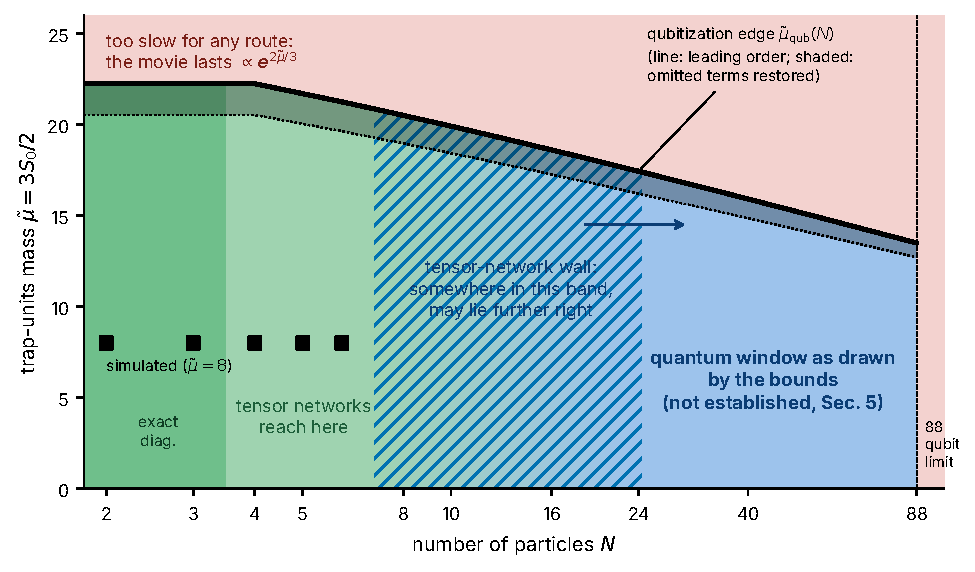
\includegraphics[width=0.8\textwidth]{figures/fig_regime.pdf}
\caption{\textbf{The window as the cost models draw it (and why it should not be read as a result about the dynamics).} Cluster size $N$
against the trap-units mass $\mut=3S_0/2$ (the tunneling time grows as $e^{2\mut/3}$). The curve is the qubitization edge of the leading-order cost model of \emph{one evolution}; the grey
band below it shows where the edge moves when two omitted terms are restored. Exact diagonalization (dark green) fails by an exact count (Table~\ref{tab:walls}). The tensor-network wall (hatched, fading) lies
in the band that the three entropy-growth scenarios of Section~\ref{sec:larger} give: first failing $N=\num{wall_pess_grid}$--\num{wall_opt_grid} when the bond
dimension is charged as $2^{S}$, and $N=\num{wallchi_sat_grid}$ when the measured Schmidt rank is charged instead (Section~\ref{sec:walls}). It may lie further
right, because the entropy is measured only up to $N=\num{Nmax_measured}$; it prices the entanglement of the prepared state, most of which is present without tunneling
(Section~\ref{sec:static}). Squares: the points simulated at $\mut=8$. The label \emph{quantum window} marks where the cost models leave a gap; this report does not establish it. \textbf{Imaginary-time Monte Carlo is not drawn and is not excluded:} it is sign-free in this model and is the nearest classical rival; it could close part of the window (Section~\ref{sec:mc}).
Budgets: Table~\ref{tab:params}.}
\label{fig:regime}
\end{figure}

\paragraph{What is, and is not, hard.}
Two nearby settings are easy classically, and we do not claim otherwise. If a single light particle tunnels through a
heavy, static background, the background acts as a fixed potential (Born--Oppenheimer~\cite{bornoppenheimer1927}), the
problem is one-body, and its cost per time step does not grow with the size of the background. If the background
reacts only locally and the entanglement stays low, a matrix product state with small bond dimension
suffices~\cite{vidal2004,schollwock2011,schuch2008}. Neither applies to the cluster studied here: all $N$ particles have
the same mass and any of them can cross, so there is no timescale gap; the pair interaction acts between every pair that
shares a valley, so there is no short chain of neighbours; and the entanglement generated by real-time dynamics is not
bounded in advance~\cite{calabrese2005}. We therefore measure it (Section~\ref{sec:measured}) and read the
tensor-network wall off the measured growth. Nothing here is a hardness theorem.

\paragraph{What this report is.}
The report is a bounds-first answer to this question and ends as a negative result: the window of Fig.~\ref{fig:regime} is what the bounds draw, and it is not established as a statement about the dynamics. The bounds and the measurements stand
(Sections~\ref{sec:measured} and~\ref{sec:discussion}); what does not stand is the reading that they open a window for the dynamics.
We therefore looked at what the prepared state is made of, by computing the eigenlevels of the Hamiltonian and the weight of the
start on each (Section~\ref{sec:static}). For $N\le5$ the state is two eigenstates plus a dressing, most of its entanglement
is static, and, if that persists, the signal is a short sum of cosines of quantities that do not involve time. The tensor-network walls price that static entanglement; they do not show that the dynamics is hard. Section~\ref{sec:open} states what remains.

\subsection{Parameters and conventions}
\label{sec:params}

Every choice that enters the results is listed in Table~\ref{tab:params}; the model itself is defined in
Section~\ref{sec:model}. Particles are distinguishable (labelled, like different isotopes), which is the worst case for the
classical side. Entropies are von Neumann entropies in bits. $\hbar=m=1$ in the simulations; $\mut$ is changed by
rescaling, never by changing the trap.

\begin{table}[ht]
\centering
\footnotesize
\caption{Parameters of the model, of the numerical representations and of the budgets. All values are read from the single configuration file of the simulations. The trap, the interaction and the budgets are choices, not fits; Appendix~\ref{app:choice} says why these values were chosen and Appendix~\ref{app:numerics} what each numerical setting controls.}
\label{tab:params}
\begin{tabular}{L{2.4cm}L{7.4cm}L{4.4cm}}
\toprule
Group & Quantity & Value \\
\midrule
Trap & barrier strength $A$, $U=A(x^2-1)^2+\tfrac12\omega_y^2y^2$ & $8$ \\
 & transverse $\omega_y^2$ & $2$ \\
Pair potential & Lennard-Jones $\epsilon$, $\sigma$, cap $V_{\rm cap}$ & $2$, $0.18$, $100$ \\
Particles & tilt $c+c_i$, offsets $c_i=(i-1)C_0$, $C_0$ & $0.15$; $c$ at resonance \\
 & mass, $\hbar$ (simulation units) & $1$, $1$ \\
Grid (basis 1) & cells $n_x\times n_y$, $M$; $\Delta x$, $\Delta y$ & $40\times30$, $1200$; $0.125$, $0.200$ \\
Modes (basis 2) & modes per particle $k$ (local dimension $d$) & $12$, $16$, $20$ \\
Qubits (basis 3) & qubits per particle $n_p$; auxiliary & $11$; $30$ \\
Starts & correlated: penalty $W$ on the wrong side & $30$ \\
Dynamics & Chebyshev propagation; window $T$; snapshot spacing $\Delta t$ (one protocol for all $N$) & $200$; $1.0$ ($201$ snapshots) \\
Working point & trap-units mass $\mut_0$; action $S_0$; switching time $t_0$ & $8$; $5.33$; $16.5$ \\
Budgets & memory $\Bmem$; compute $\Bflop$ & $\ensuremath{10^{12}}$ B; $\ensuremath{10^{20}}$ operations \\
 & logical qubits $\BQ$; T-gates $\BT$; precision $\varepsilon$ & $1000$; $\ensuremath{10^{12}}$; $\ensuremath{10^{-3}}$ \\
Cost models & Krylov vectors $v$; sweeps (compute prefactor $A_{\rm sw}$) & $10$; $100$ ($200$) \\
\bottomrule
\end{tabular}
\end{table}


\subsection{Findings in brief}
\label{sec:findings}

\begin{enumerate}[itemsep=0.2em]
\item \textbf{Exact methods and Monte Carlo.} Full-state storage is exponential in $N$ \stE{}. Real-time path sampling suffers the sign problem; imaginary-time Monte Carlo is sign-free in this model, is not excluded and is the nearest classical rival (Section~\ref{sec:mc}).
\item \textbf{Tensor networks.} Every layout pays $\chi\ge2^{S}$ for the entropy of a balanced cut \stE{}. The central-cut entropy was measured for
  $N=2$--\num{Nmax_measured} and grows by less per added particle than pair counting predicts (Fig.~\ref{fig:entropy}). A correlation graph reproduces the entropy of every subset to
  within \num{graph_maxdev} bit and picks the best layout \stM{}. Its pair weights fall roughly as $1/(N-1)$, as if the one-particle entropy were shared among the partners; this is
  a description of $N\le6$, not a derivation (Section~\ref{sec:graph}).
\item \textbf{Quantum route.} A leading-order qubitization count for \emph{one evolution} fits the budgets with room to spare and gives a mass edge that falls slowly with $N$ \stM{} (Section~\ref{sec:quantum}).
\item \textbf{The start is two levels plus a dressing} (Fig.~\ref{fig:spectrum}). For $N\le5$ the correlated start sits on two eigenstates (all particles in the crowded valley; one particle moved), with
  weight $B_2$ that falls with $N$ at fixed basis and rises with the basis size (Table~\ref{tab:static}, Fig.~\ref{fig:dressing}a). The rest lies within a few $J$ of the pair
  (Fig.~\ref{fig:dressing}b). An exact reflection symmetry removes the other levels (Fig.~\ref{fig:parity}).
\item \textbf{Most of the entropy is static.} Away from resonance, with no tunneling, the central entropy at $N=5$ is \num{off_Snat} bit against \num{Snat_N5} bit on resonance (Section~\ref{sec:static}).
  The tensor-network walls of Section~\ref{sec:walls} therefore price the isomers, not the transfer.
\item \textbf{A conditional reduction and an open question.} If the start stays in the span of the two states and a few sidebands, the signal is a sum of at most $(M+2)(M+3)/2$ cosines of static
  quantities, and the bond dimension is at most $(M+2)\chi_0$ (Proposition~\ref{prop:cond}). Whether $M(N)$ stays small is open; at fixed trap depth the regime itself ends near $N\approx\num{fu_Ntop_lo}$--\num{fu_Ntop_hi}
  (Fig.~\ref{fig:tilt}).
\item \textbf{The window} is therefore not established as a statement about the dynamics. It remains a statement about the price of one evolution on one side and of the static entanglement on the other.
\end{enumerate}

\paragraph{Status of statements.} \stE{} marks an identity or count; \stM{} a result derived under a stated model or measured with stated
parameters; \stC{} a result true if a named growth hypothesis holds. Section~\ref{sec:open} lists what is open. Appendix~\ref{app:choice} explains the choice of the model parameters, Appendix~\ref{app:proofs} holds the proofs,
Appendix~\ref{app:numerics} the numerical details and the raw logs behind each figure, Appendix~\ref{app:static} the spectrum of the start (method, one table of all cases, structural checks), and Appendix~\ref{app:quantum} the quantum cost model.

\section{The model and the task}
\label{sec:model}

This section defines the smallest system that shows the process we care about, the one parameter that controls it, and the quantity a simulator has to produce. We need a process in which a cluster switches between two arrangements by tunneling, a timescale for that switch, and an observable that records it; every cost in later sections is the cost of producing that observable up to that time.

\begin{figure}[t]
\centering
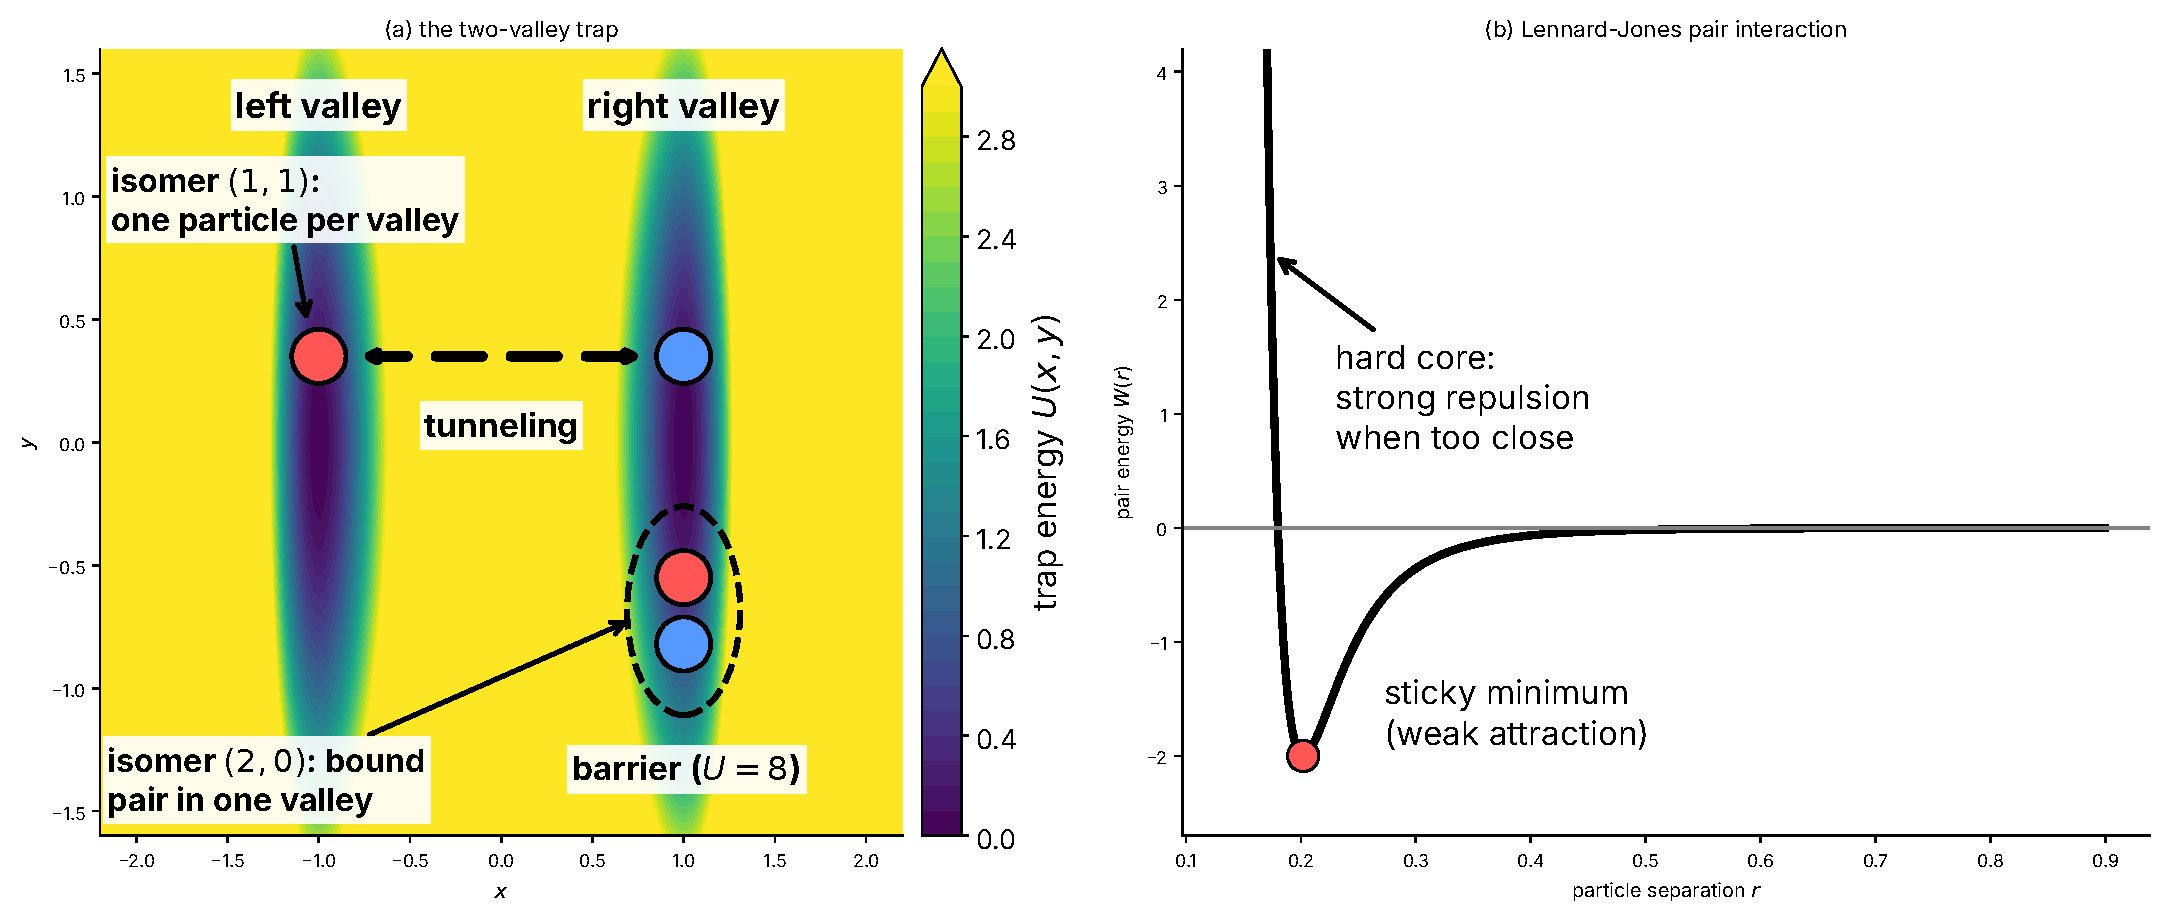
\includegraphics[width=0.95\textwidth]{figures/fig_model.pdf}
\caption{\textbf{The model.} (a) The two-valley trap (colour scale clipped at $U=3$, so the barrier, of height $U=A=8$,
appears uniformly bright), the two isomers of a two-particle cluster and the tunneling path between them.
(b) The capped Lennard-Jones pair interaction: hard core at short range, a shallow minimum at $r_{\min}$.
Parameters: Table~\ref{tab:params}.}
\label{fig:model}
\end{figure}

\paragraph{System.}
Each particle moves in two dimensions in a trap with two valleys, $U(x,y)=A(x^2-1)^2+\tfrac12\omega_y^2y^2$ (Fig.~\ref{fig:model}a): the valleys lie at $x=\pm1$ and are separated
by a hill of height $A$ that a particle cannot climb but can tunnel through. A tilt $c\,x$ added to each particle makes one valley deeper. Two particles at
distance $r$ repel at short range and attract weakly at long range through the Lennard-Jones potential $W(r)=4\epsilon[(\sigma/r)^{12}-(\sigma/r)^{6}]$, capped at $V_{\rm cap}$
(Fig.~\ref{fig:model}b). The interaction range is small compared with the valley separation, so particles interact only
when they share a valley, and the cluster is described by \emph{how many particles sit in which valley}: the occupation isomers,
$(1,1)\leftrightarrow(2,0)$ for two particles, $(N-1,1)\leftrightarrow(N,0)$ in general. The Hamiltonian is the sum of the kinetic energy, the trap, the tilt and the pair interactions,
\begin{equation}
\hat H_N(c)=\sum_{i=1}^{N}\Big[-\tfrac12\nabla_i^{2}+U(x_i,y_i)+(c+c_i)\,x_i\Big]+\sum_{i<j}W(|\mathbf r_i-\mathbf r_j|),
\qquad c_i=(i-1)C_0 .
\label{eq:HN}
\end{equation}
The tilt is tuned to the \emph{resonant} value $c^*(N)$ at which the two isomers have the same energy; they then mix completely and tunneling between them is fastest. The small offsets $c_i$ make
the particles non-identical (labelled, like different isotopes), which is the harder case for classical methods. The observable is the number of particles in the right valley,
\begin{equation}
\hat O=\sum_{i=1}^{N}\Theta(x_i),\qquad \|\hat O\|=N .
\label{eq:Oobs}
\end{equation}
It changes by one when one particle crosses the barrier, so it is the direct readout of the isomer switch. On the grid one column lies exactly on the barrier top; it counts with weight $\Theta(0)=\tfrac12$, so the two valleys are treated alike (Appendix~\ref{app:numerics}).

\paragraph{The one knob.}
Rescaling lengths by $\sigma$ and energies by $\epsilon$ leaves one dimensionless mass, $\muq=m\sigma^2\epsilon/\hbar^2$. What matters for tunneling is not the mass itself but how heavily it weighs on the barrier: the \emph{action under the barrier}
$S_0=\tfrac43\sqrt{2mA}\,a/\hbar$ ($a=1$ the half-separation of the valleys), and the tunneling time grows as $e^{S_0}$~\cite{helffer1984,garg2000}. We therefore use the \emph{trap-units} mass $\mut:=\tfrac32S_0$, for which the tunneling time grows as $e^{2\mut/3}$.
The simulations run at one light point, $\mut=\num{mut0}$
($S_0=\num{Szero}$, $\muq=\num{muzero}$), where one isomer transfer takes $t_0=\num{tstar0}$ (the two-particle switching time $\pi/\dE_2$ measured on the position grid; Appendix~\ref{app:numerics}). In an optical lattice of depth $s$ recoil energies the barrier action is $S_0=2\sqrt s$ for every
species, so $\mut=3\sqrt s$ and the mass drops out of the single-particle part of the tunneling time (Appendix~\ref{app:proofs}); this is
a statement about the single-particle action only, since the pair-interaction cost of Appendix~\ref{app:quantum} differs between species.

\paragraph{The task.}
In words: start the cluster in one arrangement, let it evolve, and report how many particles are in the right valley as a function of time, with a stated accuracy, until the first full transfer. A simulator that can do this has reproduced the tunneling.
\begin{defn}[Task]\label{def:task}
Given a valley-localized start $\psi_0$, approximate $f(t)=\langle\psi_0|e^{i\hat H_Nt}\Op\,e^{-i\hat H_Nt}|\psi_0\rangle$ for $0\le t\le\Tobs$ to additive error
$\varepsilon\|\Op\|$.
\end{defn}
For a clean doublet (two levels well separated from all others) of splitting $\dE_N$ the observation time is the first isomer transfer, $\Tobs=\pi/\dE_N$; where no clean doublet exists we use the
first minimum of $\langle\Op\rangle(t)$. The cost of a quantum simulation grows with $\Tobs$, so we need $\Tobs$ at masses other than the simulated one. With the semiclassical dependence on the barrier action, anchored to the measured two-particle value,
\begin{equation}
\Tobs(N,\mut)=g_N\,t_0\,e^{2(\mut-\mut_0)/3}\Big(\frac{\mut_0}{\mut}\Big)^{1/2},\qquad g_N=\frac{\dE_2}{\dE_N}.
\label{eq:Tobs}
\end{equation}
The factor $g_N$ says how much slower the $N$-particle transfer is than the two-particle one. Equation~\eqref{eq:Tobs} is an interpolation anchored to a measurement, not an ab-initio law; at $S_0=\num{Szero}$ the asymptotic regime is not reached. The gap ratio $g_N$ enters the quantum
price linearly (a ratio $g_N>1$ lowers the quantum edge by $\tfrac32\ln g_N$). We carry $g_N=1$ and test it where a clean doublet exists
(Appendix~\ref{app:numerics}).

\paragraph{Representations and starts.}
The same $\hat H_N$ can be written in three ways, and each route of Section~\ref{sec:framework} needs a different one (Table~\ref{tab:params}). \emph{Basis 1}, the position grid, has $d=M=\num{M_grid}$ cells per particle and $d^N$ amplitudes; the exact-storage count and the cost models refer to it. \emph{Basis 2}, the mode basis, keeps the lowest $k$ eigenstates of each particle's own one-particle Hamiltonian
($d=k$); all entanglement measurements use it, because the grid state does not fit in memory beyond $N=3$. Its price is truncation of the correlation hole between particles
that share a valley, so every mode-basis entropy is quoted with its spread over $k$. \emph{Basis 3}, the qubit register, is the grid written in binary,
$n_p=\lceil\log_2M\rceil=\num{n_p}$ qubits per particle; it is used only to count quantum cost, and no quantum computation is simulated.
Two starts are used. The \emph{product start} is a product of one-particle valley orbitals; it ignores the correlation hole between particles in the same valley, which
makes it a quench for $N\ge3$. The \emph{correlated start} is the ground state of $\hat H_N+W\sum_iP^{\rm wrong}_i$ with a penalty of strength $W$ (not the pair energy $W(r)$) on the wrong side for each particle; it
contains the pair correlation and is the physically relevant isomer. Preparing it on a quantum computer costs extra, which the quantum price of Section~\ref{sec:quantum} does not include.
All entropy results below are for the correlated start unless stated.

\section{Framework: one inequality per route}
\label{sec:framework}

Each of the four standard ways of simulating the dynamics is limited by one resource: memory for exact methods, entanglement for tensor networks, statistical noise for Monte Carlo and gate count for a quantum computer
(Table~\ref{tab:routes}). For every route this section says in words what it stores or samples and what limits it, and then writes the limit as an inequality \emph{cost}$(N)\le$\emph{budget}. The first $N$ at which
the inequality fails is the \emph{wall} of the route. Writing the inequalities before any measurement shows which statements are arithmetic, which depend on a model, and which depend on a quantity that must
be measured (the entanglement, Section~\ref{sec:measured}). Let $d$ be the local dimension per particle ($d=M$ on the grid, $d=k$ in the mode basis), so that the full state has $d^N$ amplitudes. Budgets and values are in Table~\ref{tab:params};
proofs are in Appendix~\ref{app:proofs}.

\begin{table}[t]
\centering
\footnotesize
\caption{The four routes: what each one stores or samples, which resource limits it, and what has to be known to evaluate the limit. The status marks are those of Section~\ref{sec:intro}.}
\label{tab:routes}
\begin{tabular}{@{}p{0.17\textwidth}p{0.24\textwidth}p{0.23\textwidth}p{0.27\textwidth}@{}}
\toprule
route & stores or samples & limited by & needs, to be evaluated \\
\midrule
1.\ exact diagonalization & all $d^N$ amplitudes of the state & memory & nothing: a count \stE{} \\
2.\ tensor networks & a chain of small tensors joined by bonds & bond dimension, set by the entanglement across the cut of the chain & the cut entropy as a function of $N$: measured up to $N=\num{Nmax_measured}$, then a model \stM{}\,\stC{} \\
3.\ Monte Carlo & random paths & statistical noise (cancellation of path weights, absent in imaginary time) & imaginary time (the right variant): the static spectrum, open \\
4.\ quantum computer & $\lceil\log_2 d\rceil$ qubits per particle & qubits and T gates, set by the evolution time & the observation time $\Tobs$ and the norm of $\hat H_N$ \stM{} \\
\bottomrule
\end{tabular}
\end{table}

\subsection{Route 1: exact diagonalization}

Exact methods store the whole wave function, one complex number per configuration of the $N$ particles, and diagonalize $\hat H_N$ or propagate the vector. The memory is therefore a count.

\begin{prop}[Memory of full-state methods]\label{prop:ed}\stE{}
Storing $v$ complex vectors of $N$ particles with local dimension $d$ needs $16\,v\,d^N$ bytes. Full-state diagonalization or Krylov propagation therefore exceeds $\Bmem$ for
$N>\NED(d):=\lfloor\ln(\Bmem/16v)/\ln d\rfloor$.
\end{prop}
The count is basis-dependent (on the grid it concerns the position basis; in a mode basis the same formula gives a later wall, Table~\ref{tab:walls}) and says nothing about methods that do not store the full state.

\subsection{Route 2: tensor networks}
\label{sec:fw-tn}

\paragraph{The idea.}
A tensor network writes the state of $N$ particles not as one array with $d^N$ entries but as a chain of small tensors, one per particle, each joined to its neighbours by a \emph{bond}~\cite{white1992,vidal2004,schollwock2011,paeckel2019}. In the chain form, a \emph{matrix-product state}, the number of
values a bond carries is the \emph{bond dimension} $\chi$. The memory is then of order $N d\chi^2$ and one time step costs of order $N(d\chi)^3$ operations, linear in $N$ instead of exponential, provided $\chi$ stays small. Everything depends on how large $\chi$ must be.

\paragraph{The cut.}
A bond of the chain splits the particles into two groups: those to its left, $A=\{1,\dots,b\}$, and the rest. We call this split the \emph{MPS cut}. Whatever the left group has in common with the right group must pass through that one bond. The amount
that has to pass is the entanglement between the two groups: writing the state as a sum of products of a left state and a right state (a Schmidt decomposition), the number of terms is the Schmidt rank, and a bond that carries fewer values cannot represent the state. The entanglement entropy $S_A$ of the cut, in bits, is the logarithm of the effective number of terms, so the bond must have dimension of at least $2^{S_A}$.
The cost of the simulation is therefore set by the \emph{largest cut entropy} that the state reaches during the evolution: low where the two groups are nearly independent, high where they are strongly correlated. After a sudden change the entropy typically grows with time~\cite{calabrese2005}, and matrix-product simulations stop being possible when it becomes large~\cite{schuch2008}. The same state can be cheap or expensive depending on how the particles are ordered along the chain (a tree-shaped network is a different choice of cuts).

\paragraph{How we measure it.}
We compute the state exactly for $N=2$--$\num{Nmax_measured}$ (Section~\ref{sec:measured}), evaluate $S_A(t)$ for the cuts of interest at every time step, keep the largest value over the observation time, and take the largest of these over the bonds of the chain. This number, $\SN$ below, is the input of the cost.
The measurements cannot reach the sizes where a wall would sit, so Section~\ref{sec:larger} extends them with a model, and this subsection supplies only the formulas that turn an entropy into a cost.

\paragraph{Cuts and layouts.}
For a subset $A$ of $a$ particles let $S_A(t)$ be the entropy in bits of $\psi(t)$ across $A\,|\,A^c$, and $\sigma(A)=\max_{0\le t\le\Tobs}S_A(t)$. A matrix-product state in the order $1,\dots,N$
has the $N-1$ prefix cuts $A_b=\{1,\dots,b\}$; a tree has a different set. Three numbers summarize the task:
\begin{equation}
\Snat:=\max_{1\le b<N}\sigma(A_b),\qquad
\Sperp:=\min_{\lceil N/3\rceil\le|A|\le\lfloor N/2\rfloor}\sigma(A),\qquad
\Smax:=\max_{|A|=\lfloor N/2\rfloor}\sigma(A).
\label{eq:threeS}
\end{equation}
$\Snat$ is what the natural-order matrix-product state pays; $\Sperp$ is what \emph{every} tree layout of node degree at most three pays, because every such tree has a bond with
$\lceil N/3\rceil\le a\le\lfloor N/2\rfloor$ particles on its smaller side (Lemma~\ref{lem:pivot}); $\Smax$ is the worst balanced layout. Since $\Sperp\le\Snat\le\Smax$, the bracket
$[\Sperp,\Smax]$ is the layout uncertainty, and we write $\SN:=\Snat$.

\begin{prop}[Tensor networks]\label{prop:tn}
\emph{(a)}\ \stE{} A tensor network that represents $\psi(t)$ exactly has bond dimension $\chi\ge2^{S_A(t)}$ on every bond that cuts off $A$; a matrix-product state needs
$\chi\ge2^{\Snat}$ at some bond and any tree of degree $\le3$ needs $\chi\ge2^{\Sperp}$ at some bond.\\
\emph{(b)}\ \stE{} $S_A\le\min(a,N-a)\log_2d$, and $S_A\le\sum_{i\in A}S_{\{i\}}$ (Lemma~\ref{lem:cap}).\\
\emph{(c)}\ \stM{} With $\chi=2^{\SN}$ on every bond the memory is $16\,N\,d\,\chi^2$ bytes and a time evolution costs $A_{\rm sw}N(d\chi)^3$ operations.\\
\emph{(d)}\ \stC{} For any non-decreasing law $\SN=S(N)$ the model of (c) exceeds a budget for $N>\NTN:=\lfloor\min(N^*_{\rm flop},N^*_{\rm mem})\rfloor$, with
\begin{equation}
3\,S(N^*_{\rm flop})+\log_2N^*_{\rm flop}=\log_2\frac{\Bflop}{A_{\rm sw}d^{3}},\qquad
2\,S(N^*_{\rm mem})+\log_2N^*_{\rm mem}=\log_2\frac{\Bmem}{16\,d}.
\label{eq:Nstar}
\end{equation}
\end{prop}
In words: (a) is the statement above, that the bond must carry $2^{S}$ values; (b) says the entropy cannot exceed what the smaller side can hold or the sum of the single-particle entropies, so it cannot be arbitrarily large; (c) turns $\chi$ into memory and time; (d) asks at which $N$ these exceed the budgets, which needs the law $S(N)$.

\paragraph{The growth law is an input, not a result.}
To find the wall we need $\SN$ as a function of $N$, and the data reach only $N=\num{Nmax_measured}$. Nothing in $\hat H_N$ alone fixes this dependence: adding a particle changes the Hamiltonian, and a permutation-symmetric preparation of the same family has
$\SN=O(\log N)$ at fixed $k$ (Remark~\ref{rem:symm}). Growth is a property of the task, Hamiltonian \emph{and} start, and must be measured. Two one-parameter laws, anchored at a measured
$N_{\rm ref}$, are the usual candidates:
\begin{align}
H_S(s):&\quad S(N)=S_{\rm ref}+s\,(N-N_{\rm ref}), &&\text{constant growth per added particle,}\label{eq:HS}\\
H_P(\beta):&\quad S(N)=S_0+\beta\,\pairs(N),\ \ \pairs(N)=\lfloor N/2\rfloor\lceil N/2\rceil, &&\text{constant weight per crossing pair.}\label{eq:HP}
\end{align}
(Here $s$ counts bits per added particle, not the optical-lattice depth, and $S_0$ is a fitted entropy offset, not the tunneling action; both are defined in Section~\ref{sec:model}.)
Under $H_S(s)$ Eq.~\eqref{eq:Nstar} gives
\begin{equation}
N^*_{\rm flop}=N_{\rm ref}+\frac{\log_2\!\big(\Bflop/A_{\rm sw}d^{3}\big)-\log_2N^*_{\rm flop}-3S_{\rm ref}}{3s},
\label{eq:Nflop}
\end{equation}
and the memory analogue. Three consequences hold for every measured input: the wall moves as $1/s$; it moves by $\log_2f/(3s)$ particles for a factor $f$ in the compute budget
or in the sweep count; and it disappears if $\SN$ saturates ($s\to0$). Section~\ref{sec:graph} explains which of the two laws the data follow and why: the correlation-graph picture contains
both as two normalizations of the same graph.

\paragraph{What is and is not a bound.}
(a)--(b) are identities for an \emph{exact} representation. A representation truncated at discarded weight $\epsilon$ (not the well depth) needs the numerical Schmidt rank $\chi(\epsilon)$, which is not ordered
with $2^S$ in general~\cite{schuch2008}. For this task it lies above (Section~\ref{sec:seed}), so charging $2^{\SN}$ understates the cost. In the other direction the model charges the
central $\chi$ on every bond although the bond profile is concave (Lemma~\ref{lem:chord}). $\NTN$ is therefore a resource estimate for exact-in-$\chi$ matrix-product states of the task, not an
impossibility statement for tensor-network dynamics.

\subsection{Route 3: Monte Carlo}
\label{sec:mc}

\paragraph{The idea.}
Monte Carlo estimates a sum over very many terms by averaging a random sample of them; the statistical error falls as $1/\sqrt\nu$ for $\nu$ samples, whatever the dimension. For quantum dynamics the sum is over paths of the particles~\cite{ceperley1980}, and it works as long as the path weights do not cancel. In real time they are phases and do cancel (the sign problem~\cite{troyer2005,muhlbacher2008}): for the straightforward absolute-value path estimator the sample count satisfies $\ln\nu\ge2N\Gamma_\infty t/\hbar-N\ln M+2\ln(1/\varepsilon)$ with $\Gamma_\infty=\frac{\pi^2\hbar^2}{3m\,\Delta x^2}(1-M^{-2})$ per direction~\cite{trefethen2000}, so real-time sampling is simply not the right Monte Carlo for this task. The right one works in imaginary time.

\paragraph{Imaginary-time Monte Carlo is the route that may work, and this report does not exclude it.} Replacing the real time $t$ by an imaginary time $-i\tau$ turns the phase $e^{-i\hat Ht}$ into the damping $e^{-\tau\hat H}$. The model has distinguishable particles and a local potential, so there are no exchange signs and every path weight is positive: path-integral and diffusion Monte Carlo~\cite{ceperley1980,anderson1975} sample it without cancellation, and the sign problem of the previous paragraph does not arise. What such a method returns is not the movie but \emph{static} quantities: energies, including tunneling splittings~\cite{sindzingre1989,richardson2011}, and correlation functions $C(\tau)=\langle\psi_0|\hat O\,e^{-\tau(\hat H-E_0)}\hat O|\psi_0\rangle=\sum_n|c_n|^2e^{-\tau(E_n-E_0)}$ whose decay carries the levels $E_n$ and their weights $|c_n|^2$ in the start.

\paragraph{How the signal would follow.} If the start lies on two eigenstates, the signal is $\langle\Op\rangle(t)=a+b\cos(\Delta E\,t+\varphi)$: the splitting comes from imaginary-time data, the weights from the decay of a start-state correlator, and no real-time simulation is needed. This is the situation at $N=2,3$ and at $N=4$, $k=20$ (Table~\ref{tab:mc}), and it is the picture that Section~\ref{sec:static} supports for $N\le5$, in the sense that two levels carry most of the start. Where the gated pair is not the pair that carries the weight, a cosine at its splitting explains none of the signal, and the signal has several frequencies whose number grows with $N$ (Fig.~\ref{fig:cosines}); a prediction then needs a handful of gaps and weights, the sidebands of Proposition~\ref{prop:cond}, from imaginary-time data. Two things could make this work: the dressing may be close to Gaussian (a spin--boson problem), in which case the weights follow from a few harmonic quantities of the two isomers (the Huang--Rhys test of Section~\ref{sec:open}); and estimators built from correlation functions of several trial states could give the few low levels that matter without the whole spectrum. Neither is tested here.

\paragraph{What could make it fail.} Recovering a sum of exponentials from imaginary-time data is an ill-conditioned inverse problem whose difficulty grows with the number of terms~\cite{jarrell1996}, and the number of cosines needed grows with $N$. Whether the few-level description survives in a converged basis for larger clusters is the open problem of Section~\ref{sec:openproblem}. Until it is measured, imaginary-time Monte Carlo is the nearest classical rival to a quantum computer here, and the window of Fig.~\ref{fig:regime} does not account for it.

\subsection{Route 4: quantum simulation}

A quantum computer stores the grid state of each particle in $n_p=\lceil\log_2 d\rceil$ qubits, so the register grows linearly in $N$, and applies $e^{-i\hat H_Nt}$ as a circuit. In the fault-tolerant setting the cost that matters is the number of T gates. Qubitization~\cite{low2019qubitization} makes a number of calls to a block-encoding of $\hat H_N$ that is proportional to the product of the evolution time $\Tobs$ and the one-norm $\lambda$ of the Hamiltonian (the sum of the sizes of its terms); product formulas~\cite{childs2021trotter} are the alternative (Appendix~\ref{app:quantum}). Because the tunneling time grows as $e^{2\mut/3}$ (Section~\ref{sec:model}), the question for this route is not whether an evolution fits at the simulated mass but up to which mass it still fits: the \emph{mass edge} $\mutq(N)$.

\begin{prop}[Quantum resources]\label{prop:q}\stM{} (leading-order counts, not compiled circuits)\\
\emph{(a)} Qubits: $Q(N)=N\,n_p+b_0$, with $b_0$ the arithmetic workspace and control qubits; the budget allows $N\le\NQ:=\lfloor(\BQ-b_0)/n_p\rfloor$.\\
\emph{(b)} Qubitization: with one-norm $\lambda(N)=N\lambda_U+\binom N2\lambda_W$ the number of block-encoding queries is $\lceil\lambda(N)\Tobs+\ln(1/\varepsilon)\rceil$, each costing $C_{\rm sel}$
T-gates, so $T_{\rm qub}\le\BT$ exactly when $\mut\le\mutq(N)$,
\begin{equation}
\mutq(N)=\mut_0+\tfrac32\ln\!\Big[\frac{X}{g_N\,\lambda(N)\,t_0}\Big]+\tfrac34\ln\frac{\mutq(N)}{\mut_0},\qquad X=\frac{\BT}{C_{\rm sel}}-\ln\frac1\varepsilon .
\label{eq:muqub}
\end{equation}
\end{prop}
Two properties carry the paper's quantum claims. The edge is \emph{logarithmic in the budget}: $\partial\mutq/\partial\ln\BT\simeq\tfrac32$, so a thousandfold larger gate budget moves it by
about $\num{mu_budget_shift}$. And it is \emph{slow in $N$}: when the pair term dominates, $\lambda\simeq\tfrac12N^2\lambda_W$ and $\mutq(N)\simeq\mutq(N_0)-3\ln(N/N_0)$. The Trotter edge, and what the model omits,
are in Appendix~\ref{app:quantum}.

\subsection{The window}
\label{sec:window}

The window is the set of sizes and masses where every classical route has failed and the quantum route still fits. Its lower edge in $N$ comes from the classical walls, in practice the tensor-network wall, because the exact count is not binding on our grid; its upper edge in mass is the quantum edge. Whether the window exists therefore depends on how fast the entropy grows: if it grows slowly, the tensor-network wall lies beyond the quantum register and the window is empty.

\begin{defn}[Window]\label{def:window}
For a model instance $\mathcal M$, budgets $\mathcal B=(\Bmem,\Bflop,\BQ,\BT,\varepsilon)$ and a growth law $S(\cdot)$, the \emph{window} is
\[
\Win(\mathcal M,\mathcal B;S)=\big\{(N,\mut):\ N>\NED,\ N>\NTN[S],\ N\le\NQ,\ \mut\le\mutq(N)\big\}.
\]
Imaginary-time Monte Carlo is not part of the definition; it is a rival that the window does not price (Section~\ref{sec:mc}).
\end{defn}
The window is non-empty at a mass $\mut$ exactly when $\NTN<N_{\rm hi}(\mut):=\min\{\NQ,\max\{N:\mutq(N)\ge\mut\}\}$. In terms of a constant growth $s$ anchored at $(N_{\rm ref},S_{\rm ref})$, Eq.~\eqref{eq:Nflop} solved for $s$ gives
\begin{equation}
s>s_{\rm crit}(N_{\rm hi})=\frac{\log_2\!\big(\Bflop/A_{\rm sw}d^3\big)-\log_2N_{\rm hi}-3S_{\rm ref}}{3\,(N_{\rm hi}-N_{\rm ref})}.
\label{eq:scrit}
\end{equation}
``Is there a window?'' is therefore answered by comparing the growth with $s_{\rm crit}$, and ``where does it begin?'' by Eq.~\eqref{eq:Nflop}; the first has a robust answer and the second a soft one.

\section{What the simulations show}
\label{sec:measured}

This section reports what exact propagation gives for $N=2$--$\num{Nmax_measured}$ and what it implies for the tensor-network cost. Three things are measured: the tunneling signal $\langle\Op\rangle(t)$ (does the cluster oscillate coherently between its two arrangements?), the entanglement entropy across cuts of the particle order (the MPS cut of Section~\ref{sec:fw-tn}, whose entropy sets the bond dimension and hence the cost, Eq.~\eqref{eq:Nstar}), and a correlation graph that describes the entropies and lets them be carried to larger $N$. All numbers are in Table~\ref{tab:measured}; the text discusses what they show. The runs use the correlated start, the mode basis with $k=12$ unless a $k$ is named, and the resonant tilt of each $N$ (Table~\ref{tab:params}, Appendix~\ref{app:numerics}).

\paragraph{What is observed.}
\begin{itemize}[itemsep=0.15em]
\item The signal is a clean oscillation at $N=2,3$ and irregular from $N=4$ on.
\item The central-bond entropy grows with $N$, but by less per added particle than pair counting predicts; the choice of particle order changes it little, and the choice of start changes it a lot.
\item A correlation graph whose edge weights are the one-particle entropy shared among the partners reproduces every measured entropy and rules out the pair-counting law at $N=5,6$.
\item Carried beyond $N=\num{Nmax_measured}$ the graph gives a range of scenarios (Table~\ref{tab:scen}) but no measurement; Section~\ref{sec:static} shows that most of the entropy is present without any tunneling.
\end{itemize}

\subsection{The signal and the cut entropies}
\label{sec:signal}
\label{sec:seed}

\begin{figure}[t]
\centering
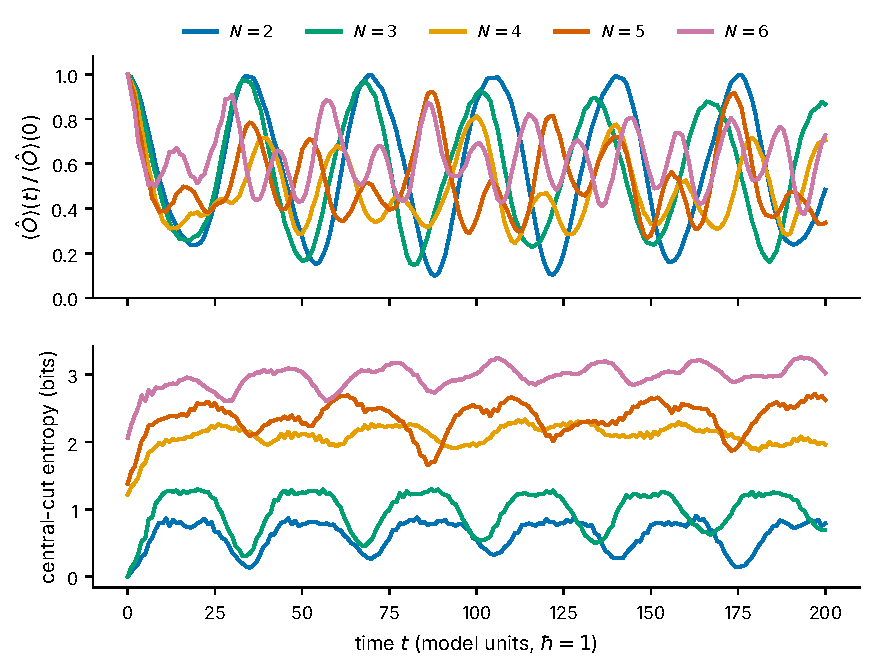
\includegraphics[width=0.78\textwidth]{figures/fig_signal.pdf}
\caption{\textbf{The tunneling signal and its entanglement.} Top: the number of particles in the right valley, normalized to its initial value, for the correlated start at the resonant tilt.
Bottom: entropy across the central bond of the particle order, in bits. Source: the time series stored with each run (Appendix~\ref{app:numerics}).}
\label{fig:signal}
\end{figure}

\begin{table}[!tp]
\centering
\small
\caption{Everything measured on the simulated runs, by cluster size ($k=12$ modes per particle, correlated start at the resonant tilt, one protocol for every $N$: maximum over $[0,T]$ with $T=\num{Tprot}$, snapshot spacing $\num{dtsnap}$; entropies in bits). \emph{Signal} (Fig.~\ref{fig:signal}): lowest value of $\langle\Op\rangle/\langle\Op\rangle(0)$ in the window; largest value after it first falls below $\tfrac12$ (a clean oscillation returns to about one); weight of the start on the gated pair of levels (Table~\ref{tab:start}); time of the central-bond maximum. \emph{Cut entropies} (Eq.~\eqref{eq:threeS}): mean one-particle entropy $\bar S_1$; best balanced, natural-order and worst balanced cut; $\Snat$ is the central bond; numerical Schmidt rank $\chi$ of the central bond at discarded weight $10^{-3}$. \emph{Growth}: increments with each added particle. \emph{Layout}: how much more the worst order pays than the best; how much more the order chosen on the graph pays than the exact optimum; rank correlation between graph and exact costs over all orders. \emph{Graph} (Section~\ref{sec:graph}): mean edge weight $w_{ij}$ against the sharing-law weight $2\bar S_1/(N-1)$ of Eq.~\eqref{eq:sharing}, and the sharing-law central cut against the measured one. \emph{Laws fitted to $N\le4$}: excess of the pair-counting and of the linear law over the measured central bond. \emph{Start}: central bond for the product start (a quench; no run exists for $N\ge5$), to be compared with $\Snat$. A dash marks a quantity that does not exist for that $N$ (an increment, a rank correlation over one order, a fit at the fitted sizes) or a run that was not made.\num{d45_note}}
\label{tab:measured}
\begin{tabular}{lrrrrr}
\toprule
$N$ & 2 & 3 & 4 & 5 & 6 \\
\midrule
\multicolumn{6}{l}{\emph{Signal}} \\
lowest value of $\langle\Op\rangle/\langle\Op\rangle(0)$ & 0.10 & 0.15 & 0.25 & 0.27 & 0.37 \\
largest value after the first fall below $\tfrac12$ & 1.00 & 0.97 & 0.81 & 0.92 & 0.90 \\
weight of the start on the gated pair & 0.98 & 0.94 & 0.46 & 0.35 & 0.31 \\
time of the central-bond maximum & 163 & 89 & 114 & 197 & 193 \\
\multicolumn{6}{l}{\emph{Cut entropies}} \\
$\bar S_1$ & 0.90 & 1.32 & 1.75 & 1.88 & 1.93 \\
best balanced cut $\Sperp$ & 0.90 & 1.29 & 2.33 & 2.62 & 2.88 \\
central bond $\Snat$ & 0.90 & 1.30 & 2.33 & 2.72 & 3.26 \\
worst balanced cut $\Smax$ & 0.90 & 1.37 & 2.54 & 2.93 & 3.70 \\
Schmidt rank $\chi(10^{-3})$ & 7 & 10 & 38 & 74 & 325 \\
$\chi(10^{-3})/2^{\Snat}$ & 3.7 & 4.1 & 7.5 & 11.3 & 34.0 \\
\multicolumn{6}{l}{\emph{Growth}} \\
increment of $\Snat$ & -- & 0.39 & 1.04 & 0.38 & 0.54 \\
increment of $\bar S_1$ & -- & 0.41 & 0.43 & 0.14 & 0.05 \\
\multicolumn{6}{l}{\emph{Layout}} \\
worst order minus best & 0.00 & 0.07 & 0.21 & 0.22 & 0.44 \\
graph-chosen order minus optimum & 0.00 & 0.00 & 0.02 & 0.00 & 0.00 \\
rank correlation, graph against exact & -- & 1.00 & 0.45 & 0.46 & 0.80 \\
\multicolumn{6}{l}{\emph{Graph}} \\
mean edge weight, measured & 1.81 & 1.49 & 1.24 & 1.00 & 0.86 \\
sharing-law weight & 1.81 & 1.32 & 1.16 & 0.94 & 0.77 \\
sharing-law central cut & 0.90 & 1.32 & 2.33 & 2.82 & 3.47 \\
\multicolumn{6}{l}{\emph{Laws fitted to $N\le4$: excess over the measured central bond}} \\
pair-counting law & -- & -- & -- & 0.57 & 1.47 \\
linear law & -- & -- & -- & 0.23 & 0.40 \\
\multicolumn{6}{l}{\emph{Start}} \\
central bond, product start (correlated start: $\Snat$ above) & 0.90 & 2.31 & 4.81 & -- & -- \\
\bottomrule
\end{tabular}
\end{table}


\paragraph{Signal.} At $N=2,3$ the observable falls to a small fraction of its initial value and returns almost completely: a clean oscillation of one particle between the valleys at a single splitting. From $N=4$ the lowest value is higher, the return is incomplete and the curves become irregular (Fig.~\ref{fig:signal}). The weight of the start on the gated pair of levels, the pair of smallest splitting that passes the doublet gates, drops with it; it measures the pair selector and the basis as much as the cluster, and the two levels that actually carry the weight give a different picture (Section~\ref{sec:static}). Where a clean doublet exists the ratio $g_N=\dE_2/\dE_N$ of Eq.~\eqref{eq:Tobs} lies between $\num{gN_lo}$ and $\num{gN_hi}$, which supports carrying $g_N=1$ in the quantum price; where it does not, the first minimum of $\langle\Op\rangle(t)$ defines $\Tobs$. The central-cut entropy rises within the first period and then oscillates; its maximum lies inside every window, but late at $N=2,5,6$, where it keeps creeping up with the window (Table~\ref{tab:protocol}).

\paragraph{Growth is not constant per particle.} The central bond grows unevenly, and by less per particle than pair counting predicts. The largest step is the one into $N=4$, the first size at which the $k=12$ basis does not hold a clean doublet (Table~\ref{tab:start}); how much of it belongs to the cluster and how much to the basis is not settled. The one-particle entropy saturates quickly, so the growth of the central bond is carried by the number of partners rather than by the entropy of each particle. The constant-growth law (Eq.~\eqref{eq:HS}) and the pair-counting law (Eq.~\eqref{eq:HP}) each have two parameters and can be made to pass through the points $N\le4$; they then disagree with each other and with the data at $N=5$ and $N=6$.

\paragraph{The layout matters little.} The best balanced cut $\Sperp$, the natural-order cut $\Snat$ and the worst balanced cut $\Smax$ differ by a small amount that grows with $N$. The natural order is among the best of all $N!/2$ orders at $N=3,\dots,6$, so $\SN=\Snat$ is the conservative-for-the-classical-side reading: the best order is already used.

\paragraph{The start matters a lot.} The product start ignores the correlation hole of particles that share a valley, so it is a quench that injects entropy, far above that of the correlated start already at $N=3,4$. Charging it would inflate the classical cost by a factor that grows with $N$; we use the correlated start, which is also the physical isomer.

\paragraph{Basis and compression.} The central entropy falls with $k$ at $N=4,5$, while the numerical Schmidt rank at discarded weight $10^{-3}$ rises (Table~\ref{tab:k}, Appendix~\ref{app:numerics}). The rank is far above $2^{S}$ and the ratio grows with $N$, so a matrix-product state that stores the state to this accuracy is more expensive than the $\chi=2^S$ of the cost model (Section~\ref{sec:walls}). Neither quantity is converged in $k$.

\subsection{The cut entropy is a cut of a correlation graph}
\label{sec:graph}

The entropies of Table~\ref{tab:measured} are well described by a graph on the particles whose edge weights are measured mutual informations.

\paragraph{The graph.}
Idea: the entropy across a cut is large when many particles on one side are strongly correlated with particles on the other. If we know how correlated each pair is, we can add up the correlation across the cut instead of computing the full entropy, and we can search for the particle order whose worst cut is cheapest. Quantitatively, let $I_{ij}(t)=S_i+S_j-S_{ij}$ be the mutual information (bits) between particles $i$ and $j$ and $w_{ij}=\max_tI_{ij}(t)$. For a pure state $S_A=\tfrac12I(A\!:\!A^c)$, so the natural estimate of the entropy across $A\,|\,A^c$ is
the weight of the cut edges,
\begin{equation}
C(A)=\tfrac12\sum_{i\in A,\ j\notin A}w_{ij}.
\label{eq:Cgraph}
\end{equation}
Choosing a matrix-product order is then choosing a linear order of the vertices that keeps the maximal prefix cut small (a weighted cutwidth), and choosing a tree is a carving problem (tree structures can also be optimized automatically from the measured entanglement~\cite{hikihara2023}); a balanced minimum cut is the lower bound that every layout pays and a balanced
maximum cut is the worst layout. Mutual-information graphs have been used to \emph{choose} the orbital order of density-matrix renormalization group
calculations~\cite{rissler2006,barcza2011,szalay2015}; the idea of reading an entropy as a cut is not new. For classical networks the maximum flow equals the minimum cut~\cite{dantzig2003max}; in continuum geometries the largest flux of a divergenceless vector field of bounded norm equals the area of a minimal surface (flow--cut theorems~\cite{headrick2018riemannian}), which is the content of the bit-thread picture of holographic entanglement entropy~\cite{freedman2017}. Entropy equals a minimum cut in random tensor networks~\cite{hayden2016,fitter2025}, which Ref.~\cite{fitter2025} treats as a max-flow problem, and for graph states it is the rank of the cut adjacency matrix~\cite{hein2004}; flows and cuts of entanglement are also used for entanglement distribution in quantum networks~\cite{yang2022strong}.
For general tensor networks the quantum max-flow and min-cut can differ~\cite{cui2016,gesmundo2018}, so a cut count bounds the entropy only in specific settings. Our $C(A)$ uses none of this machinery: it is a pairwise estimator on a graph of measured mutual informations, not a tensor-network cut, and it is tested against the exact entropy.

\paragraph{What is exact and what is not.}
Three pairwise statements are exact (Proposition~\ref{prop:graph}, Appendix~\ref{app:proofs}): for $|A|=2$, $S_A=S_i+S_j-I_{ij}$; for any spanning tree $\tau$ of $A$, $S_A\le\sum_{i\in A}S_i-\sum_{\tau}I_{ij}$ (the entropy analogue of the Chow--Liu tree approximation~\cite{chowliu1968}); and at $N=3$
and fixed $t$, $C(\{i\})=S_i$. The general statement is not: pairwise mutual information is neither an upper nor a lower bound on $S_A$ (a GHZ-type state overcounts, a scrambled state undercounts). The sum $\sum_jI_{ij}\le2S_i$ would follow from monogamy of
mutual information, which holds for holographic states~\cite{hayden2013} but not in general (a GHZ state, which is a stabilizer state, violates it). We therefore test Eq.~\eqref{eq:Cgraph} on the data.

\begin{figure}[t]
\centering
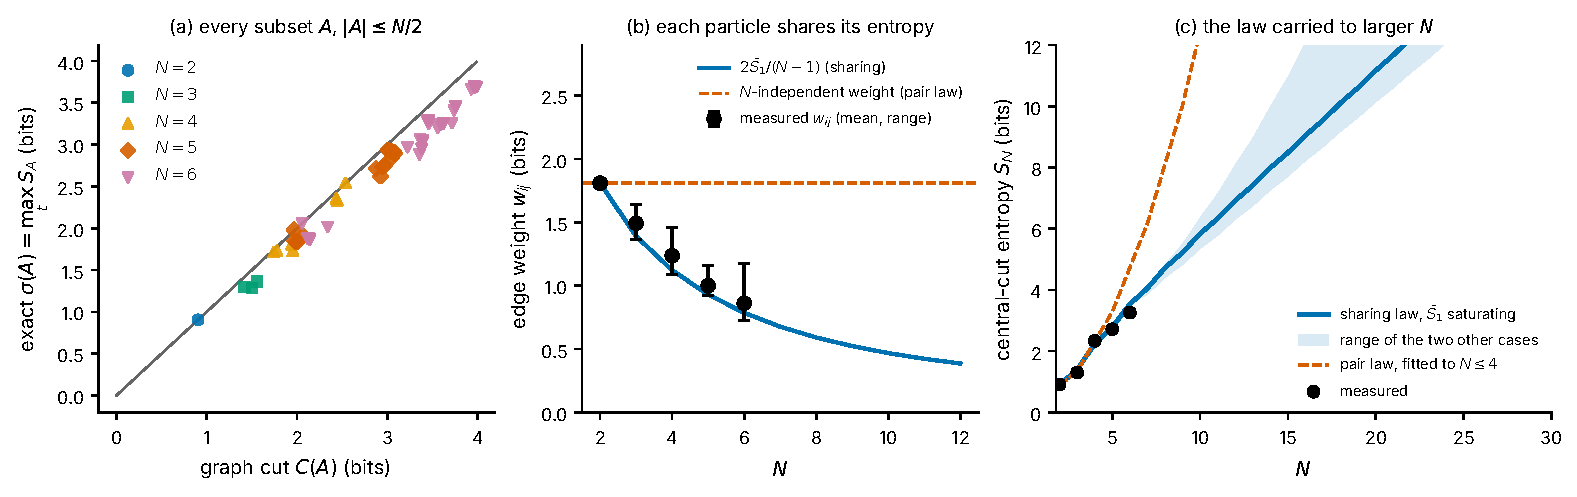
\includegraphics[width=\textwidth]{figures/fig_entropy.pdf}
\caption{\textbf{The graph explains the entropy, and why its growth falls.} (a) Exact $\sigma(A)=\max_tS_A$ against the graph cut $C(A)$ for every subset with $|A|\le N/2$ at $N\le6$. (b) Mean edge weight $w_{ij}$ with its range, against the sharing
law $2\bar S_1/(N-1)$ and against the $N$-independent weight that the pair-counting law assumes. (c) Central-cut entropy against $N$: measured (black), the pair law fitted to $N\le4$ (dashed), and the sharing law carried to larger $N$ (Section~\ref{sec:larger}); shading spans the other two
scenarios for the one-particle entropy. Computed from the stored time series of each run (Appendix~\ref{app:numerics}).}
\label{fig:entropy}
\end{figure}

\paragraph{Test.} The graph reproduces the entropy of every subset at $N\le6$ (Fig.~\ref{fig:entropy}a): it overestimates the exact entropy by up to $\num{graph_maxdev}$ bit ($N=6$) and underestimates it by at most $\num{graph_maxunder}$ bit. The overcount at $N=3$ is a property of the time maxima: at fixed $t$ the graph is exact there, but the maximum over $t$ of each edge occurs at different times. The graph is also a good guide to the layout: the order that minimizes the maximal prefix cut on the graph costs at most a few hundredths of a bit more than the exact optimum, and the rank correlation between graph and exact costs is high at $N=3,6$ and modest at $N=4,5$ (Table~\ref{tab:measured}). It finds a near-best order but ranks the rest unreliably there.

\paragraph{Why the growth falls: each particle shares a finite entropy (a description, not a derivation).}
The measured edge weights are nearly uniform within each $N$ and fall with $N$ (Fig.~\ref{fig:entropy}b, Table~\ref{tab:measured}). In a pure state a particle's entropy is the mutual information it shares with all the others, $\sum_jI_{ij}\approx2S_i$; the measured ratio is between $\num{mono_lo}$ and $\num{mono_hi}$ for all $N$ and $i$. The sum rule is an identity only when monogamy holds, and a finite entropy does not by itself force equal weights (a state can concentrate it on a few partners); we use the near-equality as an observation. In words: each particle has a finite amount of entanglement to give, and the more partners there are, the thinner each share. If each particle spreads its entropy evenly over its $N-1$ partners,
\begin{equation}
w_{ij}\simeq\frac{2\bar S_1}{N-1},\qquad
S_N\simeq C(\{1..b\})=\frac{b(N-b)}{N-1}\,\bar S_1(N),\quad b=\lfloor N/2\rfloor,
\label{eq:sharing}
\end{equation}
where $\bar S_1$ is the mean one-particle entropy and the prefactor is $\simeq(N+1)/4$. The law reproduces the measured weights and central cuts; at $N=5,6$ the cut it gives lies inside the layout bracket, as a size-class average should (Lemma~\ref{lem:chord}), and above the natural-order cut. The pair-counting law is the opposite assumption, an $N$-independent weight on each of the $\lfloor N/2\rfloor\lceil N/2\rceil$ crossing pairs. A particle cannot give every one of a growing number of partners the same entropy, and the data show it does not: fitted to $N\le4$ the pair law overshoots at $N=5$ and $N=6$ by more than the spread of layouts and lies above even the worst layout, and the linear law fitted the same way is high by an amount comparable to that spread (Table~\ref{tab:measured}, Table~\ref{tab:scen}).

\paragraph{Why the shares thin out.} The saturation of $\bar S_1$ and the $1/(N-1)$ fall of the shares are what a monogamy relation for mutual information describes: if one particle has a bounded entanglement capacity, the share it gives to each partner must fall as the number of partners grows~\cite{hayden2013}. The measured sum rule sits at the boundary of that relation, where the sharing law is exact, and a similar dilution of orbital mutual information among many partners is seen in correlation graphs of molecules~\cite{rissler2006,barcza2011}. Monogamy of mutual information is not a general property (above), so this is a consistency argument, not a derivation. With the shares thin, the central cut grows as $b(N-b)/(N-1)\simeq N/4$ times $\bar S_1$, that is linearly in $N$ once $\bar S_1$ has saturated, and not as the $b(N-b)\sim N^2/4$ of the pair-counting law. This is the growth that decides the cost of a matrix-product state, whose bond dimension is bounded below by the exponential of the cut entropy~\cite{schuch2008}. What the data support is the rejection of the pair law at $N=6$; they do not yet separate the sharing law from other linear growth.

\begin{figure}[t]
\centering
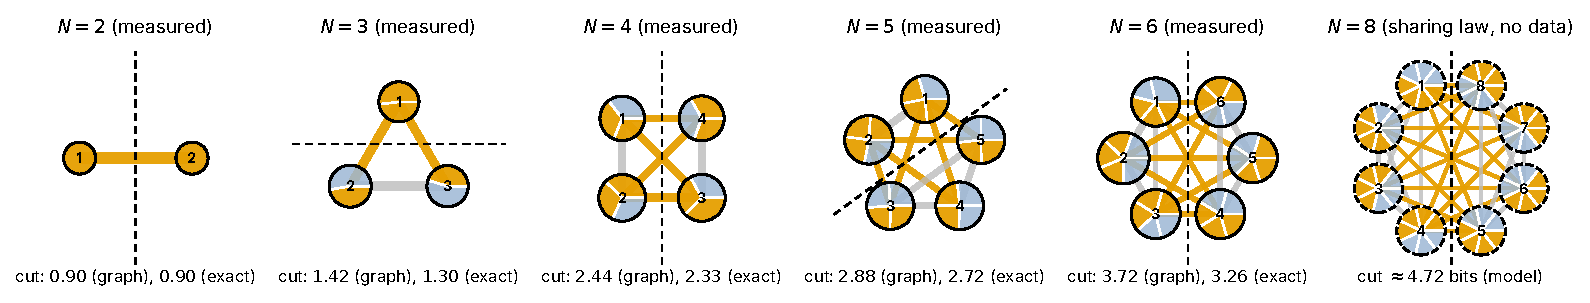
\includegraphics[width=\textwidth]{figures/fig_venn.pdf}
\caption{\textbf{Adding particles to the correlation graph.} Each disk is a particle; its area is the entropy it shares, $\sum_jw_{ij}/2$, on the same scale in every panel. A disk is divided into one petal per partner (angle proportional to $w_{ij}$),
and the petals of $i$ and $j$ are joined by a ribbon of width proportional to $w_{ij}$. The dashed line is the central cut: orange ribbons cross it, and the entropy across the cut is their total width ($C$ in the caption of each panel; exact value for comparison). Adding a particle
adds a disk and $N$ ribbons, but the old disks cannot grow much, so every petal, and every ribbon, thins; the number of crossing ribbons grows as $b(N-b)$. The panel at $N=8$ is drawn from the sharing law, not from data (dashed outlines).}
\label{fig:venn}
\end{figure}

Fig.~\ref{fig:venn} draws this. Going from $N=2$ to $5$ the graph gains disks and ribbons that cross the cut, and each ribbon becomes thinner; the net growth of the cut is the product of the two.


\paragraph{What is not established.}
\begin{itemize}[itemsep=0.15em]
\item Eq.~\eqref{eq:Cgraph} is validated on $N\le6$ only. It is an estimator and a layout heuristic, not a bound, and with time-maximal weights it overcounts.
\item Eq.~\eqref{eq:sharing} assumes that each particle shares its entropy evenly with its partners and that the graph stays dense; the data are consistent with the first, and the second may fail for large, spatially extended clusters.
\item The graph cannot say whether $\bar S_1$ saturates beyond $N=6$. That is the one input of the extrapolation below.
\end{itemize}


\subsection{\texorpdfstring{Carried to larger $N$}{Carried to larger N}}
\label{sec:larger}

Eq.~\eqref{eq:sharing} turns the question ``how does $\SN$ grow?'' into ``how does $\bar S_1(N)$ behave?''. The one-particle entropy is bounded (by $\log_2k$ at fixed $k$) and its measured increments shrink from $N=3$ on (Table~\ref{tab:measured}). We carry it forward in three stated scenarios, none of which is a measurement beyond $N=\num{Nmax_measured}$ (parameters and extrapolated values in Table~\ref{tab:scen}):
\begin{itemize}[itemsep=0.15em]
\item \emph{saturating (fit):} $\bar S_1(N)=S_\infty-(S_\infty-\bar S_1(2))e^{-(N-2)/\tau}$ with two parameters fitted to the measured values and anchored at $N=2$;
\item \emph{saturated at $N=\num{Nmax_measured}$:} $\bar S_1$ stays at its last measured value, the earliest saturation the data allow (the optimistic case for the classical side);
\item \emph{keeps growing:} $\bar S_1$ grows by the mean of the last two measured increments per particle (the pessimistic case for the classical side; the central cut then grows as $N^2$).
\end{itemize}
In the first two cases $\SN$ is asymptotically linear with slope $\bar S_1^\infty/4$ per added particle. Fig.~\ref{fig:entropy}c shows the three curves against the pair law.

\begin{table}[ht]
\centering
\small
\caption{The three scenarios for the one-particle entropy $\bar S_1(N)$ beyond the simulated sizes, the growth laws fitted to smaller $N$, and what they predicted for the central bond (bits). The sharing-law rows were fitted to $N\le5$ and give the central cut they predicted at $N=6$ before that run, and its excess over the measured $S_6=\num{S6_cen}$; the pair-counting and linear laws were fitted to $N\le4$. \emph{Slope}: asymptotic growth per added particle (the sharing law with saturating $\bar S_1$ is linear in $N$; with growing $\bar S_1$ it grows as $N^2$). The last three columns are the extrapolated central bond. None of these is a measurement beyond $N=\num{Nmax_measured}$.}
\label{tab:scen}
\begin{tabular}{llcccccc}
\toprule
scenario & parameters & slope & $N=6$ & excess & $N=8$ & $N=12$ & $N=16$ \\
\midrule
sharing, $\bar S_1$ saturating (fit) & $S_\infty=\num{fit_Sinf}$, $\tau=\num{fit_tau}$ & 0.53 & 3.71 & 0.46 & 4.72 & 6.92 & 9.05 \\
sharing, $\bar S_1$ saturated at $N=6$ & $\bar S_1=\num{S1_last}$ & 0.48 & 3.39 & 0.13 & 4.41 & 6.31 & 8.22 \\
sharing, $\bar S_1$ keeps growing & $+\num{inc_pess}$ per particle & $\propto N^2$ & 3.90 & 0.64 & 4.82 & 8.08 & 12.07 \\
pair-counting law & fit to $N\le4$ & $\propto N^2$ & 4.73 & 1.47 & 8.11 & 17.76 & 31.27 \\
linear law & fit to $N\le4$ & 0.71 & 3.66 & 0.40 & 5.09 & 7.95 & 10.81 \\
\bottomrule
\end{tabular}
\end{table}



\paragraph{The $N=6$ comparison.} The sharing law fitted to $N\le5$ and the pair and linear laws fitted to $N\le4$ give predictions for the central bond at $N=6$ (Table~\ref{tab:scen}), which the simulation at $N=6$ ($S_6=\num{S6_cen}$ bit, $k=12$) tests. It decides against the pair law, which is too high and above even the worst layout. It does not vindicate the sharing law as a predictor: all three scenarios overshoot, and so does the linear law. The assumption behind the scenarios holds, since the one-particle entropy grows by very little, and the sharing law fed with the measured $\bar S_1$ gives a value inside the layout bracket (Table~\ref{tab:measured}). What it overstates is the prefactor: the natural-order bond lies below the size-class average, as it does, by less, at $N=5$. The curves of the three scenarios are refitted through the $N=6$ point, so the walls of Section~\ref{sec:walls} use $N\le6$. One further point cannot separate the sharing law from linear growth: the measured step is close to the asymptotic slope of the sharing law.

The prefactor can also be tested on the stored runs. Fed with each run's own $\bar S_1$, the sharing law reproduces the measured central entropy of all correlated-start runs ($N=2$--$\num{shr_Nmax}$, every stored $k$) to within a measured-to-law ratio of $\num{shr_lo}$--$\num{shr_hi}$, so the small overshoot is a property of the correlated start across $N$ and $k$, not of one run. The product start, a quench, does not follow the law at $N=4$, $k=12$ (ratio $\num{shr_prod_N4}$); at $N=3$ it still holds, with a much larger $\bar S_1$.

\FloatBarrier

\section{What the prepared state is made of}
\label{sec:static}

Section~\ref{sec:measured} measured how much entanglement the evolved state carries. What that entanglement means, and what the task costs, depends on a different question: \emph{what is the start state in terms of the eigenstates of $\hat H$?} If it lies on very few of them, the signal $\langle\Op\rangle(t)$ is a short sum of cosines whose frequencies, weights and amplitudes are static quantities of $\hat H$. This section reports the low levels of $\hat H$ at the resonance tilt and the weight of the correlated start on each (no propagation) for $N\le5$, and for $N=6$ in one basis; Table~\ref{tab:static} summarizes it and Table~\ref{tab:start} (Appendix~\ref{app:static}) has every case. The \emph{pair} is the two levels of largest weight, at energies $E_a<E_b$, with $J=(E_b-E_a)/2$ and total weight $B_2$.

\paragraph{What is observed.}
\begin{itemize}[itemsep=0.15em]
\item The start is two eigenstates, the cluster before and after one particle has moved, plus a dressing by soft internal levels whose weight grows with $N$.
\item An exact reflection symmetry removes all other levels from the picture, and the transfer of more than one particle lies far from the pair.
\item Most of the cut entropy of Section~\ref{sec:measured} is present without any tunneling.
\item The number of cosines the signal needs grows with $N$; the tunneling regime itself ends near $N\approx\num{fu_Ntop_lo}$--\num{fu_Ntop_hi} at fixed trap depth.
\end{itemize}

\begin{table}[ht]
\centering
\footnotesize
\caption{What the prepared state is made of (Section~\ref{sec:static}; every case is in Table~\ref{tab:start}). Correlated start at the resonance tilt $c^*$, $k=20$ modes per particle unless stated. \emph{Pair}: splitting $2J$ and weight $B_2$ of the two levels of largest weight, and $B_2$ at the largest basis computed (with that $k$). \emph{Outside the pair}: weight within $J$, at $1$--$3J$ and beyond $3J$ of the nearer level of the pair. \emph{Signal}: number of cosines of a free fit that brings the residual to $10\%$ and to $5\%$ of the standard deviation of $\langle\Op\rangle(t)$ (largest basis stored; the $N=6$ fit did not reach $5\%$ with eight, $k=12$, not converged).}
\label{tab:static}
\begin{tabular}{rcccccccccc}
\toprule
 & & \multicolumn{3}{c}{pair} & \multicolumn{3}{c}{outside the pair} & \multicolumn{2}{c}{cosines for} \\ \cmidrule(lr){3-5}\cmidrule(lr){6-8}\cmidrule(lr){9-10}
$N$ & $c^*$ & $2J$ & $B_2$ & $B_2$ at largest $k$ & $<J$ & $1$--$3J$ & $\ge3J$ & $10\%$ & $5\%$ \\
\midrule
2 & 0.70 & 0.192 & 0.978 & 0.978 ($k=20$) & 0.000 & 0.010 & 0.013 & 1 & 3 \\
3 & 1.31 & 0.193 & 0.955 & 0.955 ($k=20$) & 0.000 & 0.017 & 0.028 & 2 & 3 \\
4 & 2.02 & 0.218 & 0.906 & 0.934 ($k=32$) & 0.000 & 0.056 & 0.024 & 3 & 5 \\
5 & 2.62 & 0.233 & 0.812 & 0.836 ($k=24$) & 0.007 & 0.114 & 0.010 & 4 & 8 \\
6 ($k=12$) & 3.66 & 0.437 & 0.729 & -- & 0.194 & 0.013 & 0.000 & \ensuremath{>}8 & \ensuremath{>}8 \\
\bottomrule
\end{tabular}
\end{table}


\subsection{Two levels plus a dressing}
\label{sec:twolevel}

\begin{figure}[ht]
\centering
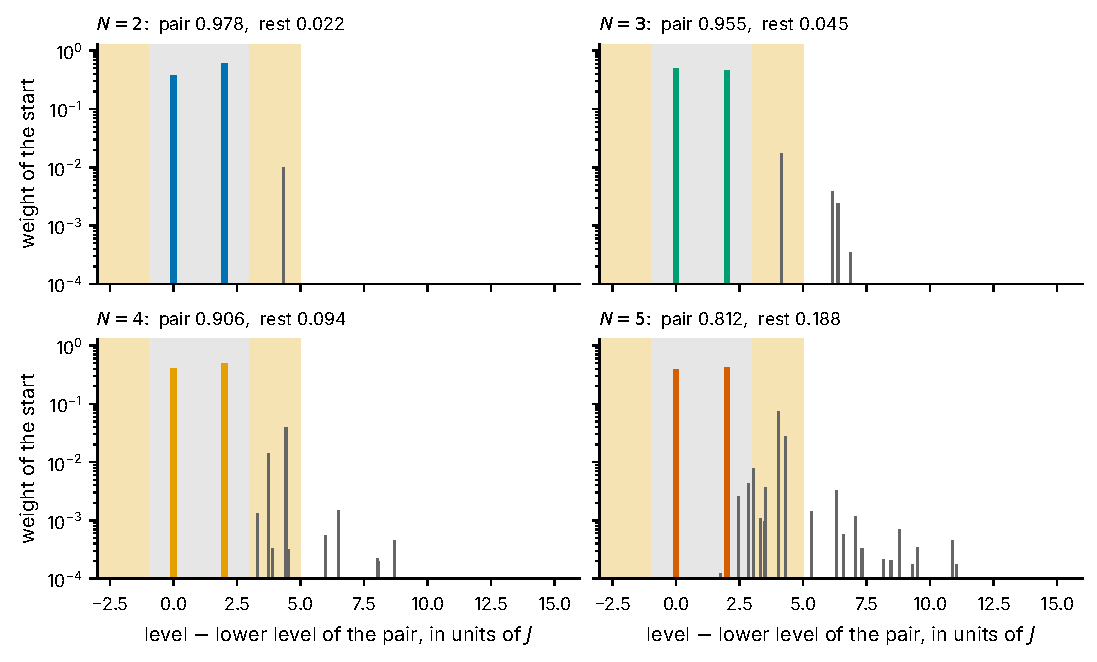
\includegraphics[width=0.8\textwidth]{figures/fig_spectrum.pdf}
\caption{\textbf{The correlated start in the eigenbasis of $\hat H$} at the resonance tilt, $k=20$ modes per particle. Each line is one eigenlevel; its height is the weight of the start on it, on a logarithmic axis; the horizontal axis is the distance from the lower level of the pair in units of $J$. Colour: the pair. Shading: within $J$ of either level of the pair (grey) and $1$--$3J$ from it (orange). The title of each panel gives the weight of the pair and of the rest; at $N=4,5$ part of the rest sits on levels not computed (Fig.~\ref{fig:dressing}b).}
\label{fig:spectrum}
\end{figure}

Table~\ref{tab:static} and Fig.~\ref{fig:spectrum} show that for $N=2,\dots,5$ the start lies on two eigenstates and a thin cloud of others: the symmetric and antisymmetric combinations of the all-left cluster (all particles in the crowded valley) and of the cluster with particle $0$ moved to the other valley. Their splitting $2J$ is the frequency of the main oscillation. The weight of the pair falls with $N$ at fixed basis size and rises with $k$ (Fig.~\ref{fig:dressing}a); it converges at $N=4$ but not at $N=5$, and no $N=6$ spectrum is converged. The small-basis values at $N=4$ ($k=12$) are a basis artefact.

\begin{figure}[ht]
\centering
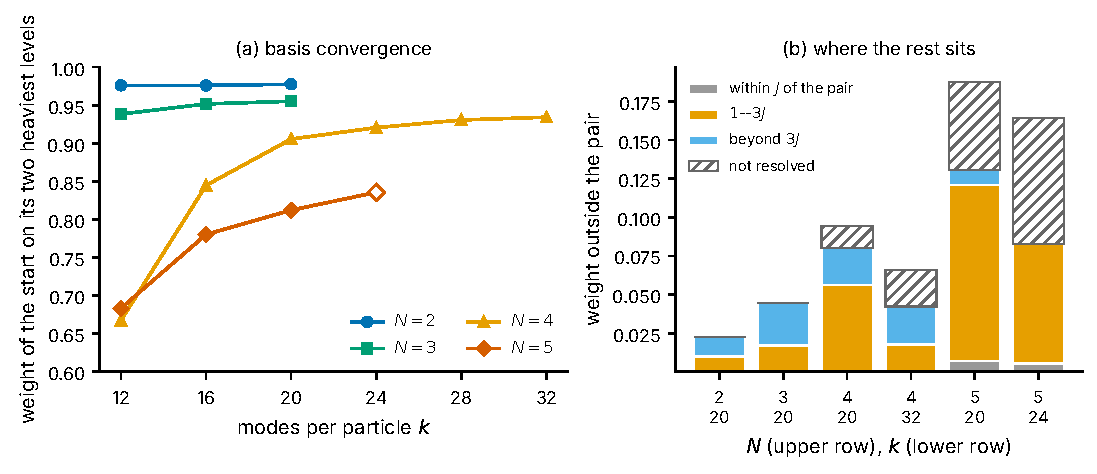
\includegraphics[width=0.8\textwidth]{figures/fig_dressing.pdf}
\caption{\textbf{The pair and the dressing.} (a) Weight of the start on the pair against the number of modes per particle $k$ (lines, $N=2$--$5$). The open symbol is a Lanczos list that resolves only part of the weight (Table~\ref{tab:start}). The $N=4$ curve converges; the $N=5$ curve has not. (b) The weight outside the pair, split by the distance to the nearer level of the pair: within $J$ (grey), $1$--$3J$ (orange), beyond $3J$ (blue), and weight not on any computed level (hatched). Upper axis label: $N$; lower: $k$. At $k=12$ a large part of the rest sits within $J$ of the pair at $N=4,5$; that part is a basis artefact (it vanishes for $k\ge16$) and is not shown.}
\label{fig:dressing}
\end{figure}

The weight outside the pair (Fig.~\ref{fig:dressing}b) is small far from the pair and about the same for all $N$; the part that grows with $N$ sits at $1$--$3J$, on internal levels softer than the transfer itself. This is the dressing of the transfer by soft internal motion of the cluster, and it is the quantity on which the scaling of the problem depends (Section~\ref{sec:openproblem}). It does not fall when the barrier is raised, although $J$ does (Table~\ref{tab:Ascan}).

\subsection{One transfer channel and an exact symmetry}
\label{sec:parity}

The pair is a closed two-state system at $N\le4$ for three structural reasons (Fig.~\ref{fig:parity} and Table~\ref{tab:levels}, Appendix~\ref{app:static}). The reflection $y_i\to-y_i$ of all particles is an exact symmetry of $\hat H$ and $\Op$; the start is even, so the odd levels, including those between the two members of the pair, carry no weight. The transfer of more than one particle is far from the pair (\emph{sector exclusion}). And because particles are distinguishable, the states in which another particle moves instead of particle $0$ lie a few $J$ from the pair (\emph{label fragmentation}); that margin is why the offsets $C_0$ matter (Appendix~\ref{app:choice}), it is not large, and it is not known to survive for $N\gtrsim6$.

\subsection{Most of the entropy is static}
\label{sec:static-entropy}

\begin{figure}[htpb]
\centering
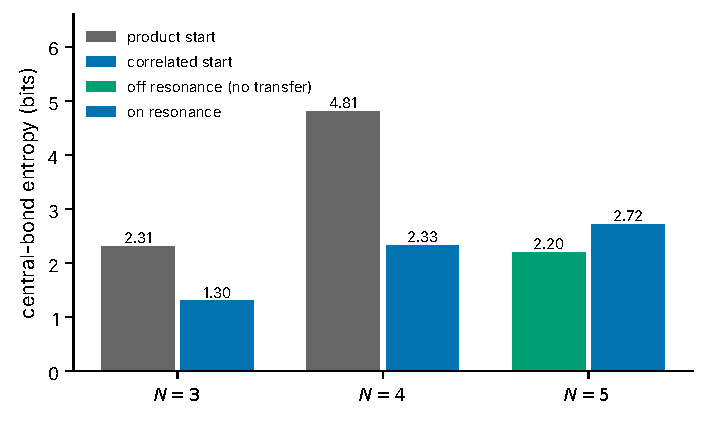
\includegraphics[width=0.5\textwidth]{figures/fig_control.pdf}
\caption{\textbf{How much of the central-bond entropy is already there before anything moves.} Left and middle: the product start (a quench that ignores the correlation hole of particles sharing a valley) against the correlated start. Right, $N=5$: the same start off resonance, where the cluster stays in one isomer, against the resonant run. The off-resonance entropy is $\num{off_diff}$ bit below the resonant one.}
\label{fig:control}
\end{figure}

Away from resonance the cluster stays in one isomer and no tunneling takes place, yet the central-bond entropy keeps most of its resonant value (Table~\ref{tab:control}, Fig.~\ref{fig:control}). Together with the closed two-state structure this changes the reading of Section~\ref{sec:measured}: those entropies are, for the most part, the static entanglement of the correlated isomers, namely the correlation hole of particles that share a valley, which the correlated start carries from $t=0$. In the ideal case in which the start is exactly a superposition $a|F\rangle+\sum_ib_i|I_i\rangle$ of a product state $|F\rangle$ and states with one particle moved, every cut has Schmidt rank at most two, so the entropy added by the transfer is at most one bit for any $N$ (Proposition~\ref{prop:cond}). Matrix-product-state cost curves built on the entropy of the evolved state price the isomers; they do not by themselves show that the dynamics is hard.

\begin{table}[ht]
\centering
\small
\caption{The control without tunneling: $N=5$, $k=12$, correlated start, away from resonance ($c=\num{off_c}$, the start stays in one isomer) against the resonant run (Fig.~\ref{fig:control}). Same window $T=\num{off_T}$\num{off_lb}.\num{off_note}}
\label{tab:control}
\begin{tabular}{lrr}
\toprule
 & off resonance & resonance \\
\midrule
lowest value of $\langle\Op\rangle/\langle\Op\rangle(0)$ & 0.75 & 0.27 \\
central bond $\Snat$ & 2.20 & 2.72 \\
mean one-particle entropy $\bar S_1$ & 1.60 & 1.88 \\
edge weights $w_{ij}$ (range) & 0.44--1.15 & 0.92--1.16 \\
largest graph excess over the exact entropy & 0.30 & 0.48$^\dagger$ \\
rank correlation, graph against exact orders & 0.87 & 0.46 \\
time of the central-bond maximum & 144 & 197 \\
\bottomrule
\end{tabular}
\par\smallskip\footnotesize $^\dagger$ largest over all $N\le6$ (Fig.~\ref{fig:entropy}a), not for $N=5$ alone.
\end{table}


\subsection{A conditional reduction and the number of cosines}
\label{sec:cond}

\begin{cprop}\label{prop:cond}\stC{}
Let $|F\rangle$ be the correlated all-left state and $|I_0\rangle$ the correlated state with particle $0$ on the right. Suppose that for $0\le t\le\Tobs$ the evolved state stays, up to an amplitude error $\delta$, in the span $\mathcal S$ of $|F\rangle$, $|I_0\rangle$ and $M$ further eigenstates $|s_1\rangle,\dots,|s_M\rangle$ of $\hat H$ (the sidebands). Then
\[
f(t)=\sum_{m,n}c_m^\ast c_n\,O_{mn}\,e^{i(E_m-E_n)t}+O(N\delta),\qquad m,n\in\{1,\dots,M+2\},
\]
is a sum of at most $(M+2)(M+3)/2$ cosines whose frequencies, weights and amplitudes are static quantities of $\hat H$. In the ideal case $M=0$, with product states of left and right orbitals and any number of labelled states with at most one particle on the right, every particle cut has Schmidt rank at most two and entropy at most one bit for any $N$. For correlated states of bond dimension at most $\chi_0$ in a common ordering, the bond dimension of the state is at most $(M+2)\chi_0$ at all times.
\end{cprop}

The first statement is a finite-dimensional superposition, and the rank bounds follow because $a|F\rangle+\sum_ib_i|I_i\rangle$ is a sum of two product vectors across any cut (proof in Appendix~\ref{app:proofs}). What is not elementary is whether $M$ stays small and whether the static inputs are cheap.

\begin{figure}[htpb]
\centering
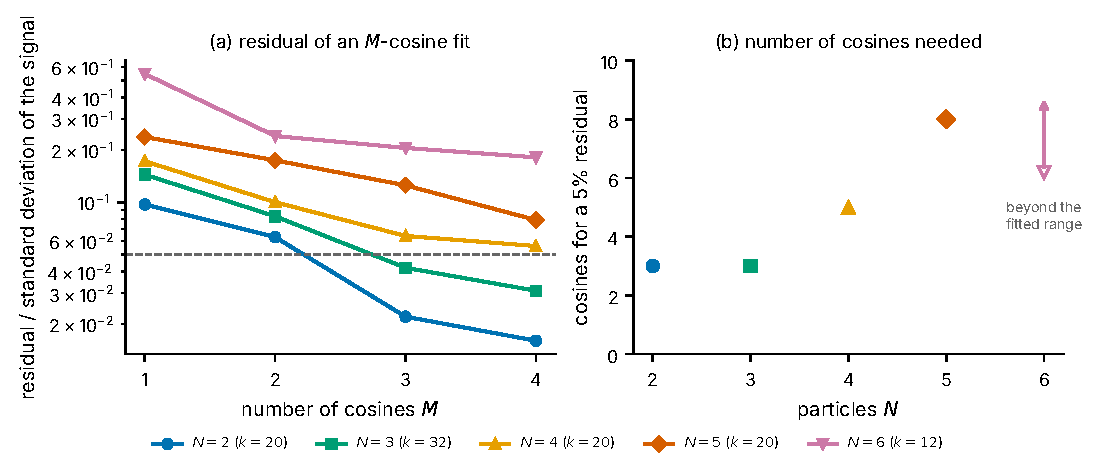
\includegraphics[width=0.8\textwidth]{figures/fig_cosines.pdf}
\caption{\textbf{How many cosines the signal needs.} (a) Residual of a free fit of $M$ cosines to $\langle\Op\rangle(t)$ on the stored time series ($T=\num{Tprot}$), in units of the standard deviation of the signal, for the largest basis size available at each $N$. (b) The number of cosines for a residual of $5\%$; the open symbol at $N=6$ marks that no fit with up to eight cosines reached it (one run, $k=12$, not converged). The fit chooses its frequencies freely; it is a measure of the structure of the signal, not a prediction from static energies.}
\label{fig:cosines}
\end{figure}

A few cosines do explain the signal at $N=2,3$, but the number needed for a given residual grows with $N$ (Table~\ref{tab:mc}, Table~\ref{tab:static}, Fig.~\ref{fig:cosines}b), the same trend as the dressing seen in the time domain. This cannot say whether the growth continues, and it does not by itself decide the cost of the task, since obtaining $M$ frequencies and weights is a static problem.

\subsection{Where the regime ends}
\label{sec:regimeend}

\begin{figure}[htpb]
\centering
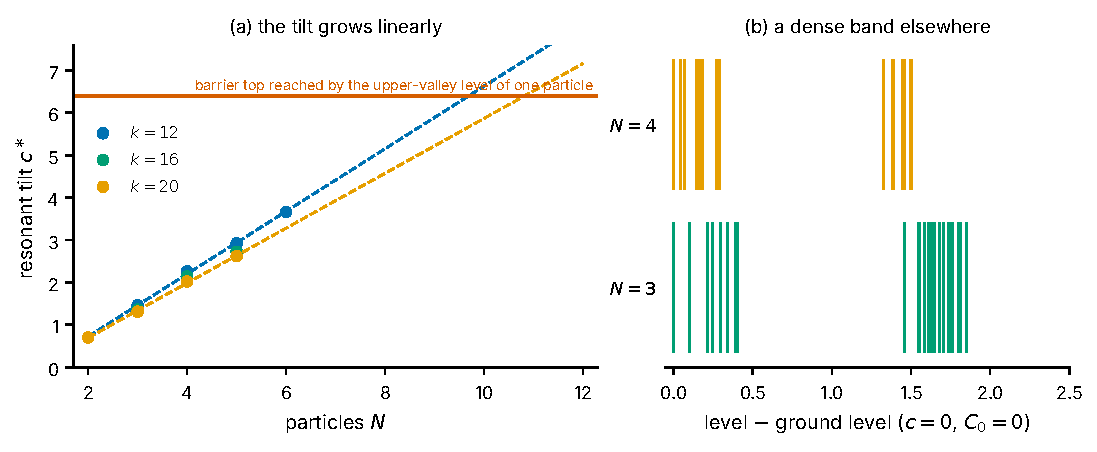
\includegraphics[width=0.8\textwidth]{figures/fig_tilt.pdf}
\caption{\textbf{The resonance tilt and the end of the regime.} (a) The tilt $c^\ast$ at which the all-left and one-moved clusters are degenerate, against $N$, for three basis sizes; it rises by about $\num{fu_cstep_lo_k12}$--$\num{fu_cstep_hi_k12}$ per particle at $k=12$, nearly linearly. Dashed lines extend the straight lines through the measured points. The horizontal line is the tilt at which the lowest level localized in the raised valley of the one-particle tilted well reaches the top of the barrier ($c=\num{fu_ctop}$; finite differences, a rough one-body picture). (b) With a symmetric trap and no tilt or offsets ($c=0$, $C_0=0$) the lowest levels form a dense band with a gap above it: a different task from the tilted transfer.}
\label{fig:tilt}
\end{figure}

The resonant tilt rises nearly linearly with $N$ and shows no bending through the measured sizes (Fig.~\ref{fig:tilt}a). In the one-particle picture of the tilted well the upper-valley level reaches the top of the barrier at a tilt that the straight lines reach at $N\approx\num{fu_Ntop_lo}$--\num{fu_Ntop_hi}. The entropy extrapolations of Section~\ref{sec:larger} cross this point, and whether the transfer continues as a many-body process past it is open. A trap depth that grows with $N$ is a different family: the rule must be fixed in advance, and the classical and quantum costs recomputed. With a symmetric trap and no tilt (Fig.~\ref{fig:tilt}b) the lowest band is a dense many-occupation manifold with permutation multiplets, a different task that was not simulated in time.

\subsection{The open problem}
\label{sec:openproblem}

The cost of the task, as defined, is the cost of the static \emph{dressed-transfer spectrum}: the number $M(N)$ of sidebands needed for error $\varepsilon N$, and the cost of their energies, weights and matrix elements. If the dressing is harmonic (a displaced, Duschinsky-mixed oscillator bath) the problem is a spin--boson problem, which is heuristically easy classically. If it is strongly anharmonic with soft modes comparable to $J$, no classical method with a known polynomial cost applies. Sign-free structure (distinguishable particles) makes imaginary-time and instanton methods applicable (Section~\ref{sec:mc}), but neither a polynomial bound nor a hardness proof is known. The measurements say only that the weight outside the pair grows with $N$ at fixed basis size, that the growing part sits at $1$--$3J$, and that $J$ is not small compared with it at $N=4,5$.

\paragraph{Hardness is unprovable for this fixed family.} The observable is a function of positions, so its time derivative is bounded by a constant times $N$ and $f$ can be tabulated to the allowed error on a finite set of points for every $N$ (Appendix~\ref{app:static}). The table exists but is not an algorithm (a non-uniform statement), so no reduction-based hardness result is possible for the task as defined. Statements can only concern the scaling of the best known methods, or a different family with free instance parameters.

\paragraph{What is not established.}
\begin{itemize}[itemsep=0.15em]
\item The dressing series has few points at basis sizes that are still moving at $N=5$ (Table~\ref{tab:start}); extrapolating it to $N=6,7$ is not a measurement.
\item Gaussianity of the dressing is undecided: the test is the harmonic (Huang--Rhys) prediction of $B_2$ from the two constrained isomers against the measured $B_2$ at $k\ge16$, and it was not run.
\item $N=6$ and the basis convergence at $N=5$ are unfinished; everything in this section is for $N\le5$ unless stated.
\item The cosine counts are free fits to one stored signal per case, not predictions.
\item No claim is made that a classical method reproduces the signal at large $N$, nor that none does.
\end{itemize}

\FloatBarrier

\section{Discussion}
\label{sec:discussion}

This section sets the measurements against the costs. Subsection~\ref{sec:walls} says where the classical routes stop, Subsection~\ref{sec:quantum} what a quantum computer would pay and what window the two bounds draw, and Subsection~\ref{sec:open} what the report does and does not establish and what is open.

\subsection{Where the classical routes stop}
\label{sec:walls}

Evaluating the inequalities of Section~\ref{sec:framework} for the budgets of Table~\ref{tab:params} gives the first failing $N$ of each route (Table~\ref{tab:walls}). Full-state storage fails by a count, early on the grid and later in a compressed basis. The tensor-network wall is Eq.~\eqref{eq:Nstar} evaluated on the entropy of Section~\ref{sec:larger}: under the three scenarios for the one-particle entropy it lies on the grid between $N=\num{wall_pess_grid}$ (entropy keeps growing) and $N=\num{wall_opt_grid}$ (saturated at its $N=\num{Nmax_measured}$ value) \stC{}, with the compute budget binding first (Fig.~\ref{fig:walls}). Since most of that entanglement is static (Section~\ref{sec:static}), the wall prices the representation of the evolved state, not the task.

\begin{table}[ht]
\centering
\footnotesize
\caption{Where each classical route first fails (first failing $N$) for the budgets of Table~\ref{tab:params}. Exact diagonalization is an exact count; the tensor-network rows evaluate the cost model of Prop.~\ref{prop:tn} on the graph law of Section~\ref{sec:larger} under three assumptions about the one-particle entropy beyond the largest simulated $N$. In parentheses: the same with the numerical Schmidt rank $\chi(10^{-3})$ charged instead of $2^{S}$, at the ratio measured at $N=6$ ($+\num{chi_shift}$ bits).}
\label{tab:walls}
\begin{tabular}{L{4.0cm}L{5.3cm}cc}
\toprule
Route & Assumption & grid, $d=\num{d_grid}$ & modes, $d=\num{d_mode}$ \\
\midrule
Exact diagonalization, distinguishable & exact count & 4 & 8 \\
Exact diagonalization, bosonic & exact count & 4 & 17 \\
\midrule
Tensor networks & entropy keeps growing at the $N=4\to6$ rate & 13 (7) & 18 (13) \\
Tensor networks & one-particle entropy saturates (fit) & 15 (7) & 25 (16) \\
Tensor networks & one-particle entropy saturated at $N=6$ & 16 (7) & 27 (17) \\
\bottomrule
\end{tabular}
\end{table}


\begin{figure}[t]
\centering
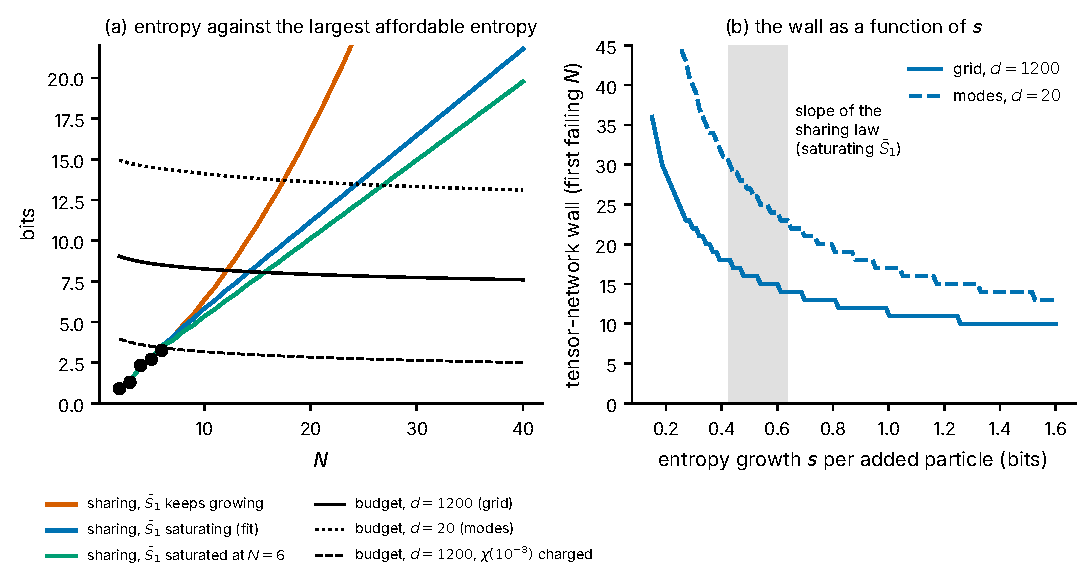
\includegraphics[width=\textwidth]{figures/fig_walls.pdf}
\caption{\textbf{The tensor-network wall.} (a) The central-cut entropy under the three scenarios of Section~\ref{sec:larger} against the largest entropy that the memory and compute budgets of Table~\ref{tab:params} allow (grid and mode basis;
dashed: grid budget when the numerical Schmidt rank $\chi(10^{-3})$ is charged instead of $2^{S}$, Section~\ref{sec:seed}). The wall is the first crossing. (b) The wall for a constant growth $s$ per added particle anchored at the last simulated $N$ (Eq.~\eqref{eq:Nflop}); the grey band is the asymptotic slope
of the sharing law. Computed from the measured entropies and the budgets of Table~\ref{tab:params}.}
\label{fig:walls}
\end{figure}

A matrix-product state was also run (density-matrix-renormalization-group start, two-site time-dependent variational evolution) as an independent check of the counting model. It reproduces the exact entropies to a few hundredths of a bit or better (Table~\ref{tab:mps}, Fig.~\ref{fig:tn}a) but is slower than the exact code at the sizes tried, so it reaches only $N\le5$ and extends no data. Two corrections to the model go in opposite directions, and neither is converged. The numerical Schmidt rank $\chi(10^{-3})$ exceeds $2^{S}$ by a factor that grows with $N$ and $k$ (Fig.~\ref{fig:tn}b); charging it at the ratio measured at $N=6$ adds $\num{chi_shift}$ bits and moves the grid wall to the values in parentheses in Table~\ref{tab:walls}. Charging the central bond on every bond, and the natural order instead of a better tree, overstates the cost (Lemma~\ref{lem:chord}). The wall moves by only $\log_2f/(3s)$ particles for a factor $f$ in the budget (Eq.~\eqref{eq:Nflop}), so the lower edge of the window is the soft quantity of the bounds, and Fig.~\ref{fig:regime} shades it rather than cutting it. The measured cost per step is nearly flat in $\chi$ at these sizes (Fig.~\ref{fig:tn}c), so the model's prefactor is a lower bound and has not been tested where the bond cap matters.

\begin{table}[ht]
\centering
\small
\caption{A matrix-product state (density-matrix-renormalization-group start, two-site time-dependent variational evolution) against the exact propagation of the same case, correlated start, resonant tilt, window $T$ (shorter than $T=\num{Tprot}$ so that the exact run is cheap). $S_{\rm cen}$: central-bond entropy (bits); $\max\Delta S$: largest difference over every cut both methods measured and every snapshot; $\chi_{10^{-3}}$: numerical Schmidt rank of the central bond (at odd $N$, of the two central bonds the one with the larger entropy); $\chi_{\max}$: cap on the bond dimension (binding where $\chi_{10^{-6}}$ of the MPS equals it). Last column: wall time of the MPS over that of the exact code (a shared four-core machine; an order of magnitude only). The $k=6$ rows validate the method in a saturated basis; the $k=12$ row is capped at $\chi_{\max}$ and its $S_{\rm cen}$ is $\num{tn_k12_dSc}$ bit below the exact value.}
\label{tab:mps}
\begin{tabular}{rrrrrrrrr}
\toprule
$N$ & $k$ & $T$ & $\chi_{\max}$ & $S_{\rm cen}$ MPS & $S_{\rm cen}$ exact & $\max\Delta S$ & $\chi_{10^{-3}}$ MPS / exact & slower by \\
\midrule
3 & 6 & 60 & 120 & 1.7332 & 1.7332 & \ensuremath{1.8\times10^{-5}} & 5 / 5 & 43$\times$ \\
4 & 6 & 60 & 120 & 2.4444 & 2.4449 & \ensuremath{5.9\times10^{-4}} & 18 / 18 & 76$\times$ \\
5 & 6 & 40 & 100 & 3.9603 & 3.9602 & \ensuremath{1.8\times10^{-3}} & 32 / 32 & 74$\times$ \\
4 & 12 & 40 & 64 & 2.2431 & 2.2640 & \ensuremath{2.8\times10^{-2}} & 32 / 35 & 146$\times$ \\
\bottomrule
\end{tabular}
\end{table}


\begin{figure}[t]
\centering
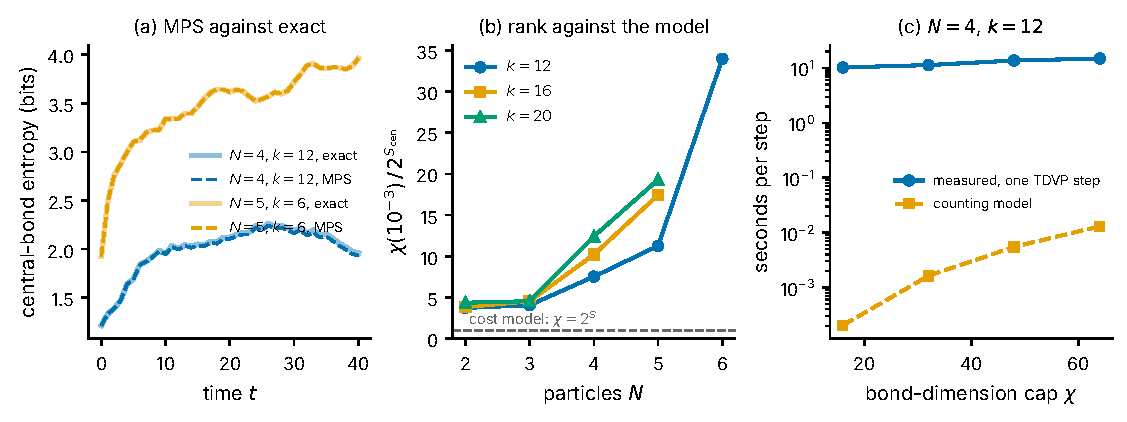
\includegraphics[width=\textwidth]{figures/fig_tn.pdf}
\caption{\textbf{What the matrix-product state measured.} (a) Central-bond entropy against time, matrix-product state (dashed) and exact (solid). (b) The numerical Schmidt rank $\chi(10^{-3})$ of the central bond in units of $2^{S_{\rm cen}}$, the value charged by the cost model, for the stored exact runs at $T=\num{Tprot}$. (c) Seconds per two-site step at $N=4$, $k=12$, measured, against the operation count of the counting model at the measured matrix-multiplication rate of the same machine.}
\label{fig:tn}
\end{figure}

By Eq.~\eqref{eq:scrit} the window at the simulated mass is non-empty if the growth per particle beyond $N=\num{Nmax_measured}$ exceeds $s_{\rm crit}$ (Table~\ref{tab:scrit}): existence is robust on the grid and marginal in the mode basis, and it refers to the entropy-based wall, which prices static entanglement, so it does not carry over to the dynamics.

\begin{table}[ht]
\centering
\small
\caption{Does a window exist at all? The growth per added particle $s_{\rm crit}$ (bits, Eq.~\eqref{eq:scrit}) that the central cut must exceed beyond $N=\num{Nmax_measured}$ for the window at the simulated mass to be non-empty with its upper end at $N_{\rm hi}$, against what the data give: the asymptotic slopes of the sharing law (saturated and saturating $\bar S_1$) and the last measured step.}
\label{tab:scrit}
\begin{tabular}{lccc}
\toprule
& $N_{\rm hi}=24$ & $N_{\rm hi}=40$ & $N_{\rm hi}=88$ \\
\midrule
$s_{\rm crit}$, grid & 0.25 & 0.13 & 0.05 \\
$s_{\rm crit}$, $20$-mode basis & 0.58 & 0.30 & 0.12 \\
\midrule
sharing-law slope, $\bar S_1$ saturated & \multicolumn{3}{c}{0.48} \\
sharing-law slope, $\bar S_1$ saturating (fit) & \multicolumn{3}{c}{0.53} \\
last measured step & \multicolumn{3}{c}{0.54} \\
\bottomrule
\end{tabular}
\end{table}


Imaginary-time Monte Carlo (Section~\ref{sec:mc}) is not excluded. Table~\ref{tab:mc} tests the picture it relies on: where the doublet test passes ($N=2,3$ and $N=4$, $k=20$) a prediction from the splitting alone is adequate; elsewhere the signal has several frequencies, and a prediction would need a handful of levels and weights, not one splitting.

\begin{table}[ht]
\centering
\small
\caption{How many frequencies describe the signal. Residual, in units of the standard deviation of $\langle\Op\rangle(t)$, of the best single cosine at the splitting $\Delta E$ of the gated pair (what imaginary-time Monte Carlo of the splitting would predict) and at a free frequency; and the number of cosines of a free fit (greedy pursuit with joint refit of the amplitudes) needed for a residual below $20\%$, $10\%$ and $5\%$ ($>8$: not reached with up to eight cosines). Where the doublet test passes ($N=2,3$ and $N=4$, $k=20$) a splitting-based prediction is adequate; elsewhere the gated splitting explains none of the signal, and the number of cosines tends to grow with $N$ and to fall with $k$ (the basis is not converged at $N=5,6$). At $N=5$, $k=20$ the best free cosine sits at $\num{cr_N5_k20_wratio}$ times $\Delta E$.}
\label{tab:mc}
\begin{tabular}{lcccccc}
\toprule
 & \multicolumn{2}{c}{residual of one cosine} & \multicolumn{3}{c}{cosines for residual below} \\
\cmidrule(lr){2-3}\cmidrule(lr){4-6}
case & at $\Delta E$ & free & $20\%$ & $10\%$ & $5\%$ \\
\midrule
$N=2$, all $k$ & 0.10--0.14 & 0.10--0.13 & 1 & 1--2 & 3 \\
$N=3$, 6 basis sizes & 0.12--0.15 & 0.12--0.15 & 1 & 2--3 & 3--5 \\
$N=4$, $k=12$ & 1.00 & 0.72 & 4 & 7 & \ensuremath{>}8 \\
$N=4$, $k=16$ & 1.00 & 0.41 & 3 & 5 & 7 \\
$N=4$, $k=20$ & 0.18 & 0.17 & 1 & 3 & 5 \\
$N=5$, $k=12$ & 0.85 & 0.74 & 3 & 8 & \ensuremath{>}8 \\
$N=5$, $k=16$ & 1.00 & 0.48 & 3 & 4 & \ensuremath{>}8 \\
$N=5$, $k=20$ & 1.00 & 0.24 & 2 & 4 & 8 \\
$N=6$, $k=12$ & 0.99 & 0.55 & 4 & \ensuremath{>}8 & \ensuremath{>}8 \\
\bottomrule
\end{tabular}
\end{table}


\subsection{The quantum route, and the window as the bounds draw it}
\label{sec:quantum}

The Hamiltonian~\eqref{eq:HN} on the grid is a sparse, local lattice model, the class that quantum computers simulate with polynomial overhead~\cite{lloyd1996,zalka1998,kassal2008}. We price it with qubitization~\cite{low2019qubitization} and, for comparison, a product formula~\cite{childs2021trotter} at precision $\varepsilon=\num{eps_prec}$ under the budgets of Table~\ref{tab:params}. The counts are leading-order formulas (Appendix~\ref{app:quantum}), not compiled circuits, and they price \emph{one} coherent evolution to $\Tobs$, without state preparation, repeated measurements or error-correction overheads beyond the T-gate count. The register grows linearly in $N$ and the qubit budget allows $N_Q=\num{NQ}$; at the simulated mass qubitization stays far inside the T-gate budget for every $N$ of Table~\ref{tab:quantum} \stM{}, while the product formula costs orders of magnitude more and exceeds it already at $N=4$.

\begin{table}[ht]
\centering
\footnotesize
\caption{Quantum price as a function of cluster size (leading-order model, Appendix~\ref{app:quantum}). T-gates at the simulated mass $\mut=\num{mut0}$; $\mutq$: largest mass whose qubitization count fits the T-gate budget (leading order, and with the two omitted terms restored).}
\label{tab:quantum}
\begin{tabular}{rrrrrr}
\toprule
$N$ & qubits & T-gates, qubitization & T-gates, Trotter & $\mutq$ & $\mutq$, complete \\
\midrule
4 & 74 & \ensuremath{1.3\times10^{8}} & \ensuremath{1.6\times10^{12}} & 22.2 & 20.5 \\
8 & 118 & \ensuremath{3.8\times10^{8}} & \ensuremath{1.6\times10^{13}} & 20.5 & 19.0 \\
16 & 206 & \ensuremath{1.3\times10^{9}} & \ensuremath{1.4\times10^{14}} & 18.6 & 17.3 \\
24 & 294 & \ensuremath{2.7\times10^{9}} & \ensuremath{4.9\times10^{14}} & 17.4 & 16.2 \\
40 & 470 & \ensuremath{7.2\times10^{9}} & \ensuremath{2.3\times10^{15}} & 15.9 & 14.8 \\
88 & 998 & \ensuremath{3.3\times10^{10}} & \ensuremath{2.5\times10^{16}} & 13.5 & 12.7 \\
\bottomrule
\end{tabular}
\end{table}


The question is therefore how heavy the particles can get. The largest mass whose qubitization count fits the budget is $\mutq(N)$ (Eq.~\eqref{eq:muqub}; restoring two omitted terms, Appendix~\ref{app:quantum}, lowers it somewhat, Table~\ref{tab:quantum}). It moves only logarithmically with the budget (a thousandfold more T gates gains $\num{mu_budget_shift}$ in $\mut$) and falls slowly with $N$, and at the edge the price is movie length, not qubits. In an optical lattice $\mut=3\sqrt s$ for every species ($s$ in recoil energies), so the single-particle edge at $N=8$ corresponds to about $\num{s_edge_8}$ recoil energies; the pair cost differs between species and is not priced.

Fig.~\ref{fig:regime} draws the two bounds together: the window runs from the tensor-network wall (a band, Section~\ref{sec:walls}) up to $N_Q$ at the simulated mass, and its upper end moves in at larger mass. The quantum edge is the better-defined of the two. Neither is a statement about what the task requires: the price is for one evolution, not a hardness result, and the classical costs are those of the generic routes, not of a method that exploits the two-level structure of Section~\ref{sec:static} or of imaginary-time Monte Carlo (Section~\ref{sec:mc}). If the conditional reduction (Proposition~\ref{prop:cond}) holds with small $M$ at large $N$, the cost that matters is that of the static spectrum, which Table~\ref{tab:quantum} does not price.


\subsection{What is established, and what is open}
\label{sec:open}

\paragraph{Established.} Full-state storage fails by an exact count (Section~\ref{sec:walls}). The cut entropies of the evolved state are measured for $N=2$--\num{Nmax_measured}, the pair-counting law fails at $N=5,6$, and the correlation graph reproduces the entropies (Section~\ref{sec:measured}). For $N\le5$ the start is two eigenstates plus a dressing at $1$--$3J$, an exact reflection symmetry removes the other levels, and a control run shows that most of the cut entropy is present without any transfer (Section~\ref{sec:static}). If the start stays in the span of two states and $M$ sidebands, the signal is a short sum of static cosines and the Schmidt rank is bounded (Proposition~\ref{prop:cond}).

\paragraph{Not supported.} A classical--quantum window for the \emph{dynamics}: the tensor-network wall prices the entanglement of the evolved state, most of which is static, and the quantum edge is a leading-order price of one evolution (without preparation, compilation overheads or repeated measurements) for a window $\num{win_ratio}$ times shorter than the one in which the entropies were maximized. The walls at $N\approx\num{wall_sat_grid}$ rest on a scenario for the one-particle entropy beyond $N=\num{Nmax_measured}$, and the sharing law $w_{ij}\approx2\bar S_1/(N-1)$ describes $N\le6$ but is not derived.

\paragraph{Open.}
\begin{itemize}[itemsep=0.15em]
\item \emph{The dressed-transfer spectrum} decides the cost of the task: the number $M(N)$ of sidebands and the cost of their energies, weights and matrix elements (Section~\ref{sec:openproblem}). A Gaussianity (Huang--Rhys) test of the pair weight at $k\ge16$, which needs no propagation, and a converged spectrum at $N=6,7$ would settle most of it; neither was run.
\item \emph{Entropy beyond $N=\num{Nmax_measured}$.} The $N=6$ point rules out the pair law but does not separate the sharing-law scenarios (Table~\ref{tab:scen}); a direct matrix-product-state evolution at $N=6$--$10$ would fix the growth. A bound relating the rank of a truncated representation to the entropy, for the observable rather than the full state, is also missing.
\item \emph{Imaginary-time Monte Carlo} is the nearest classical rival (Section~\ref{sec:mc}). It is the right picture at $N=2,3$ (Table~\ref{tab:mc}); at $N=4,5$ the signal needs several cosines, and whether this stays a few-cosine problem for $N\gtrsim10$, and whether the regime itself continues that far (Fig.~\ref{fig:tilt}a), decides whether anything is left of the window.
\item \emph{Local-information algorithms} that evolve the observable in the Pauli basis~\cite{begusic2024,begusic2025,rudolph2025,schuster2025} follow dynamics that look hard by entanglement; the reactivity of Ref.~\cite{schuster2026reactivity} separates cheap from expensive cases, and given Section~\ref{sec:static} a low value is now the likelier outcome for $N\le5$. Nothing here tests this prediction, and localization~\cite{nandkishore2015} is not suggested by a clean model with a single bias.
\item \emph{Hardness} can only be a property of a family, and for the fixed family here the observable can be tabulated (Section~\ref{sec:openproblem}). Quantum walks and interacting particles on graphs are universal~\cite{childs2009walk,childs2013walk}, but we have not shown that the capped two-body double-well family embeds such a construction, and a hardness theorem would not place a wall at a given $N$ without a conjecture of the form ``no classical algorithm beats $2^{cN}$''.
\end{itemize}

\paragraph{Limitations.} Entropies fall with $k$ and Schmidt ranks rise; neither is converged, and the pair weight converges at $N=4$ but not at $N=5$ (Table~\ref{tab:k}, Fig.~\ref{fig:dressing}a). All entropies are maxima over a window of about $\num{win_ratio}$ transfer times, whereas the quantum count prices one evolution; the shorter window has lower entropy (Table~\ref{tab:protocol}), so the comparison charges the classical side for the longer window, and a maximum over a finite window is a lower bound. The Lennard-Jones core is marginally resolved on the grid, so splittings and the resonance tilt depend on it (Table~\ref{tab:params}). The correlated start is the conservative definition for the classical side and its preparation is not priced for the quantum side. Particles are distinguishable and two-dimensional with one $\epsilon$ and one $\sigma$; identical bosons and three dimensions change numbers in ways we do not know. Spectra of the start exist for $N\le5$ (and $N=6$ in one unconverged basis); the closed two-state structure is measured at $N=3,4$ and, at $N=5$, only the weights.

\FloatBarrier
\section{Conclusion}
\label{sec:conclusion}

We asked when a quantum computer is needed for real-time tunneling in a small cluster and answered with inequalities whose inputs are measured where they can be. Exact storage fails by a count (imaginary-time Monte Carlo is not excluded). For tensor networks the cost is set by the entropy of the cut that every layout must pay; we measured it up to $N=\num{Nmax_measured}$, found that it grows by less per added particle than pair counting predicts, and described it with a correlation graph. Carried to larger $N$ under stated scenarios this places a tensor-network wall between $N=\num{wall_pess_grid}$ and $N=\num{wall_opt_grid}$ on the grid, and a leading-order count prices one evolution on a quantum computer at a mass edge that falls slowly with $N$.

The spectrum of the start changes what these numbers mean. For $N\le5$ the prepared state is two eigenstates plus a dressing by soft internal levels, an exact symmetry removes the other levels, and most of the cut entropy is present without any tunneling. The tensor-network walls therefore price the static entanglement of the isomers. If the structure persists, the signal is a short sum of cosines of static quantities, and the cost of the task is the cost of that spectrum. We have not shown that the structure persists, nor that it fails; the dressing grows with $N$ at fixed basis, the number of cosines needed grows with $N$, and the tunneling regime itself ends near $N\approx\num{fu_Ntop_lo}$--\num{fu_Ntop_hi} at fixed trap depth. A classical--quantum window is therefore not established by this report, and the question it was meant to answer, whether real-time tunneling in a cluster is classically hard, is open. What would settle it is a Gaussianity test of the dressing and a converged spectrum at $N=6,7$.



\FloatBarrier
\clearpage
\appendix
\section{Why these model parameters}
\label{app:choice}

The model has few inputs (Table~\ref{tab:params}), and each was fixed by what the experiment needs: a clean two-level picture in which the prepared state lives in the lowest two levels (the doublet), a transfer time $t^*$ that a finite window can resolve, and a capped core that does not matter for the splitting. Two tables record the choice. Table~\ref{tab:Asweep} sweeps the barrier strength $A$ for one particle, where everything is known; Table~\ref{tab:choice} changes one input at a time for $N=2$ by exact diagonalization and applies two tests to each change. The \emph{overlap} is the weight of the start state in the two lowest levels, and must be at least $\num{ch_ov_min}$; the \emph{cap} test is the relative change of the splitting $\Delta E_2$ when the core cap is doubled, and must be below $\num{ch_cap_max}$. The production point passes both (Table~\ref{tab:choice}).

\begin{table}[ht]
\centering
\footnotesize
\caption{Barrier strength: one particle in $U=A(x^2-1)^2$ ($m=\hbar=1$). $S_0=\frac43\sqrt{2A}$ is the barrier action, $\mut=\sqrt{8A}$ the trap mass (the level spacing $\hbar\omega$ of one valley), $\Delta E$ the splitting of the two lowest levels (finite differences, converged in the grid spacing; the value on the coarse grid $\Delta x=0.125$ is up to $\num{ch_grid_gap}\%$ away), $t^*=\pi/\Delta E$ the time of one complete transfer. $A=\num{A}$ (bold) is the value used in the paper; its $N=2$ value, with the other valley and the pair interaction, is $t_0=\num{tstar0}$ (Table~\ref{tab:params}).}
\label{tab:Asweep}
\begin{tabular}{rccccc}
\toprule
$A$ & barrier action $S_0$ & trap mass $\mut$ & splitting $\Delta E$ & transfer time $t^*=\pi/\Delta E$ & $\Delta E\,/\,\hbar\omega$ \\
\midrule
2 & 2.67 & 4.0 & 0.692 & 4.5 & 0.17 \\
4 & 3.77 & 5.7 & 0.462 & 6.8 & 0.082 \\
6 & 4.62 & 6.9 & 0.297 & 10.6 & 0.043 \\
\textbf{8} & \textbf{5.33} & \textbf{8.0} & \textbf{0.191} & \textbf{16.4} & \textbf{0.024} \\
10 & 5.96 & 8.9 & 0.125 & 25.1 & 0.014 \\
12 & 6.53 & 9.8 & 0.0833 & 37.7 & 0.0085 \\
16 & 7.54 & 11.3 & 0.0389 & 80.8 & 0.0034 \\
\bottomrule
\end{tabular}
\end{table}


A deeper barrier slows the transfer exponentially (Table~\ref{tab:Asweep}). A longer transfer needs a longer window, and the splitting becomes a smaller fraction of the level spacing $\hbar\omega$.

\begin{table}[ht]
\centering
\footnotesize
\setlength{\tabcolsep}{4pt}
\caption{Why these inputs: $N=2$ by exact diagonalization on a $28\times18$ grid, one input changed at a time from the production point ($A=8$, $\epsilon=2$, $\sigma=0.18$, $\omega_y^2=2$, $C_0=0.15$, $V_{\rm cap}=100$). $c^*$: tilt at which the ground state has $\langle\Op\rangle=\frac12$; $\Delta E_2$: splitting of the two lowest levels; overlap: weight of the start state in those two levels (need $\ge\num{ch_ov_min}$); cap: relative change of $\Delta E_2$ when the core cap is doubled (need $<\num{ch_cap_max}$).}
\label{tab:choice}
\begin{tabular}{L{3.9cm}ccccc}
\toprule
changed input & tilt $c^*$ & $\Delta E_2$ & overlap & cap & verdict \\
\midrule
production point & 0.406 & 0.1901 & 0.979 & 0.007 & pass \\
barrier $A=4$ & 0.396 & 0.4287 & 0.871 & 0.078 & \textbf{fail: overlap} \\
$A=6$ & 0.393 & 0.2839 & 0.941 & 0.067 & pass \\
$A=10$ & 0.421 & 0.1278 & 0.993 & 0.162 & \textbf{fail: cap} \\
$A=12$ & 0.435 & 0.0866 & 0.997 & 0.415 & \textbf{fail: cap} \\
range $\sigma=0.25$ / $0.35$ & 0.572 / 0.568 & 0.1835 / 0.1856 & 0.980 / 0.980 & 0.012 / 0.016 & pass \\
$\sigma=0.5$ & 0.898 & 0.1378 & 0.461 & 0.048 & \textbf{fail: overlap} \\
depth $\epsilon=0.5,1,2,4,8$ & 0.391--0.411 & 0.1901--0.1904 & 0.979 & 0.004--0.008 & pass \\
transverse $\omega_y^2=0.5$ / $8$ & 0.245 / 0.662 & 0.1822 / 0.2025 & 0.980 / 0.974 & 0.019 / 0.061 & pass \\
offset $C_0=0$ & 0.421 & 0.1532 & 0.738 & 0.262 & \textbf{fail: both} \\
$C_0=0.05$ & 0.408 & 0.1657 & 0.877 & 0.188 & \textbf{fail: both} \\
$C_0=0.30$ & 0.409 & 0.1972 & 0.990 & 0.073 & pass \\
cap $V_{\rm cap}=25$ / $400$ & 0.237 / 0.490 & 0.1901 / 0.1889 & 0.978 / 0.979 & 0.095 / 0.016 & pass \\
\bottomrule
\end{tabular}
\end{table}


The table gives the following reading.
\begin{itemize}
\item \textbf{$A=\num{ch_A_deep}$ is the deepest barrier that passes.} At $A=4$ the start state leaks out of the two levels; $A=6$ passes. At $A=10$ and $12$ the capped core shifts the splitting by far more than the limit: the splitting is exponentially small, so the same perturbation of the core is a larger fraction of it.
\item \textbf{Range $\sigma$.} $\sigma=0.25$ and $0.35$ change nothing that matters, while $\sigma=0.5$ breaks the picture: the pair is no longer confined to the two lowest levels.
\item \textbf{Depth $\epsilon$ and transverse stiffness $\omega_y^2$.} Over $\epsilon=0.5,\dots,8$ the splitting and the overlap barely change; only the resonant tilt moves. Both $\omega_y^2=0.5$ and $8$ pass.
\item \textbf{Offsets $C_0$.} Without a sufficient offset between the tilts of the particles the pair fails both tests ($C_0=0$ and $0.05$); $C_0=0.15$ and $0.30$ pass. This is consistent with Remark~\ref{rem:symm}: nearly symmetric preparations behave differently from the generic case.
\item \textbf{Cap $V_{\rm cap}$.} At $V_{\rm cap}=25$ the cap test fails narrowly; $100$ and $400$ pass, so the cap used is inert for the quantities in this paper.
\end{itemize}
The one-particle splitting (Table~\ref{tab:Asweep}) is for a single particle without the transverse direction or a partner; the switching time $t_0$ of the main runs (Table~\ref{tab:params}) is computed from the $N=2$ splitting on the production grid.

\paragraph{Does the choice carry over to larger $N$?}
The tests of Table~\ref{tab:choice} are for $N=2$. Table~\ref{tab:Ascan} repeats the overlap test at $N=3$ and $N=4$ in the $k=12$ basis, finding the resonant tilt again for each $A$ (static diagonalization; no propagation). At $N=3$ the deeper barriers give a clean doublet while $A=6$ does not and $A=4$ has none at all. Combined with $N=2$, where $A=6$ and $8$ pass the overlap test and $A\ge10$ fail the cap test, $A=\num{A}$ is the only tested value that passes the $N=2$ tests and the $N=3$ overlap test, which makes it a consistent choice. It is not shown to be the best one: the cap test was not repeated at $N=3$, and the overlap at $N=3$ is as good at $A=10$ and $12$.

\begin{table}[ht]
\centering
\footnotesize
\caption{Does the barrier chosen at $N=2$ carry over? Static scan at $N=3$ and $4$ in the $k=12$ mode basis (no propagation): for each $A$ the resonant tilt is found again, and the correlated start is prepared as in the main runs. $c^*$: tilt; $\Delta E$: splitting of the doublet that the doublet test selects; overlap: weight of the start in that doublet (need $\ge\num{ch_ov_min}$). A row marked \emph{no doublet} has no pair of levels that passes the doublet test at the resonance found. The cap test of Table~\ref{tab:choice} was not repeated for $N>2$.}
\label{tab:Ascan}
\begin{tabular}{rrcccc}
\toprule
$N$ & $A$ & $c^*$ & $\Delta E$ & overlap & verdict \\
\midrule
3 & 4 & 1.24 & 0.314 & 0.823 & \textbf{fail: no doublet} \\
3 & 6 & 1.42 & 0.108 & 0.598 & \textbf{fail: overlap} \\
\textbf{3} & \textbf{8} & \textbf{1.47} & \textbf{0.191} & \textbf{0.935} & pass \\
3 & 10 & 1.48 & 0.125 & 0.960 & pass \\
3 & 12 & 1.47 & 0.083 & 0.956 & pass \\
\midrule
4 & 6 & 2.22 & 0.092 & 0.382 & \textbf{fail: no doublet} \\
\textbf{4} & \textbf{8} & \textbf{2.28} & \textbf{0.051} & \textbf{0.409} & \textbf{fail: no doublet} \\
4 & 10 & 2.26 & 0.105 & 0.813 & \textbf{fail: overlap} \\
4 & 12 & 2.26 & 0.089 & 0.760 & \textbf{fail: overlap} \\
\bottomrule
\end{tabular}
\end{table}


At $N=4$ no tested barrier passes at $k=12$, but the overlap rises with depth (Table~\ref{tab:Ascan}). The failure of the doublet test at $N=4$, $k=12$ reported in Section~\ref{sec:measured} is therefore in part a property of this working point and this basis, not of $N$ alone. A deeper barrier lengthens the movie and, at the grid resolution used, makes the capped core matter more, so it is not a free improvement. What the data support is limited: $A=\num{A}$ gives a clean two-level picture at $N=2$ and $3$, the resonant tilt grows with $N$ (Table~\ref{tab:start}), and whether another barrier, with a finer grid, keeps a doublet at larger $N$ and how the entropies at $N\ge4$ would then change has not been measured. The offsets $C_0$ and the other inputs were likewise tested at $N=2$ only. All entropy results of the paper are for this working point.

\section{Proofs and exact statements}
\label{app:proofs}

Throughout, $\psi$ is a pure state of $N$ particles with local dimension $d$, $S_A$ is the von Neumann entropy in bits of the reduced state on a set $A$ of $a$ particles, and $S_i=S_{\{i\}}$.

\subsection{Cuts and tensor networks}

\begin{lem}[Rank and size of a cut]\label{lem:cap}
(a) The Schmidt rank of $\psi$ across $A\,|\,A^c$ is at least $2^{S_A}$ and at most $d^{\min(a,N-a)}$; hence $S_A\le\min(a,N-a)\log_2d$. (b) $S_A\le\sum_{i\in A}S_i$.
\end{lem}
\begin{proof}
The entropy of a distribution on $r$ outcomes is at most $\log_2r$, so $S_A\le\log_2\mathrm{rank}\rho_A$, and $\mathrm{rank}\rho_A\le\dim\mathcal H_A=d^a$; the same holds for $A^c$ because $\rho_A$ and $\rho_{A^c}$ have the same spectrum. (b) is subadditivity.
\end{proof}
A tensor network that represents $\psi$ exactly and has a bond that separates $A$ from $A^c$ has bond dimension at least the Schmidt rank across that cut; with (a) this is Proposition~\ref{prop:tn}(a)--(b).

\begin{lem}[Pivot]\label{lem:pivot}
In a tree tensor network on $N\ge4$ particles in which every node has degree at most three (physical legs counted), some bond has between $\lceil N/3\rceil$ and $\lfloor N/2\rfloor$ particles on its smaller side.
\end{lem}
\begin{proof}
Orient each bond towards the side with more particles (ties arbitrarily). A finite tree has a node $v$ with all incident bonds pointing at it, so each of the at most three branches at $v$ holds at most $N/2$ particles. The branches partition the $N$ particles, so the heaviest holds at least $N/3$;
it is a bond rather than a physical leg once $N\ge4$. Its smaller side is the complementary part, with between $\lceil N/3\rceil$ and $\lfloor N/2\rfloor$ particles.
\end{proof}
The bound is attained, for example, by a tree whose central node has three equal branches. A matrix-product state and any balanced binary tree qualify. Hence no layout avoids a cut with a number of particles of order $N$ on both sides, which is why $\Sperp$ is the quantity every such layout pays.

\begin{lem}[Size-averaged cut profile]\label{lem:chord}
Let $s(a)$ be the entropy of $\psi$ averaged over all subsets of size $a$. Then $s(0)=s(N)=0$, $s(a)=s(N-a)$, $s(a)$ is concave in $a$, and $s(a)/a$ is non-increasing; in particular $s(a)\ge\frac{a}{\lfloor N/2\rfloor}s(\lfloor N/2\rfloor)$ for $a\le\lfloor N/2\rfloor$.
\end{lem}
\begin{proof}
$s(0)=s(N)=0$ and the symmetry are purity. For disjoint $C$ and distinct $i,j\notin C$, strong subadditivity gives $S_{C\cup\{i,j\}}+S_C\le S_{C\cup\{i\}}+S_{C\cup\{j\}}$; averaging over all $C$ of size $a-1$ and over $i\ne j$ gives $s(a+1)+s(a-1)\le2s(a)$, i.e. concavity. Concavity with $s(0)=0$ gives $s(a)/a$ non-increasing, and the last statement
follows by the chord inequality.
\end{proof}
Consequently a cut at a fraction $a/N$ of the system carries at least $2a/N$ of the central value, which is the sense in which the bond profile of a matrix-product state is concave and the central bond is the expensive one. The lemma concerns averages over subsets and needs no symmetry; for a particular subset the entropy can deviate (Table~\ref{tab:measured}).

\begin{rem}[Symmetric preparations are cheap]\label{rem:symm}
If $\psi$ is invariant under permutations of the particles, it lies in the symmetric subspace, of dimension $\binom{N+d-1}{d-1}=O(N^{d-1})$ at fixed $d$, so every cut has Schmidt rank at most $\binom{a+d-1}{d-1}$ and $S_A\le(d-1)\log_2N+O(1)$. A growth that is faster than logarithmic therefore needs the permutation symmetry to be broken,
here by the offsets $c_i$ and by the choice of which particle starts in the right valley.
\end{rem}

\subsection{The correlation graph}

\begin{prop}[Pairwise statements]\label{prop:graph}\stE{}
Let $I_{ij}=S_i+S_j-S_{ij}$.\\
(a) For a pure state $S_A=\tfrac12I(A\!:\!A^c)$. (b) For $|A|=2$, $S_A=S_i+S_j-I_{ij}$. (c) For every spanning tree $\tau$ on $A$, $S_A\le\sum_{i\in A}S_i-\sum_{(ij)\in\tau}I_{ij}$. (d) For $N=3$ and every fixed $t$, $I_{ij}+I_{il}=2S_i$, so $C(\{i\})=S_i$.\\
(e) $C(A)$ is neither an upper nor a lower bound on $S_A$ for general states: a GHZ state of $N\ge4$ qubits has $S_A=1$ and $I_{ij}=1$, so $C(A)=a(N-a)/2>S_A$ for $a\ge2$; a Haar-random state of $N$ qudits with $d^{N-2}\gg d^{2}$ has $I_{ij}\to0$ and $S_A\to\min(a,N-a)\log_2d$, so $C(A)\ll S_A$.
\end{prop}
\begin{proof}
(a) For pure $AA^c$, $S_{A^c}=S_A$ and $S_{AA^c}=0$. (b) is the definition. (c) Remove a leaf $\ell$ of $\tau$ with neighbor $p\in A$. Then $S_A=S_{A\setminus\ell}+S_\ell-I(\ell\!:\!A\setminus\ell)$ and $I(\ell\!:\!A\setminus\ell)\ge I_{\ell p}$ by monotonicity of mutual information under partial trace; induct on $|A|$.
(d) For three parties in a pure state $S_{jl}=S_i$ and so on, hence $I_{ij}+I_{il}=2S_i+S_j+S_l-S_{ij}-S_{il}=2S_i$. (e) follows from the stated examples. With time-maximal weights $w_{ij}=\max_tI_{ij}(t)$, (d) holds only at fixed $t$, which is why the graph of Section~\ref{sec:graph} overcounts at $N=3$.
\end{proof}
Monogamy of mutual information, $I(X\!:\!YZ)\ge I(X\!:\!Y)+I(X\!:\!Z)$, would give $\sum_jI_{ij}\le2S_i$ and $C\le S$; it holds for holographic states~\cite{hayden2013} but not in general (a GHZ state, which is a stabilizer state, violates it). The measured ratio $\sum_jI_{ij}/2S_i$ is close to one (Section~\ref{sec:graph}), the boundary of monogamy, where the sharing law is exact.

\subsection{The conditional reduction}

\begin{proof}[Proof of Proposition~\ref{prop:cond}]
Write $|\psi(t)\rangle=\sum_{m=1}^{M+2}c_m e^{-iE_mt}|m\rangle+|\eta(t)\rangle$ with $|m\rangle$ the eigenstates spanning $\mathcal S$ and $\|\eta\|\le\delta$. Then $f(t)=\langle\psi|\Op|\psi\rangle=\sum_{m,n}c_m^\ast c_n O_{mn}e^{i(E_m-E_n)t}+r(t)$ with $|r(t)|\le2\|\Op\|\delta+\|\Op\|\delta^2\le3N\delta$ for $\delta\le1$, since $\|\Op\|=N$. Real parts of the $m\ne n$ terms pair into $\binom{M+2}2$ cosines and the diagonal terms are constants, so at most $(M+2)(M+3)/2$ terms. For the rank statement let $|\psi\rangle=a|F\rangle+\sum_ib_i|I_i\rangle$ with $|F\rangle=\bigotimes_j|L_j\rangle$ and $|I_i\rangle=|R_i\rangle\bigotimes_{j\ne i}|L_j\rangle$ product states. Across a cut $A\,|\,A^c$ separate the sum into the terms with $i\in A$ and $i\in A^c$: $|\psi\rangle=|\alpha\rangle_A|L\rangle_{A^c}+|L\rangle_A|\beta\rangle_{A^c}$ with $|\alpha\rangle_A=a|L\rangle_A+\sum_{i\in A}b_i|R_i\rangle\bigotimes_{j\in A\setminus i}|L_j\rangle$ and $|\beta\rangle_{A^c}=\sum_{i\in A^c}b_i|R_i\rangle\bigotimes_{j\in A^c\setminus i}|L_j\rangle$. That is a sum of two product vectors, so the Schmidt rank is at most two and $S_A\le1$ bit. For states of bond dimension $\chi_0$ in a common ordering, the span of $M+2$ states has bond dimension at most $(M+2)\chi_0$ (bond dimensions add under superposition).
\end{proof}
The ideal case is the product-orbital limit $M=0$. It is not what the correlated start is: the correlation hole of particles that share a valley is not a product state, and its entropy is the static entropy of Section~\ref{sec:static-entropy}.

\subsection{The quantum edge}

\begin{proof}[Derivation of Eq.~\eqref{eq:muqub} and of its two properties]
The query count $\lceil\lambda\Tobs+\ln(1/\varepsilon)\rceil$ times $C_{\rm sel}$ is at most $\BT$ iff $\lambda\Tobs\le X$ with $X=\BT/C_{\rm sel}-\ln(1/\varepsilon)$. Inserting Eq.~\eqref{eq:Tobs}, $\lambda\,g_N t_0e^{2(\mut-\mut_0)/3}(\mut_0/\mut)^{1/2}\le X$; taking logarithms and solving for $\mut$ gives Eq.~\eqref{eq:muqub}. Differentiating with respect to $\ln\BT$ at fixed $N$ gives $\partial\mutq/\partial\ln\BT\simeq\tfrac32$ to leading order
(the $\mut$-dependence of the last term and of $\ln X$ is subleading). For $\lambda\simeq\frac12N^2\lambda_W$, $\mutq(N)-\mutq(N_0)\simeq-\tfrac32\ln(N^2/N_0^2)=-3\ln(N/N_0)$.
\end{proof}

\begin{prop}[Barrier action of a recoil-scaled optical lattice]\label{prop:lattice}\stE{}
In the lattice $V(x)=sE_r\sin^2(kx)$, $E_r=\hbar^2k^2/2m$, the action under one barrier at zero energy is
\[S_0=\frac1\hbar\int_0^{\pi/k}\sqrt{2m\,sE_r}\,\sin(kx)\,dx=2\sqrt s\]
for every species, so $\mut=\tfrac32S_0=3\sqrt s$.
\end{prop}
\begin{proof}
$\sqrt{2mE_r}/\hbar=k$ and $\int_0^{\pi/k}\sin(kx)\,dx=2/k$. The zero-point energy is neglected.
\end{proof}
This is the exponent of the standard deep-lattice tunneling matrix element; it concerns the single-particle action only, since the pair-interaction cost of Appendix~\ref{app:quantum} depends on the species. For the trap of Eq.~\eqref{eq:HN}, $S_0=\frac43\sqrt{2mA}\,a/\hbar$ with $A=\num{A}$, $m=1$, $a=1$ gives $S_0=\num{Szero}$, $\mut=\num{mut0}$.

\section{Numerical details}
\label{app:numerics}

\paragraph{Bases and starts.}
The grid has $\num{nx}\times\num{ny}$ cells over $[-L_x,L_x]\times[-L_y,L_y]$ with $L_x=\num{Lx}$, $L_y=\num{Ly}$ ($\Delta x=\num{dx}$, $\Delta y=\num{dy}$) and the core of the pair potential smeared over $\num{smear}$. The mode basis keeps the $k=12,16,20$ lowest eigenstates of one particle;
product orbitals are the valley-localized combinations of these. The correlated start is the ground state of $\hat H_N+W\sum_iP_i^{\rm wrong}$ with $W=\num{Wpen}$ and the penalty on the wrong side of each particle. The state is propagated with Chebyshev polynomials of $\hat H_N$ and recorded every $\Delta t=\num{dtsnap}$ over $0\le t\le T=\num{Tprot}$ ($\num{nsnap}$ snapshots), the same for every $N$ and $k$; entropies are computed at each snapshot for every subset with $|A|\le N/2$.

\paragraph{Resonance and window.}
For each $N$ and $k$ the tilt $c^*$ is the value at which the ground state of the mode-basis Hamiltonian has $\langle\Op\rangle$ closest to one half; it shifts with $k$ (Table~\ref{tab:start}). The weight $\Theta(0)=\tfrac12$ of the grid column on the barrier top is a convention (see below). Every entropy in the paper is a maximum over the same window $[0,T]$ with $T=\num{Tprot}$ and the same spacing $\Delta t=\num{dtsnap}$, for every $N$ and $k$; a shorter window is a cut of the stored series, never a different run. The choice matters (Table~\ref{tab:protocol}). \emph{Window:} the central bond keeps creeping up at $N=2$, and at $N=4$ a short window misses the maximum; at $N=5$ and $N=6$ the central bond is still rising slowly at the end of the window (Table~\ref{tab:measured}), so these entropies are lower bounds on their windowless values. \emph{Spacing:} the maximum over snapshots is a lower bound that rises as the spacing shrinks, but at the spacing used it is within about a hundredth of a bit of the finest spacing tried (Table~\ref{tab:protocol}). A cut whose maximum is at the last snapshot is likewise a lower bound on its entropy; none of the cuts of any run peaks at the last snapshot.

\begin{table}[ht]
\centering
\footnotesize
\caption{Sampling sensitivity of the entropy maxima (bits; correlated start, $k=12$). \emph{Window} (upper block): one stored series of the protocol ($T=\num{Tprot}$, spacing $\num{dtsnap}$) cut to a shorter window afterwards: central bond $S_{\rm cen}$ and worst balanced cut $\Smax$ (equal at $N=2$, where there is one cut). \emph{Spacing} (lower block): the same state and window with another snapshot spacing $\Delta t$; the maximum is taken over the snapshots.}
\label{tab:protocol}
\begin{tabular}{lcccc}
\toprule
 & \multicolumn{3}{c}{window: $S_{\rm cen}$ / $\Smax$} \\
\cmidrule(lr){2-4}
$N$ & $T\le60$ & $T\le120$ & $T\le200$ & \\
\midrule
2 & 0.869 / 0.869 & 0.879 / 0.879 & 0.905 / 0.905 & \\
3 & 1.297 / 1.367 & 1.298 / 1.367 & 1.298 / 1.367 & \\
4 & 2.264 / 2.360 & 2.335 / 2.542 & 2.335 / 2.542 & \\
\midrule
spacing at $T=\num{Tprot}$ & $\Delta t=0.5$ & $\Delta t=1$ & $\Delta t=2$ & $\Delta t=4$ \\
\midrule
$N=3$, max one-particle entropy & 1.382 & 1.367 & 1.367 & 1.367 \\
$N=3$, $S_{\rm cen}$ & 1.298 & 1.298 & 1.297 & 1.297 \\
$N=4$, $S_{\rm cen}$ & 2.335 & 2.335 & 2.335 & 2.326 \\
\bottomrule
\end{tabular}
\end{table}


\paragraph{The convention $\Theta(0)=\tfrac12$.}
The grid has one column exactly on the barrier top, $x=0$. Counting it as left would treat the two valleys differently by the weight of that column (under one per cent of a symmetric ground state), so every simulation in this paper gives it weight $\tfrac12$. The alternative convention was also run and changes little: over all correlated-start runs the central-bond entropy moves by at most $\num{th_dS_cen_max}$ bit, the splittings and every product-start entropy are unchanged (the Hamiltonian does not contain $\Theta$), and the first failing $N$ of every route in Table~\ref{tab:walls} is the same. The convention is a bookkeeping choice, not a physical effect at the resolution of this paper.

\paragraph{The switching time $t_0$.}
The cost model of Section~\ref{sec:quantum} takes $t_0=\num{tstar0_2}$, the switching time $\pi/\dE_2$ of the two-particle problem on the position grid, and Section~\ref{sec:model} quotes it. It depends on where the tilt sits, because $\dE_2$ rises with $c$ near the resonance: at the exact resonance of the present convention it is $\num{t0_dpct}\%$ below the quoted value. We keep the quoted value because it is the number the cost model was evaluated with and the choice does not matter here: the transfer time enters the T-gate count linearly and the mass edge through $\tfrac32\ln t_0$ (Eq.~\eqref{eq:muqub}), so using the resonant value moves the edge by $+\num{t0_edge_shift}$ in $\mut$, small against its fall with $N$ (Table~\ref{tab:quantum}). The mode-basis runs have their own resonance tilts (Table~\ref{tab:start}), so $t_0$ is a statement about the grid, not about their $\dE_N$.

\paragraph{Basis dependence.}
Table~\ref{tab:k} and Fig.~\ref{fig:kconv} give the central entropy and the numerical Schmidt rank for $k=12,16,20$; Table~\ref{tab:start} the two-level picture and the per-$k$ resonance tilts.

\begin{table}[ht]
\centering
\footnotesize
\caption{Basis dependence of the central-cut entropy (bits, correlated start) and of the numerical Schmidt rank $\chi(10^{-3})$ of that bond. Resonance tilts differ with $k$. }
\label{tab:k}
\begin{tabular}{rcccccc}
\toprule
 & \multicolumn{3}{c}{$S$ (bits)} & \multicolumn{3}{c}{$\chi(10^{-3})$} \\
\cmidrule(lr){2-4}\cmidrule(lr){5-7}
$N$ & $k=12$ & $16$ & $20$ & $k=12$ & $16$ & $20$ \\
\midrule
2 & 0.90 & 0.87 & 0.87 & 7 & 7 & 8 \\
3 & 1.30 & 1.27 & 1.27 & 10 & 11 & 11 \\
4 & 2.33 & 2.11 & 1.92 & 38 & 44 & 47 \\
5 & 2.72 & 2.59 & 2.61 & 74 & 105 & 118 \\
6 & 3.26 & -- & -- & 325 & -- & -- \\
\bottomrule
\end{tabular}
\end{table}


\begin{figure}[ht]
\centering
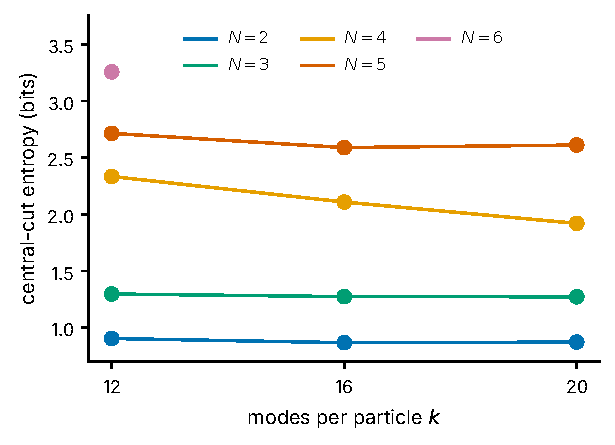
\includegraphics[width=0.6\textwidth]{figures/fig_kconv.pdf}
\caption{Central-cut entropy against the number of modes per particle (correlated start).}
\label{fig:kconv}
\end{figure}

\paragraph{Checks.} The machinery was tested on one-particle problems with known answers (Table~\ref{tab:checks}). The closed form of $\Gamma_\infty$ quoted in Section~\ref{sec:mc} was checked against the numerically summed column of the kinetic operator for $M=64,\dots,65536$ in one dimension; the fitted exponent against $M$ is $\num{p_UV}$.

\begin{table}[ht]
\centering
\footnotesize
\caption{Checks of the numerical machinery on one-particle problems with known answers.}
\label{tab:checks}
\begin{tabular}{L{6.8cm}ccc}
\toprule
Check & computed & reference & relative difference \\
\midrule
Real-time propagation, weak barrier ($A=1$): splitting & 0.791910 & 0.791776 & $\ensuremath{1.7\times10^{-4}}$ \\
Instanton formula against exact diagonalization, $A=8$ & 0.2010 & 0.1913 & 5.0\% \\
\bottomrule
\end{tabular}
\end{table}


\paragraph{Data.} Every number in the text and tables and every figure is generated from stored run logs and time series; entropies, correlation graphs and the extrapolation are derived from them without hand-entered values.

\section{The spectrum of the start: methods, table and checks}
\label{app:static}

This appendix holds everything behind Section~\ref{sec:static}: the method, one table of every case computed (Table~\ref{tab:start}), the structural checks and the remarks on what cannot be established. Nothing here is propagated in time.

\paragraph{What was computed.} For each $(N,k)$ the resonance tilt $c^\ast$ was found as for the main runs (the ground state has $\langle\Op\rangle=\frac12$), the lowest eigenlevels of $\hat H_N$ in the $k$-mode basis were computed (dense diagonalization when $k^N\le8000$, thick-restart Lanczos (ARPACK) otherwise, with $40$ levels, doubled to $80$ and $160$ until the coverage reaches $0.99$ or the memory limit), and the weight $|\langle\text{level}|\text{start}\rangle|^2$ of the correlated start on each was stored with the energy and the multiplicity ($N=5$, $k=24$ has a Lanczos list only). Runs at $k=6,8$ are not used: the six-mode basis crowds the all-left state into too few modes, and their energies are artefacts. Where the coverage stays below $0.99$ the weight $B_2$ of the pair is a lower bound, within $1-\text{coverage}$ of its value (the unresolved levels lie higher in energy). Levels closer than $10^{-6}$ are merged and their weights added.

\paragraph{The pair, and the gated pair.} The pair is the two levels of largest weight in the start, with $J=(E_b-E_a)/2$ and total weight $B_2$; the three distance classes of Table~\ref{tab:start} are measured from the nearer level of the pair. The \emph{gated pair} of Section~\ref{sec:measured} is a different object: the pair of low levels of smallest splitting $\Delta E$ that passes the doublet gates (mixed by $\hat O$, one particle apart in $\langle\hat O\rangle$). It is selected by its splitting, not by its weight, so it need not be the pair that carries the weight, and for $N\ge4$ it is not; where the two differ, the pair is the reading that measures how few-level the start is. A clean gated pair also gives the ratio $g_N=\Delta E_2/\Delta E_N$ of Eq.~\eqref{eq:Tobs}.

\begin{table}[ht]
\centering
\footnotesize
\setlength{\tabcolsep}{3.2pt}
\caption{The correlated start in the eigenbasis of $\hat H$, every case computed (method in the text of this appendix). $c^*$: resonance tilt of the mode basis; coverage: weight of the start on the computed levels. \emph{Pair}: the two levels of largest weight, their splitting $2J$ and total weight $B_2$. \emph{Outside the pair}: the weight on the other levels by distance to the nearer level of the pair (within $J$, $1$--$3J$, beyond $3J$); the remainder $1-B_2-\text{sum}$ is on levels not computed. \emph{Gated pair}: the pair of low levels of smallest splitting $\Delta E$ that passes the doublet gates, the weight of the start on it, and whether it is a clean doublet (with the ratio $g_N=\Delta E_2/\Delta E_N$ of Eq.~\eqref{eq:Tobs}, $\Delta E_2$ the grid value of Table~\ref{tab:params}); it is selected by splitting, not by weight, so it can differ from the pair. Rows marked $^\ast$ are Lanczos lists only; $k=6,8$ are omitted (artefacts of the small basis).}
\label{tab:start}
\begin{tabular}{rrcccccccccc}
\toprule
 & & & & \multicolumn{2}{c}{pair} & \multicolumn{3}{c}{outside the pair} & \multicolumn{3}{c}{gated pair} \\ \cmidrule(lr){5-6}\cmidrule(lr){7-9}\cmidrule(lr){10-12}
$N$ & $k$ & $c^*$ & coverage & $2J$ & $B_2$ & $<J$ & $1$--$3J$ & $\ge3J$ & $\Delta E$ & weight & clean / $g_N$ \\
\midrule
2 & 12 & 0.70 & 1.000 & 0.180 & 0.976 & 0.000 & 0.014 & 0.010 & 0.180 & 0.98 & yes / 1.06 \\
2 & 16 & 0.70 & 1.000 & 0.185 & 0.976 & 0.000 & 0.011 & 0.012 & 0.185 & 0.98 & yes / 1.03 \\
2 & 20 & 0.70 & 1.000 & 0.192 & 0.978 & 0.000 & 0.010 & 0.013 & 0.192 & 0.98 & yes / 0.99 \\
\addlinespace[2pt]
3 & 12 & 1.46 & 1.000 & 0.189 & 0.938 & 0.000 & 0.044 & 0.017 & 0.189 & 0.94 & yes / 1.01 \\
3 & 16 & 1.36 & 1.000 & 0.191 & 0.952 & 0.000 & 0.018 & 0.030 & 0.191 & 0.95 & yes / 1.00 \\
3 & 20 & 1.31 & 1.000 & 0.193 & 0.955 & 0.000 & 0.017 & 0.028 & 0.193 & 0.96 & yes / 0.98 \\
\addlinespace[2pt]
4 & 12 & 2.26 & 0.993 & 0.184 & 0.668 & 0.085 & 0.213 & 0.027 & 0.052 & 0.46 & no \\
4 & 16 & 2.14 & 0.985 & 0.225 & 0.845 & 0.001 & 0.114 & 0.026 & 0.104 & 0.34 & no \\
4 & 20 & 2.02 & 0.986 & 0.218 & 0.906 & 0.000 & 0.056 & 0.024 & 0.218 & 0.91 & yes / 0.87 \\
4 & 24 & 1.94 & 0.975 & 0.220 & 0.921 & 0.000 & 0.042 & 0.012 & -- & -- & -- \\
4 & 28 & 1.87 & 0.977 & 0.220 & 0.931 & 0.000 & 0.018 & 0.028 & -- & -- & -- \\
4 & 32 & 1.82 & 0.976 & 0.221 & 0.934 & 0.000 & 0.018 & 0.024 & -- & -- & -- \\
\addlinespace[2pt]
5 & 12 & 2.92 & 0.971 & 0.362 & 0.683 & 0.268 & 0.016 & 0.004 & 0.152 & 0.35 & no \\
5 & 16 & 2.72 & 0.942 & 0.229 & 0.780 & 0.002 & 0.151 & 0.010 & 0.107 & 0.39 & no \\
5 & 20 & 2.62 & 0.943 & 0.233 & 0.812 & 0.007 & 0.114 & 0.010 & 0.105 & 0.39 & no \\
5 & 24$^\ast$ & 2.57 & 0.918 & 0.251 & 0.836 & 0.005 & 0.077 & 0.000 & -- & -- & -- \\
\addlinespace[2pt]
6 & 12 & 3.66 & 0.936 & 0.437 & 0.729 & 0.194 & 0.013 & 0.000 & 0.173 & 0.31 & no \\
\bottomrule
\end{tabular}
\end{table}


\paragraph{Reading the table.} At $N=2,3$ the two readings coincide and the pair carries almost everything. At $N=4$ the weight of the pair converges with the basis; the small-basis rows are a basis artefact, and the gated pair passes its gates only at one basis size. At $N=5$ neither the weight nor the coverage is converged, and the $k=12$ rows are dominated by levels within $J$ of the pair that vanish at larger $k$; at $N=6$ only one unconverged basis exists. The weight outside the pair that grows with $N$ is the $1$--$3J$ column; the far column is small and does not grow. Where a clean doublet exists, $g_N$ lies close to one, which supports carrying $g_N=1$ in the quantum price.

\paragraph{Reflection symmetry, sector exclusion, label fragmentation.} The reflection $R$ ($y_i\to-y_i$ for all particles) is built in the mode basis as $\prod_iP^\top R_{\rm grid}P$; the one-body parity closure of the truncated modes is about $0.05$, so eigenstate parities are near, not exactly, $\pm1$, and the small odd weights in Fig.~\ref{fig:parity} are leakage of the basis. The start is even to within this leakage ($\langle R\rangle>0.999$ at $N=3,4$). Every level of non-negligible weight is even; the levels between the two members of the pair carry no weight and are odd, so they are not a hidden manifold of transfer states. The right-valley occupation $\langle n_i\rangle$ of particle $i$ is the expectation of the one-particle valley indicator (Table~\ref{tab:levels}): the pair is carried mainly by particle $0$. The first even level with two particles on the right (sector exclusion) is far from the pair at $N=3$ and absent from the computed levels at $N=4$ (Fig.~\ref{fig:parity}). The first levels in which particle $1$ or $2$ has moved (label fragmentation) lie a few $J$ from the pair, the nearest about two $J$ away, and at $N=4$ the states of particles $1$ and $2$ already hybridize; the start has at most one to two per cent of its weight on them.

\begin{figure}[t]
\centering
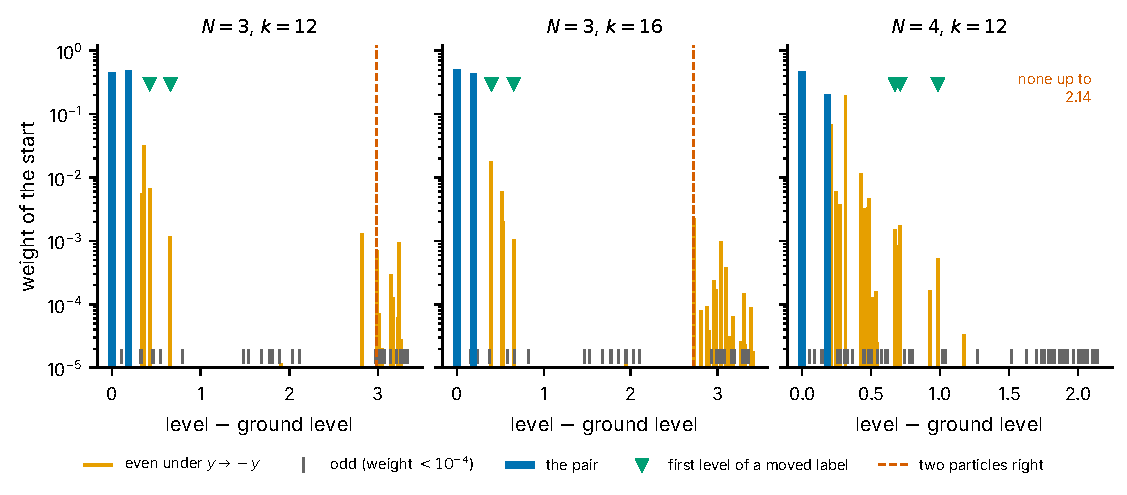
\includegraphics[width=\textwidth]{figures/fig_parity.pdf}
\caption{\textbf{Levels, their reflection parity and the weight of the start.} Lowest levels of $\hat H$ at the resonance tilt, $N=3$ ($k=12,16$) and $N=4$ ($k=12$). Orange: levels even under the reflection $y_i\to-y_i$ of all particles, with the weight of the start on them; grey ticks: odd levels (all carry less than $\num{fu_oddmax_N4_k12}$ of the start). Blue: the pair. Green triangles: the first even level in which particle $1$ (and $2$, $3$) has moved to the right valley instead of particle $0$; at $N=3$ these lie between $\num{fu_marg_lo}$ and $\num{fu_marg_hi}$ times $J$ from the pair. Red dashed: the first even level with two particles on the right; at $N=4$, $k=12$ there is none among the lowest levels computed.}
\label{fig:parity}
\end{figure}

\begin{table}[ht]
\centering
\footnotesize
\caption{The lowest levels of $\hat H$ that carry weight of the start ($N=3$, $k=16$, resonance tilt): energy above the ground state, weight of the start, reflection parity $\langle R\rangle$ and right-valley occupation $\langle n_i\rangle$ of each particle. The pair (levels 0 and 2) is carried mainly by particle $0$; level 1 is odd under the reflection and carries no weight; levels 5 and 9 are the first in which particle $1$, then particle $2$, has moved.}
\label{tab:levels}
\begin{tabular}{rccccccc}
\toprule
level & $E-E_0$ & weight & $\langle R\rangle$ & $\langle n_0\rangle$ & $\langle n_1\rangle$ & $\langle n_2\rangle$ \\
\midrule
0 & 0.000 & 0.5102 & +1.000 & 0.52 & 0.04 & 0.02 \\
1 & 0.157 & 0.0000 & -1.000 & 0.47 & 0.02 & 0.01 \\
2 & 0.191 & 0.4415 & +1.000 & 0.45 & 0.15 & 0.03 \\
5 & 0.396 & 0.0178 & +1.000 & 0.02 & 0.74 & 0.04 \\
9 & 0.652 & 0.0011 & +1.000 & 0.01 & 0.01 & 0.88 \\
\bottomrule
\end{tabular}
\end{table}


\paragraph{The cosine counts} of Fig.~\ref{fig:cosines} come from a greedy pursuit with joint refit of the amplitudes, with the frequency of each new cosine scanned on the residual, applied to the stored signal $\langle\Op\rangle(t)$, $0\le t\le200$; at most eight cosines are tried. They are free fits, not predictions.

\paragraph{Tabulating the observable.} The observable is a function of positions, so $|f'(t)|\le N\|K_x\|$ with $\|K_x\|=\pi^2/(2\Delta x^2)=\num{fu_Kx}$ on the grid of this paper, and $f$ can be tabulated to the allowed error $\varepsilon\|\Op\|$ on about $\num{fu_tab_points}$ points for every $N$. This is the reason no reduction-based hardness statement is possible for the fixed family (Section~\ref{sec:regimeend}).

\paragraph{Reproduction.} Every number and figure of this section is computed from the stored level lists, level files and signal fits by the scripts of the repository; the companion report lists which file feeds which object.

\section{The quantum cost model}
\label{app:quantum}

Each particle's grid state takes $n_p=\num{n_p}$ qubits, and the register adds $\num{b_aux}$ qubits of arithmetic workspace and control. A qubitization step is one query to a selection oracle that costs $C_{\rm sel}=2C_{\rm QFT}+C_W(b)$ T-gates, the cost of two Fourier transforms plus one evaluation of the pair potential at fixed-point precision $b=\num{b_fix}$ bits; the latter dominates, and the total is
$C_{\rm sel}=\num{C_sel}$. The Hamiltonian is written as a linear combination of unitaries with one-norm $\lambda=N\lambda_U+\binom N2\lambda_W$, with $\lambda_U=\num{lam_U}$ (the trap maximum on the grid) and $\lambda_W=V_{\rm cap}=\num{lam_W}$, so that the T-gate count is
\begin{equation}
T_{\rm qub}=\big\lceil\lambda\,\Tobs+\ln(1/\varepsilon)\big\rceil\,C_{\rm sel},\qquad \Tobs=\Tobs(N,\mut)\ \text{of Eq.~\eqref{eq:Tobs} with } g_N=1.
\end{equation}
The product-formula count is a second-order step count $r=\lceil\Tobs\sqrt{\Lambda/\varepsilon}\rceil$ with the commutator sum $\Lambda(N)=N\lambda_1+\binom N2\lambda_2$, $\lambda_2=2\max|\nabla W|^2/m=\num{lam_two}$, times the cost per step. One step applies, for each particle, the kinetic factor (two Fourier transforms and a phase, $2C_{\rm QFT}+n_p$ T-gates) and the trap factor ($n_p$), and, for each pair, the pair potential once per Gaussian in the fit of the capped pair wall, so the cost per step is $N(2C_{\rm QFT}+2n_p)+\binom N2K\,C_W$ with $K=\num{k_gauss}$ Gaussians. Because both counts are linear in $\Tobs$, their ratio does not depend on the mass; its size is set by $\lambda_2$,
the squared slope of the capped pair wall, and it is why the product formula falls out of the window at small $N$.

\paragraph{What the model omits.}
Two terms are omitted at leading order and restored in the ``complete'' edge of Table~\ref{tab:quantum}: the mass dependence of the trap frequency in the semiclassical prefactor of Eq.~\eqref{eq:Tobs} ($\omega\propto m^{-1/2}$ along the mass axis of a fixed trap), and the kinetic one-norm $\lambda_{\rm kin}=\num{lam_kin}/m_{\rm rel}$. Restoring both lowers the edge by $\num{edge_shift_8}$ at $N=8$.
Not modelled: preparation of the correlated start, error-correction overheads beyond the T-gate count, repeated measurements for precision $\varepsilon$ on a bounded observable. The semiclassical form of Eq.~\eqref{eq:Tobs} is an interpolation anchored at the measured
switching time at $\mut_0=\num{mut0}$, not an ab-initio law (Section~\ref{sec:model}).


\bibliographystyle{unsrt}
\bibliography{main}

\end{document}
